\section{Evaluation Tasks}
\label{sec:tasks}

This appendix contains the tasks given to users during the evaluations in Chapter~\ref{chap:eval}

\subsection{First Task}
\label{sec:task1}

This was the task for the first evaluation that took place in October 2013.  Details can be found in Section~\ref{sec:eval1}.  The two levels of preparation of the task are below.

\begin{enumerate}
\item Start a new `visualisation' session.
\item Call it what you like.
\item Open the file r\_asrc\_20\_fake\_whole\_cell.csv
\item Allocate the species to their appropriate cell locations
\item Annotate the graph
\item Save it
\item Play the animation
\item Attach the saved picture of the graph to the session
\end{enumerate}

Open up a graph of the r\_arc\_20\_fake\_whole\_cell.csv experiment.  Annotate and save the graph.  Run the experiment visually.  Attach the previously saved graph to the session.

\subsection{Second Task}
\label{sec:task2}

This was the task for the second and third evaluations that took place in February and March 2014 respectively.  Details can be found in Sections~\ref{sec:eval2}~and~\ref{sec:eval3}.  The two levels of preparation of the task are below.

\begin{enumerate}
\item Start a new `visualisation' session.
\item Give it a title
\item Open the file r\_asrc\_20\_fake\_whole\_cell.csv
\item Select the model file december\_2012\_locations.csv
\item Annotate the graph
\item Annotate the animation
\item Save it
\item Close the program
\item Reopen the program
\item Load the previously saved file
\item Change the colour of one of the lines
\item Undo your changes
\item Normalise the graphs
\item Export the data
\item Play the animation
\end{enumerate}

Start a new session, add some annotations to the graph and the cells, save your changes.  Restart the program and load your previous session.  Change the plots appearance and then undo your changes.  Then normalise and export your data.  Finally play the animation

\clearpage

\section{Questionnaires and Results}
\label{sec:qs}

\begin{figure}[h!]
    \centering
    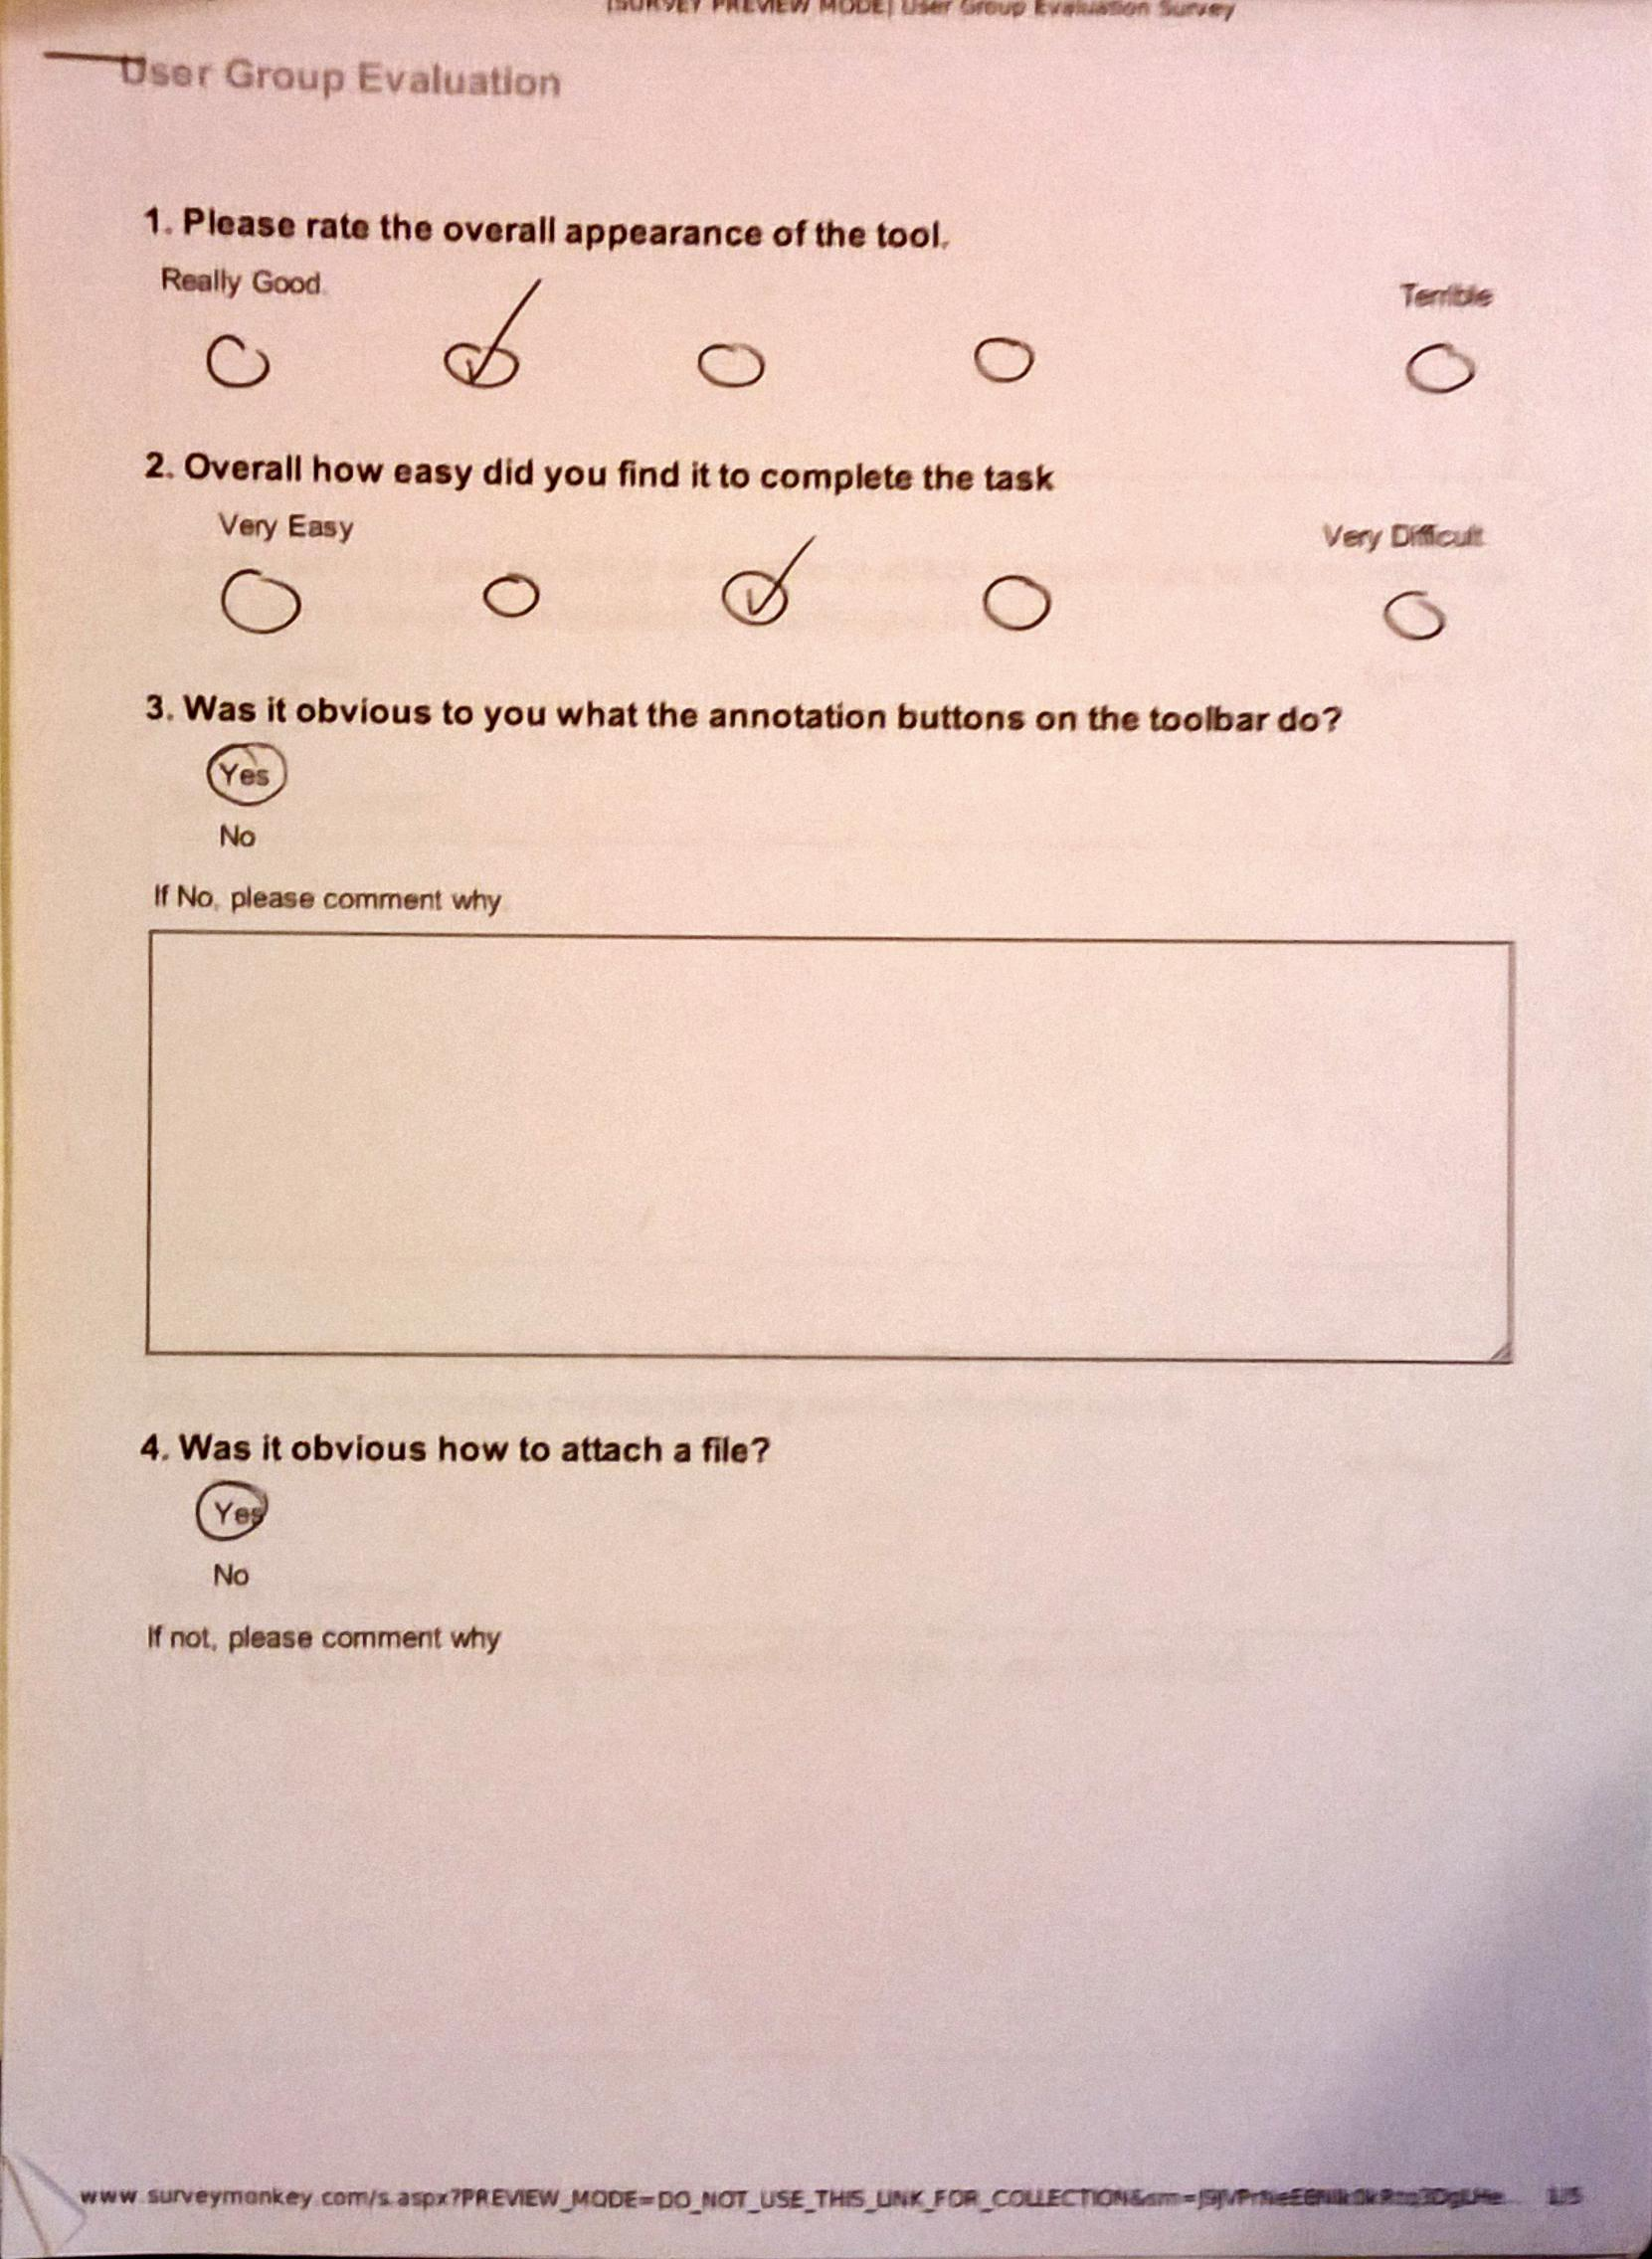
\includegraphics[width=0.95\textwidth]{images/user_eval/user_eval_1.jpg}
    \caption{First Evaluation}
\end{figure}

\begin{figure}[h!]
    \centering
    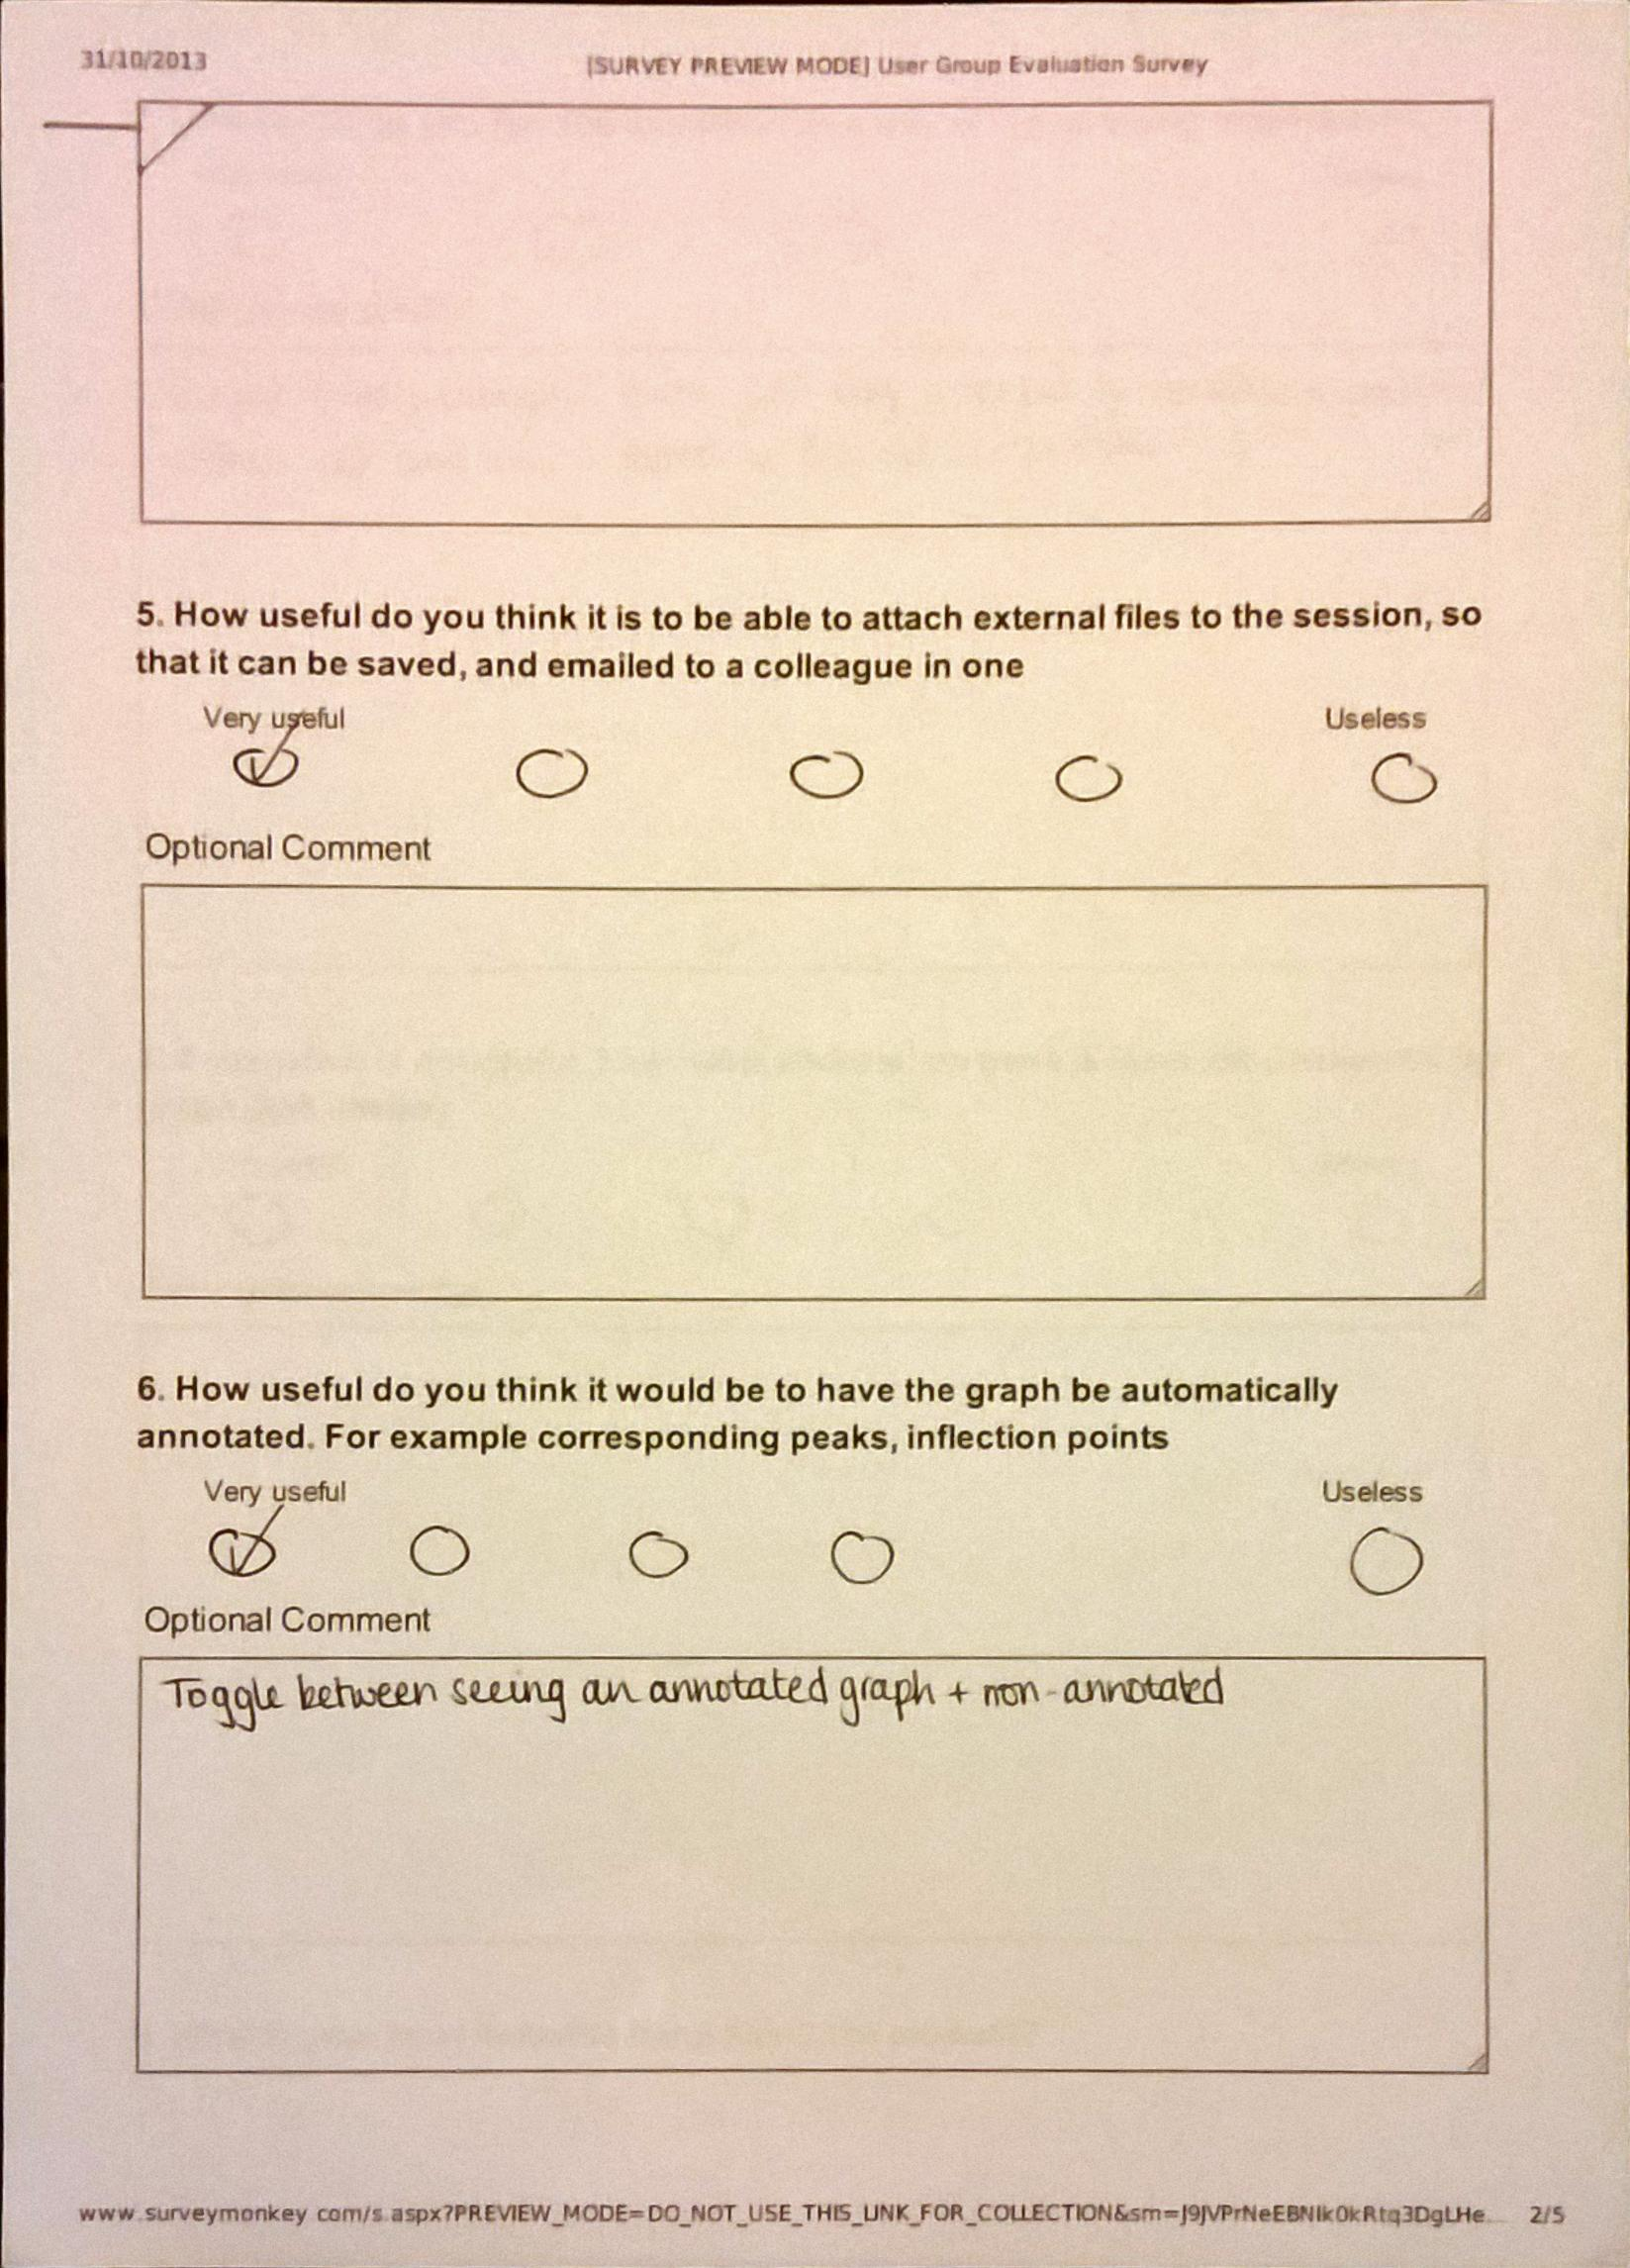
\includegraphics[width=0.95\textwidth]{images/user_eval/user_eval_2.jpg}
    \caption{First Evaluation}
\end{figure}

\begin{figure}[h!]
    \centering
    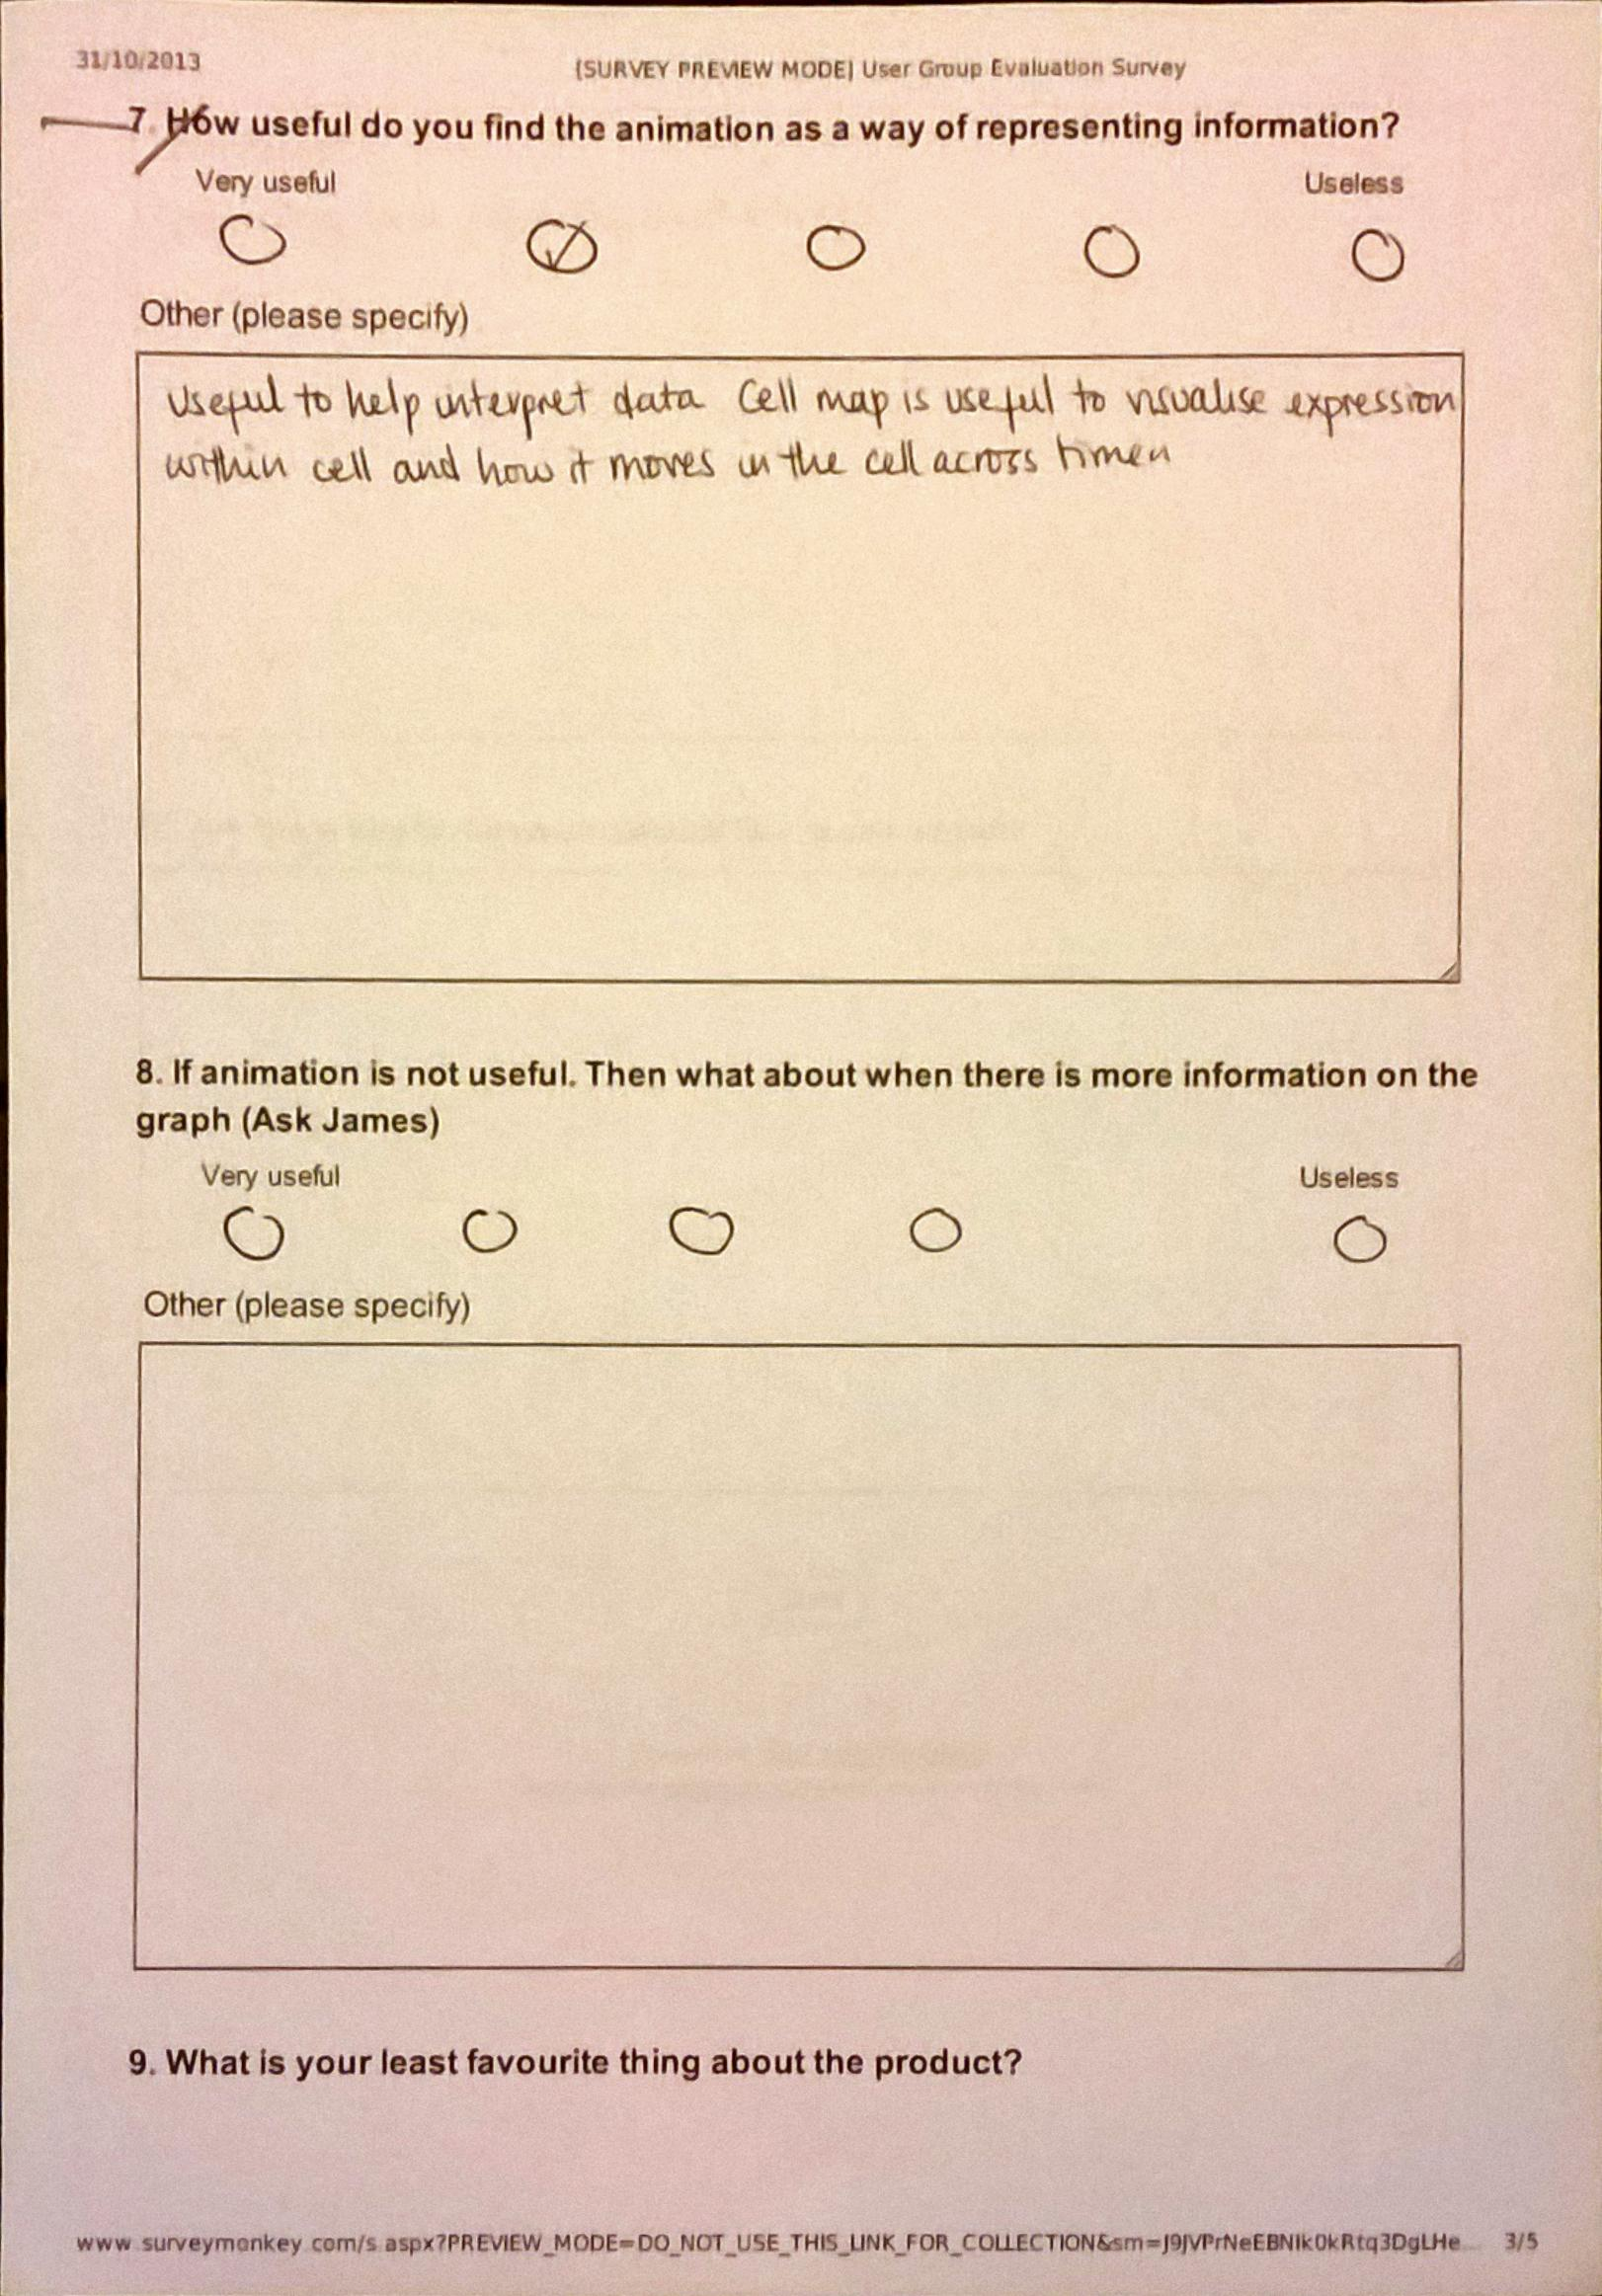
\includegraphics[width=0.95\textwidth]{images/user_eval/user_eval_3.jpg}
    \caption{First Evaluation}
\end{figure}

\begin{figure}[h!]
    \centering
    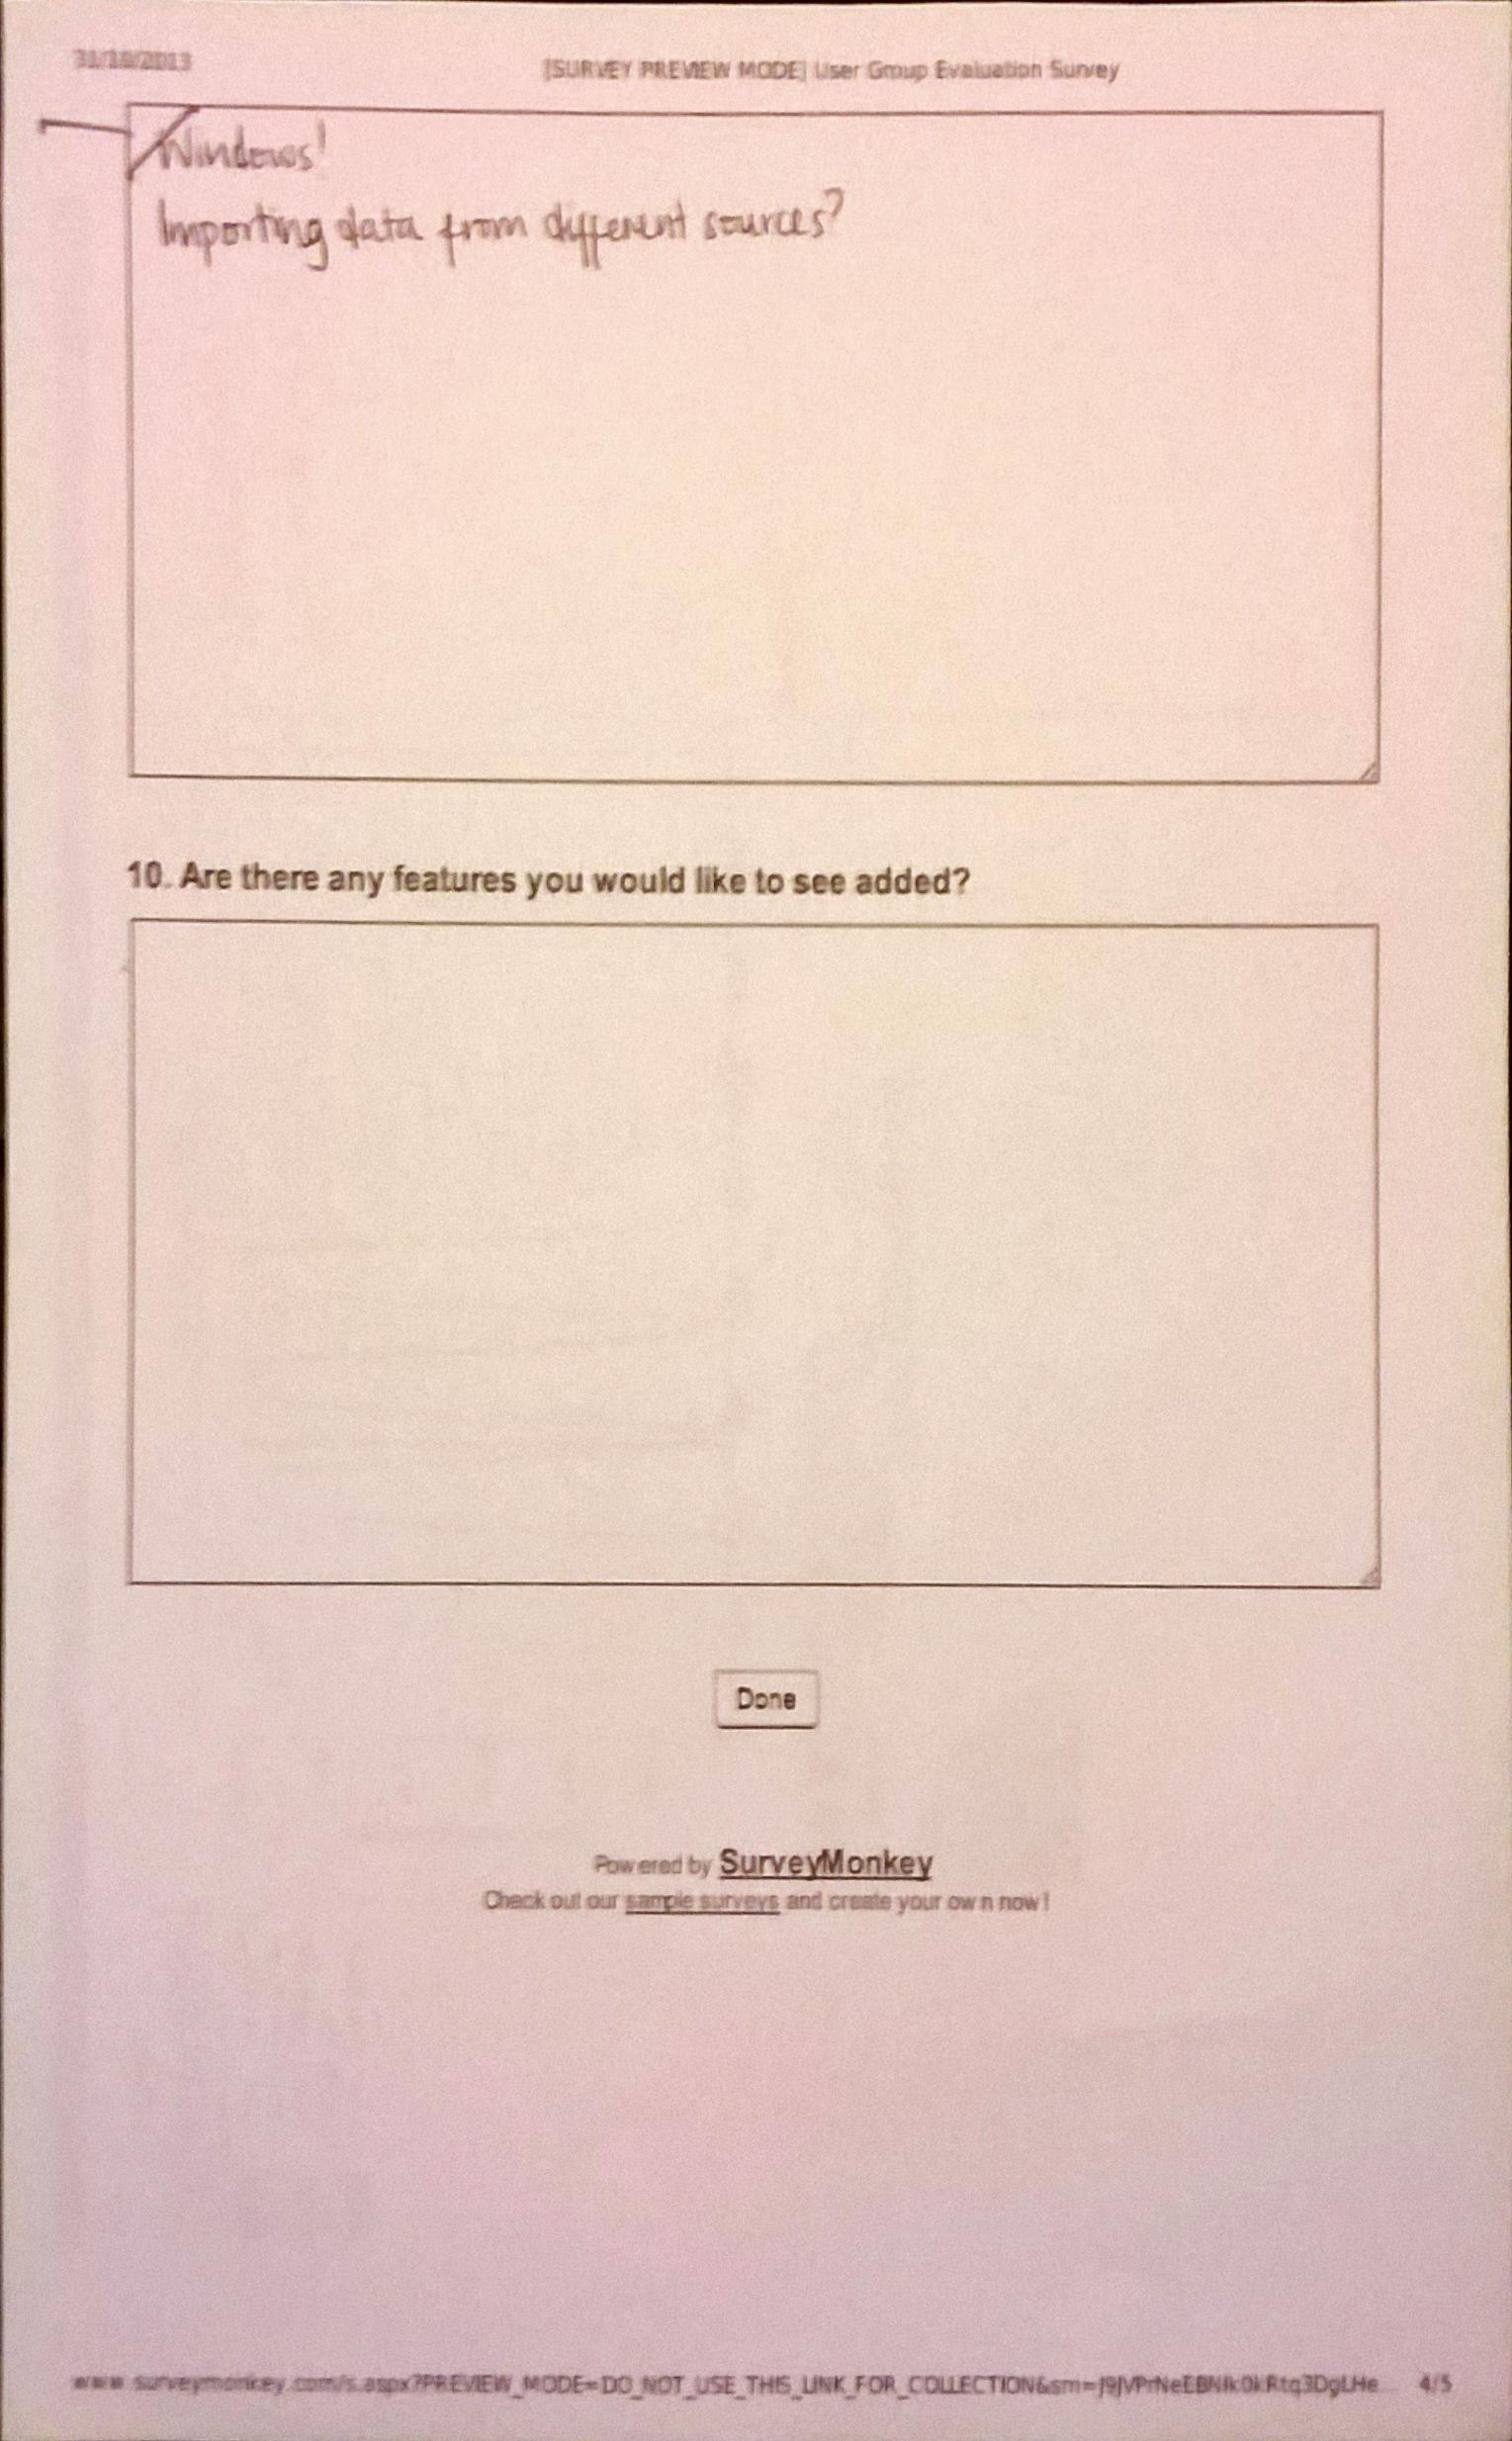
\includegraphics[width=0.95\textwidth]{images/user_eval/user_eval_4.jpg}
    \caption{First Evaluation}
\end{figure}

\begin{figure}[h!]
    \centering
    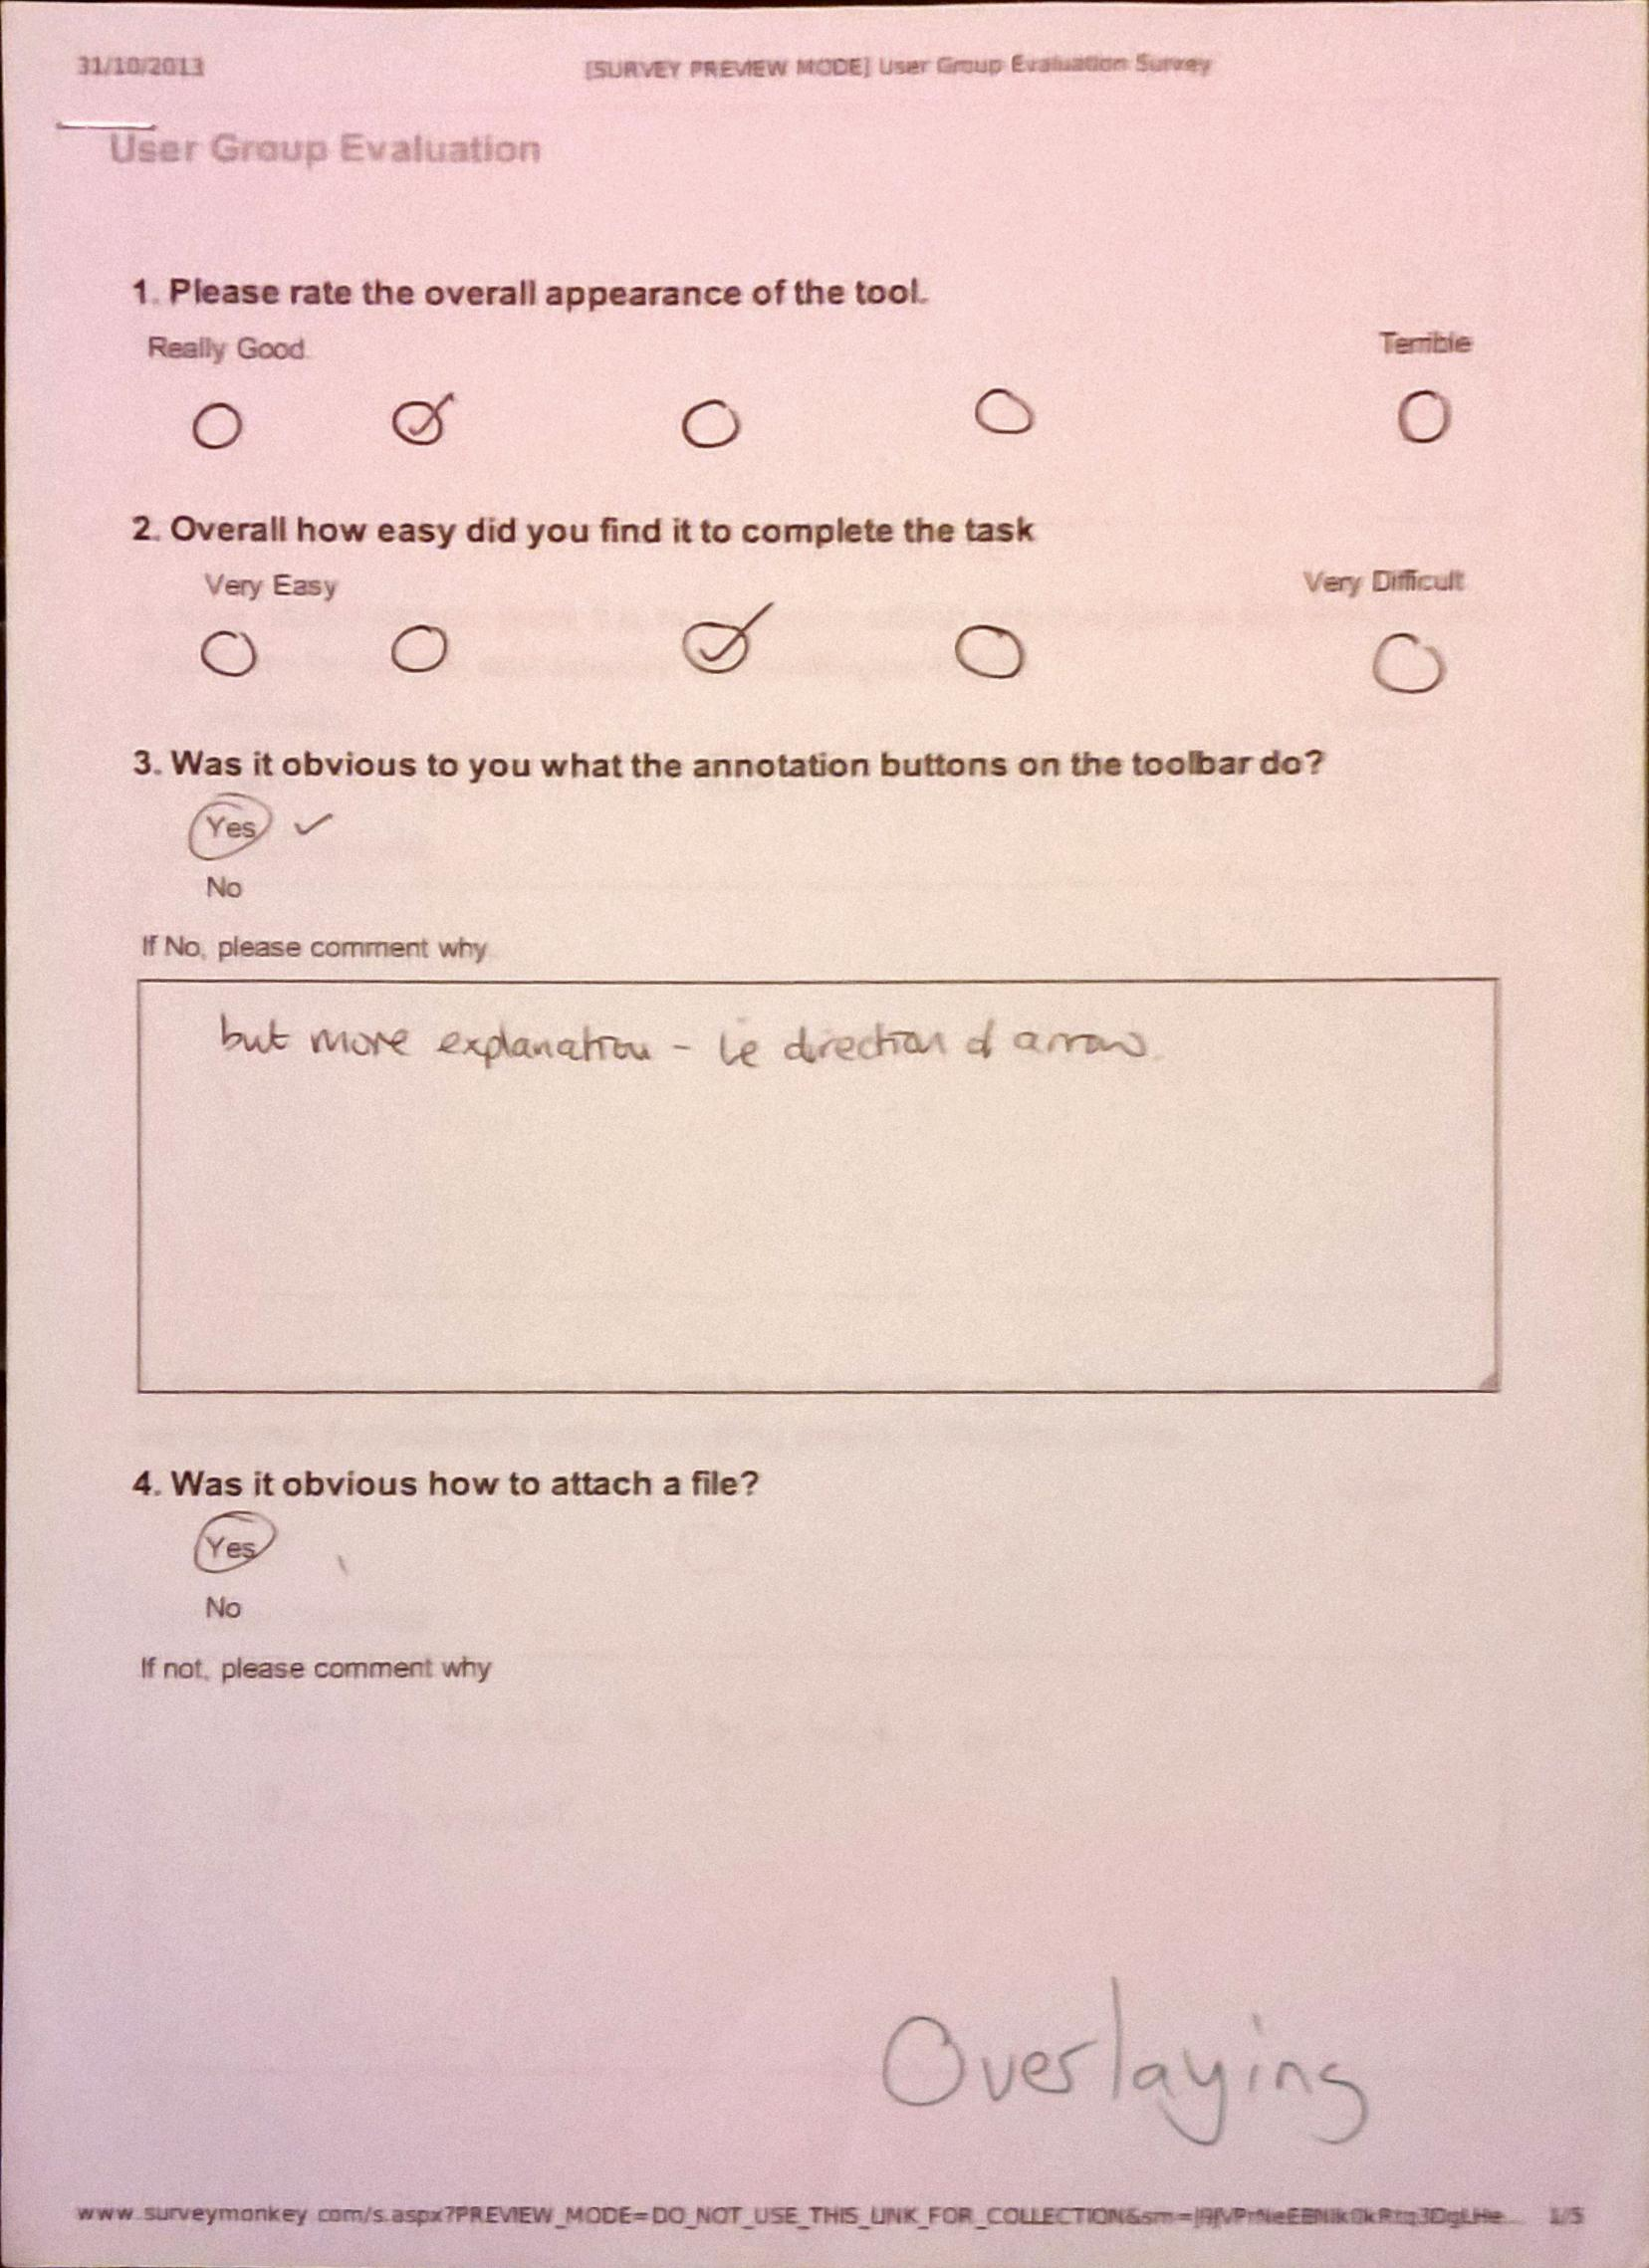
\includegraphics[width=0.95\textwidth]{images/user_eval/user_eval_5.jpg}
    \caption{First Evaluation}
\end{figure}

\begin{figure}[h!]
    \centering
    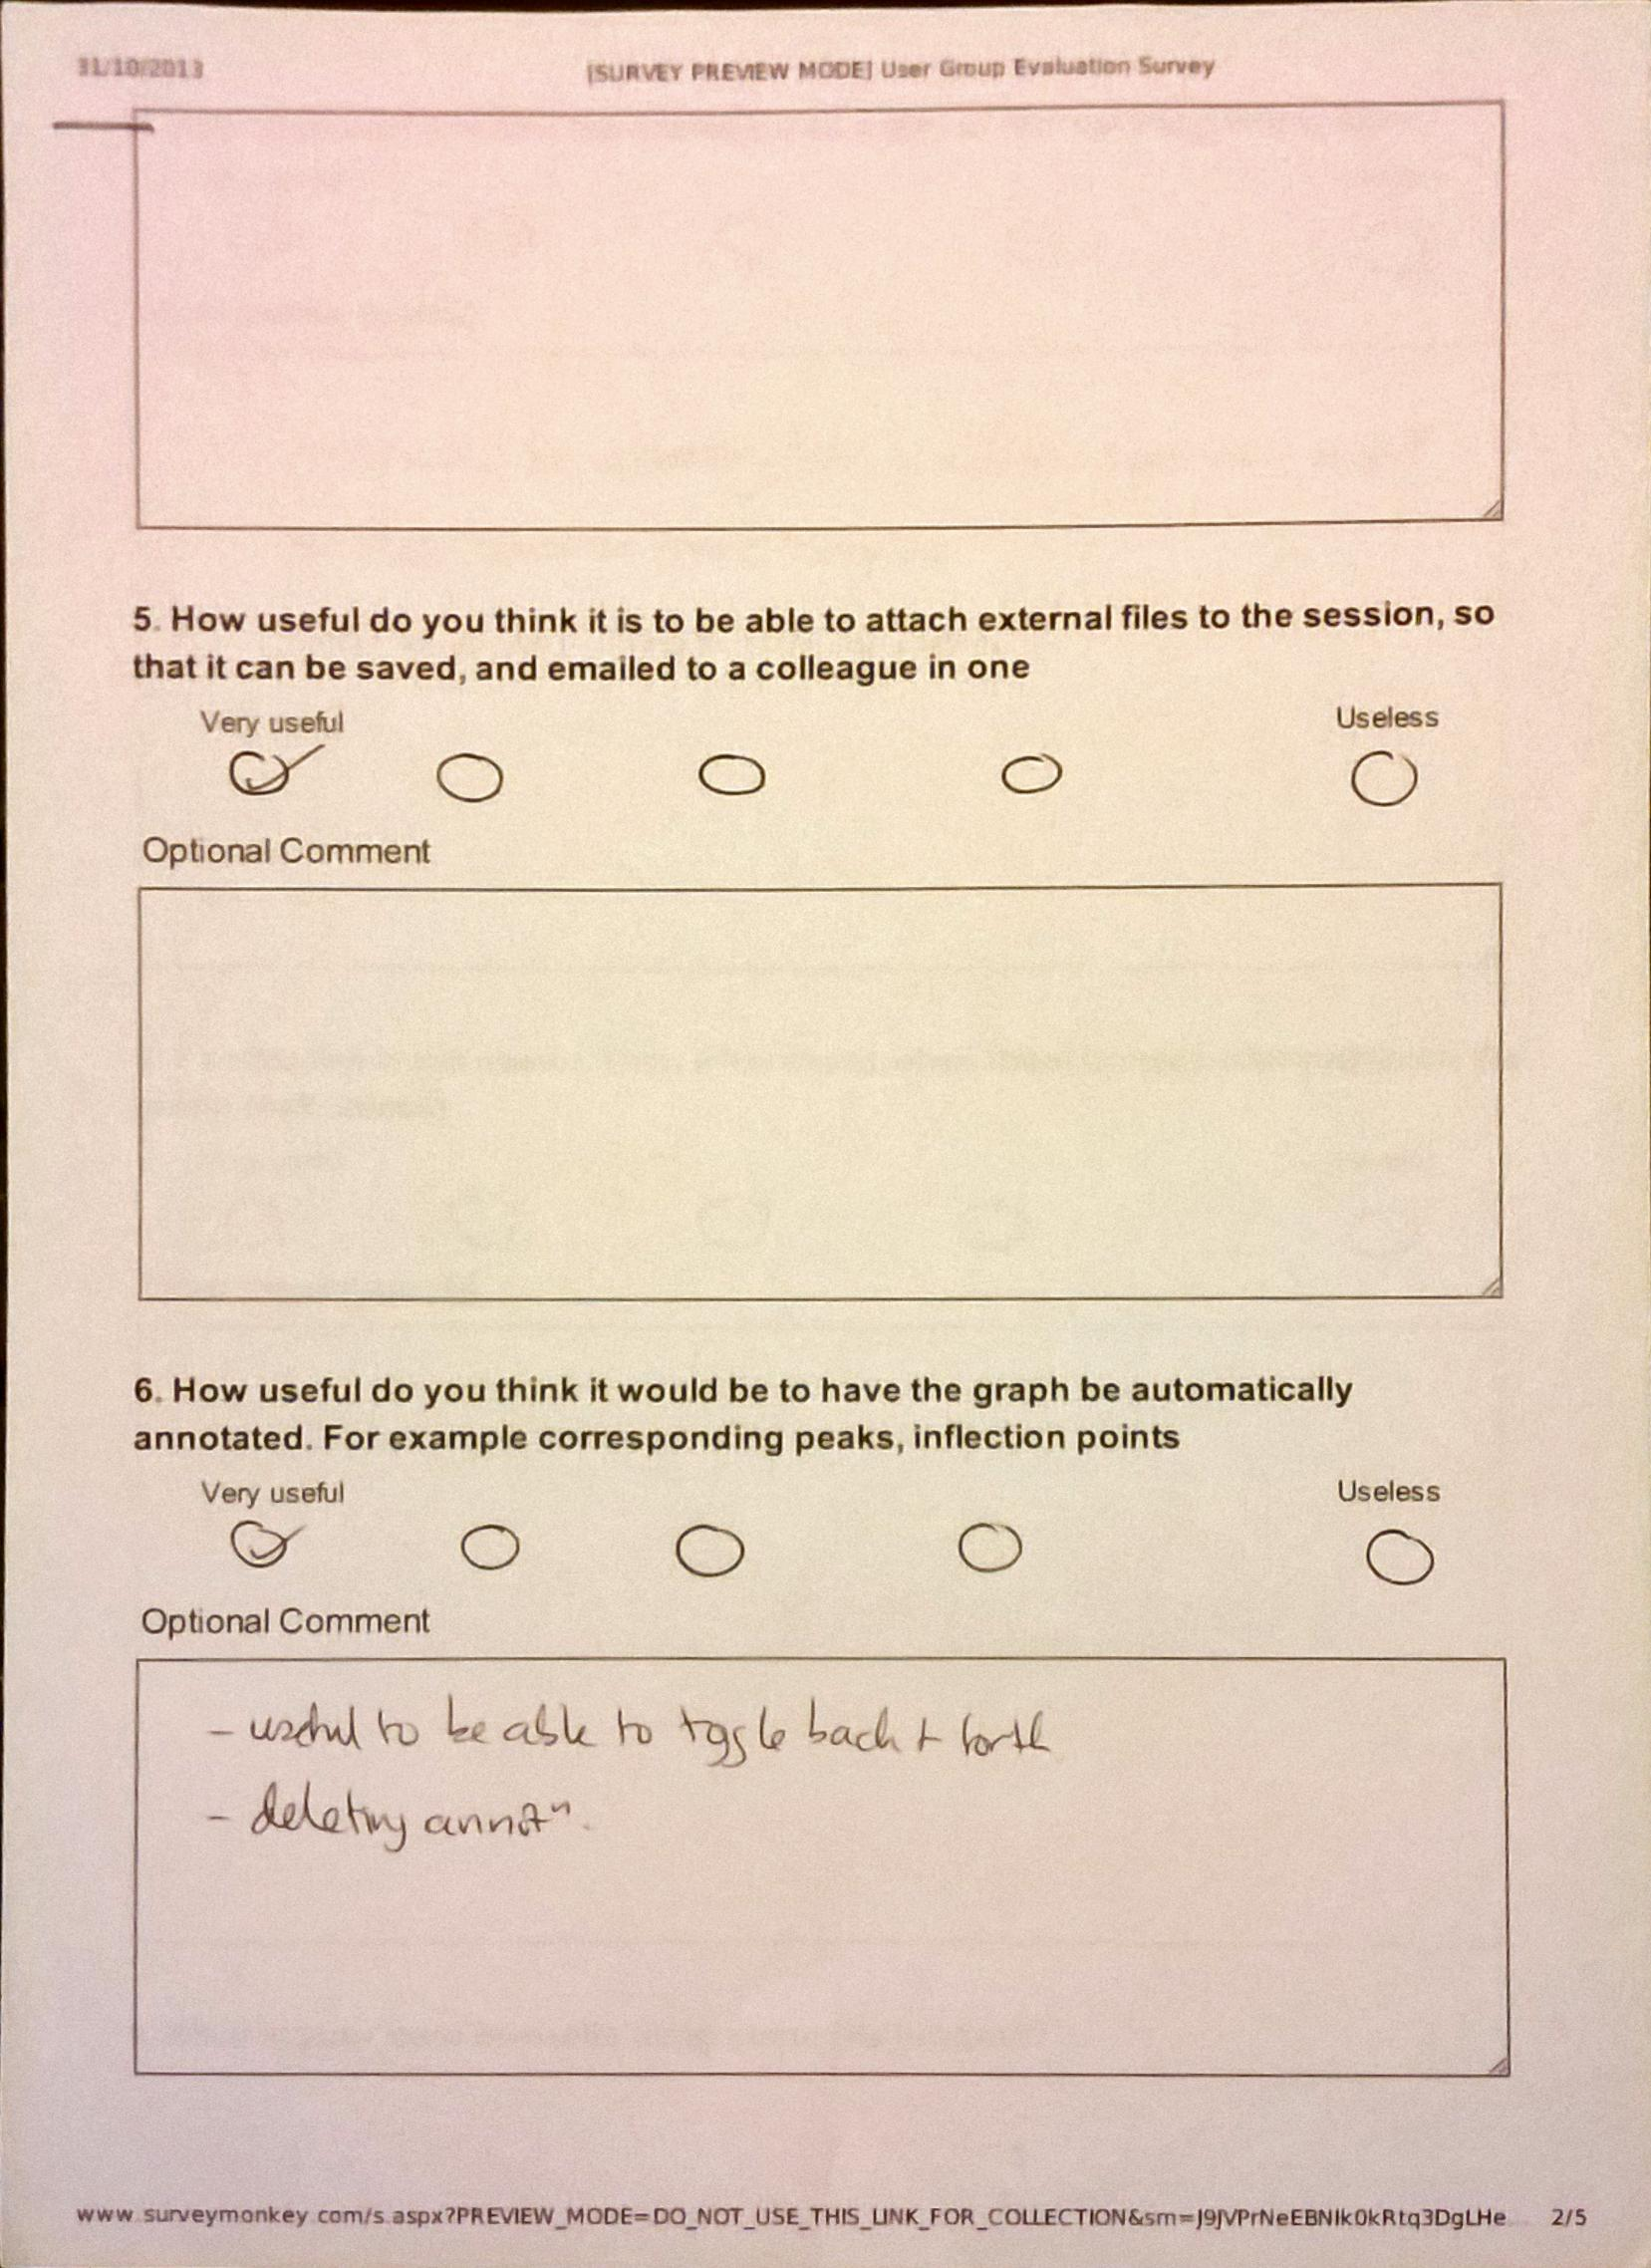
\includegraphics[width=0.95\textwidth]{images/user_eval/user_eval_6.jpg}
    \caption{First Evaluation}
\end{figure}

\begin{figure}[h!]
    \centering
    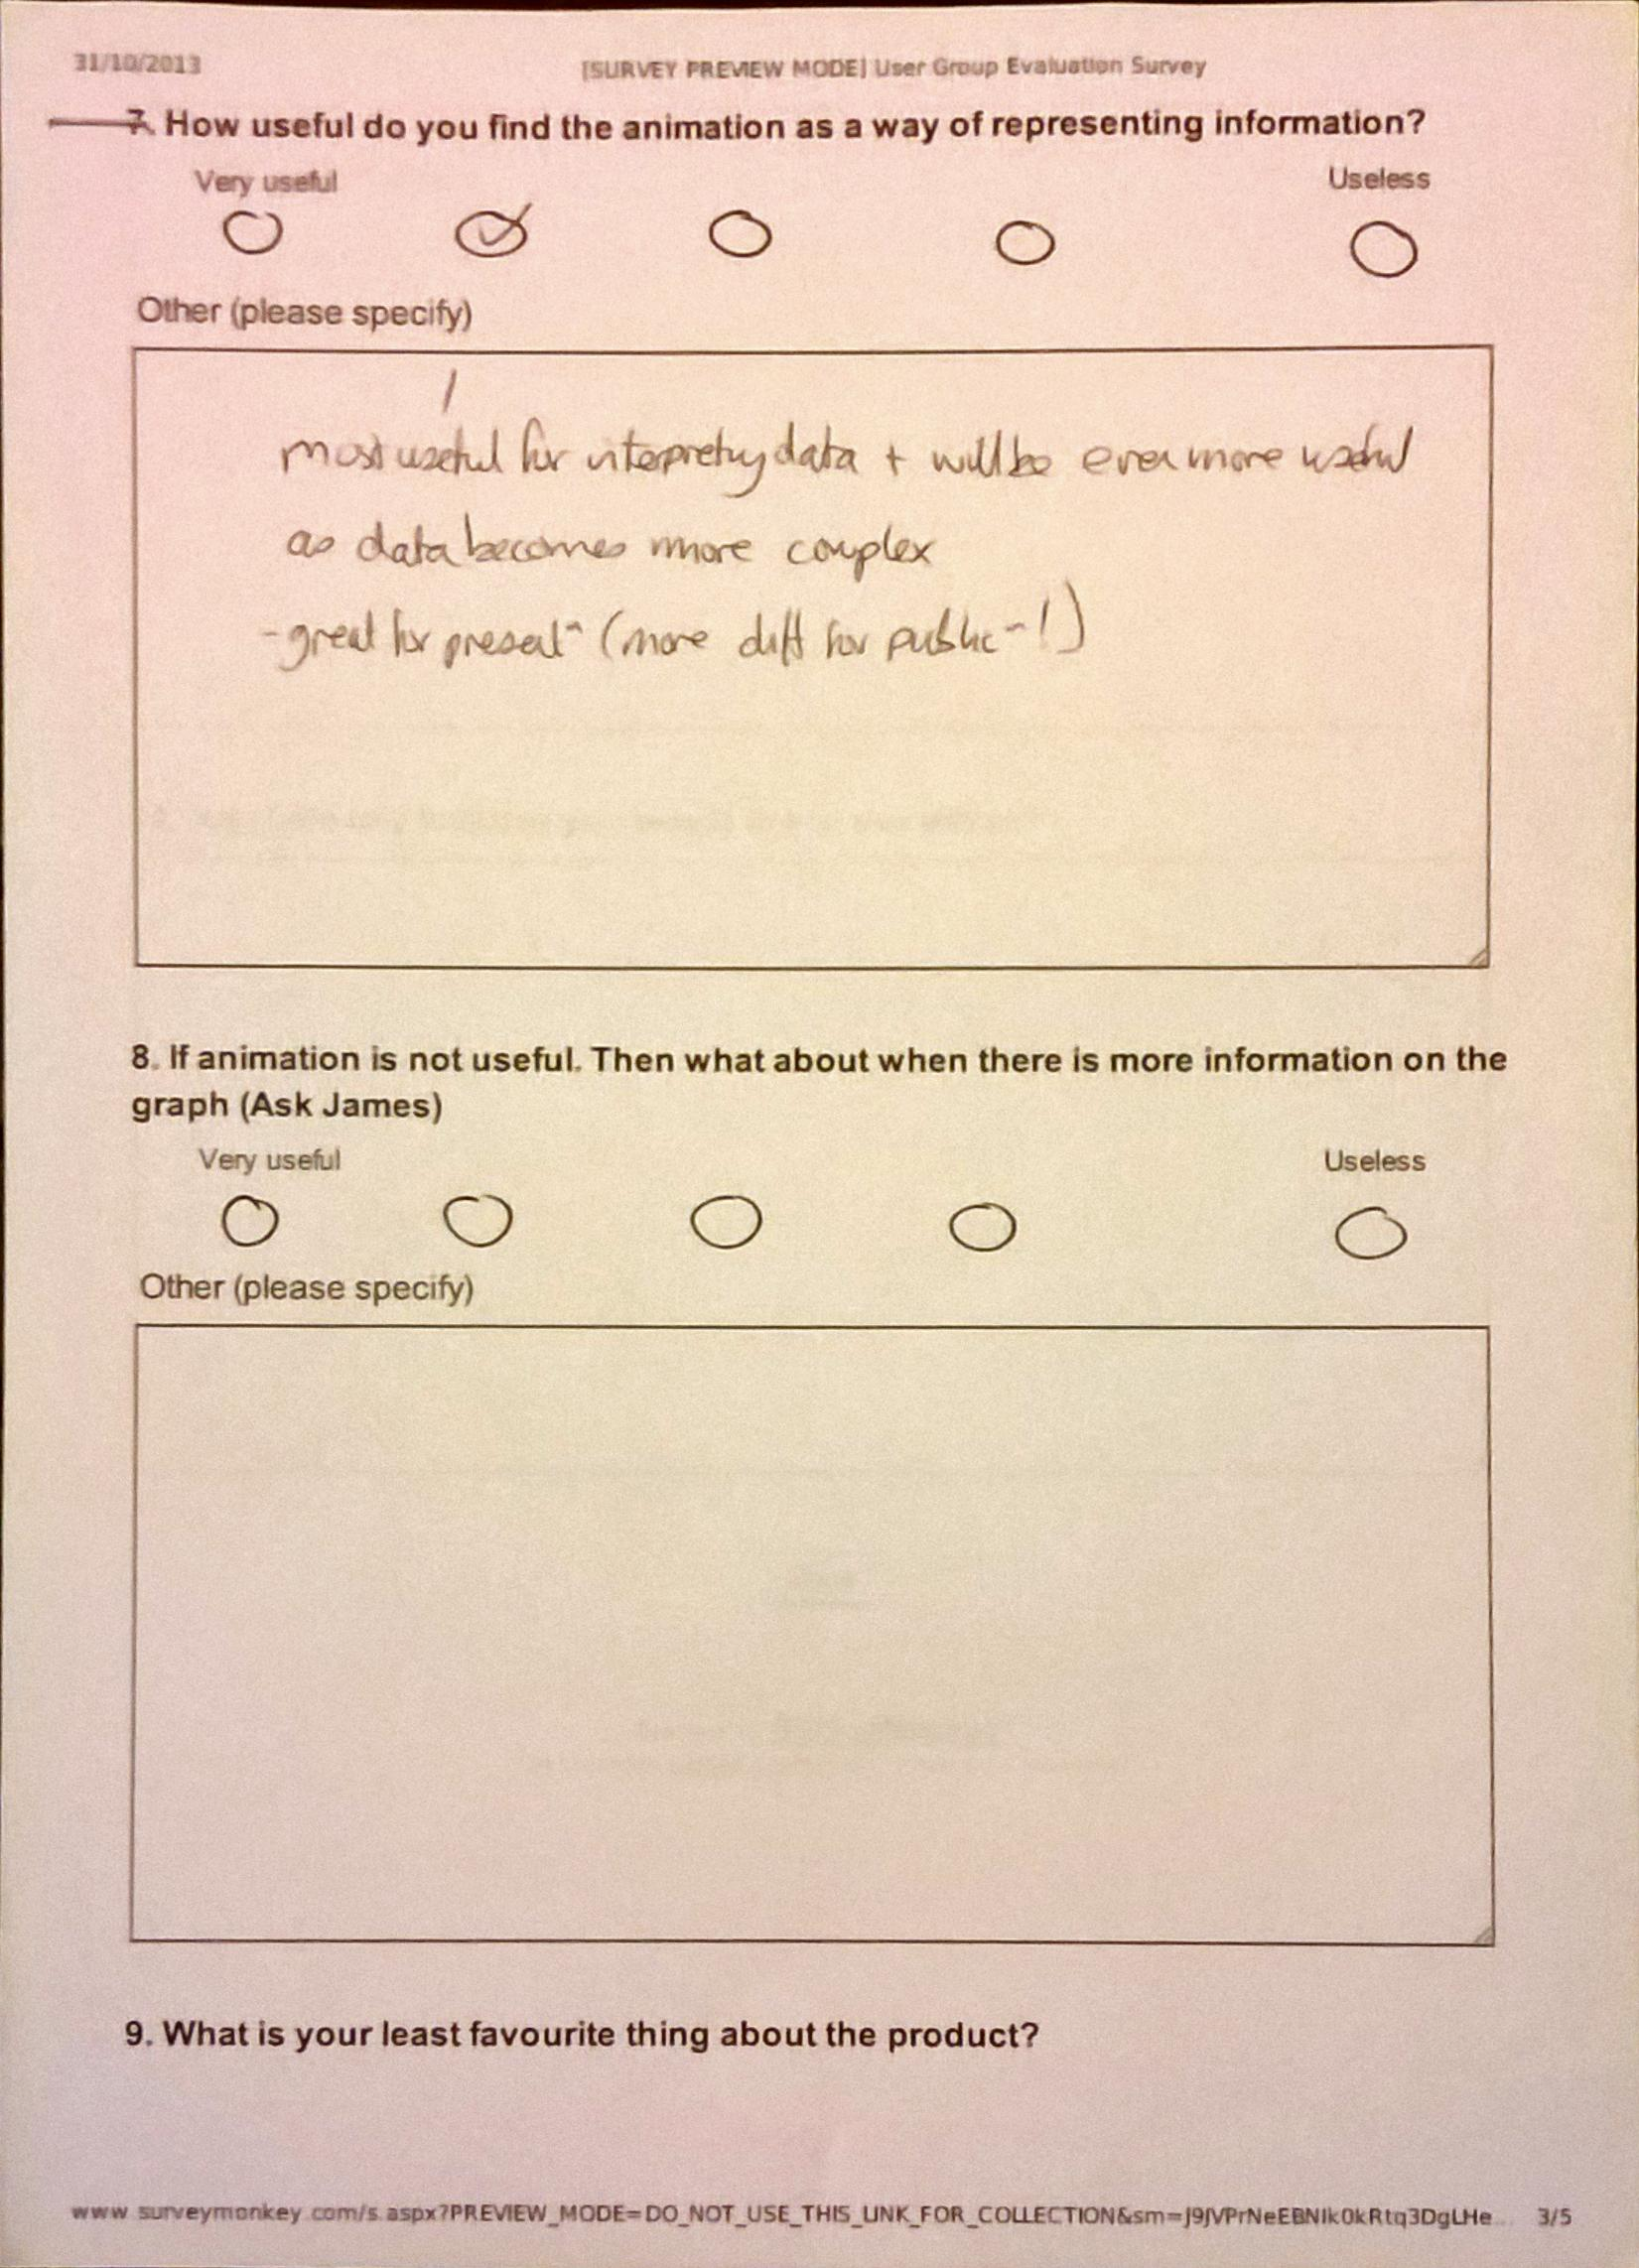
\includegraphics[width=0.95\textwidth]{images/user_eval/user_eval_7.jpg}
    \caption{First Evaluation}
\end{figure}

\begin{figure}[h!]
    \centering
    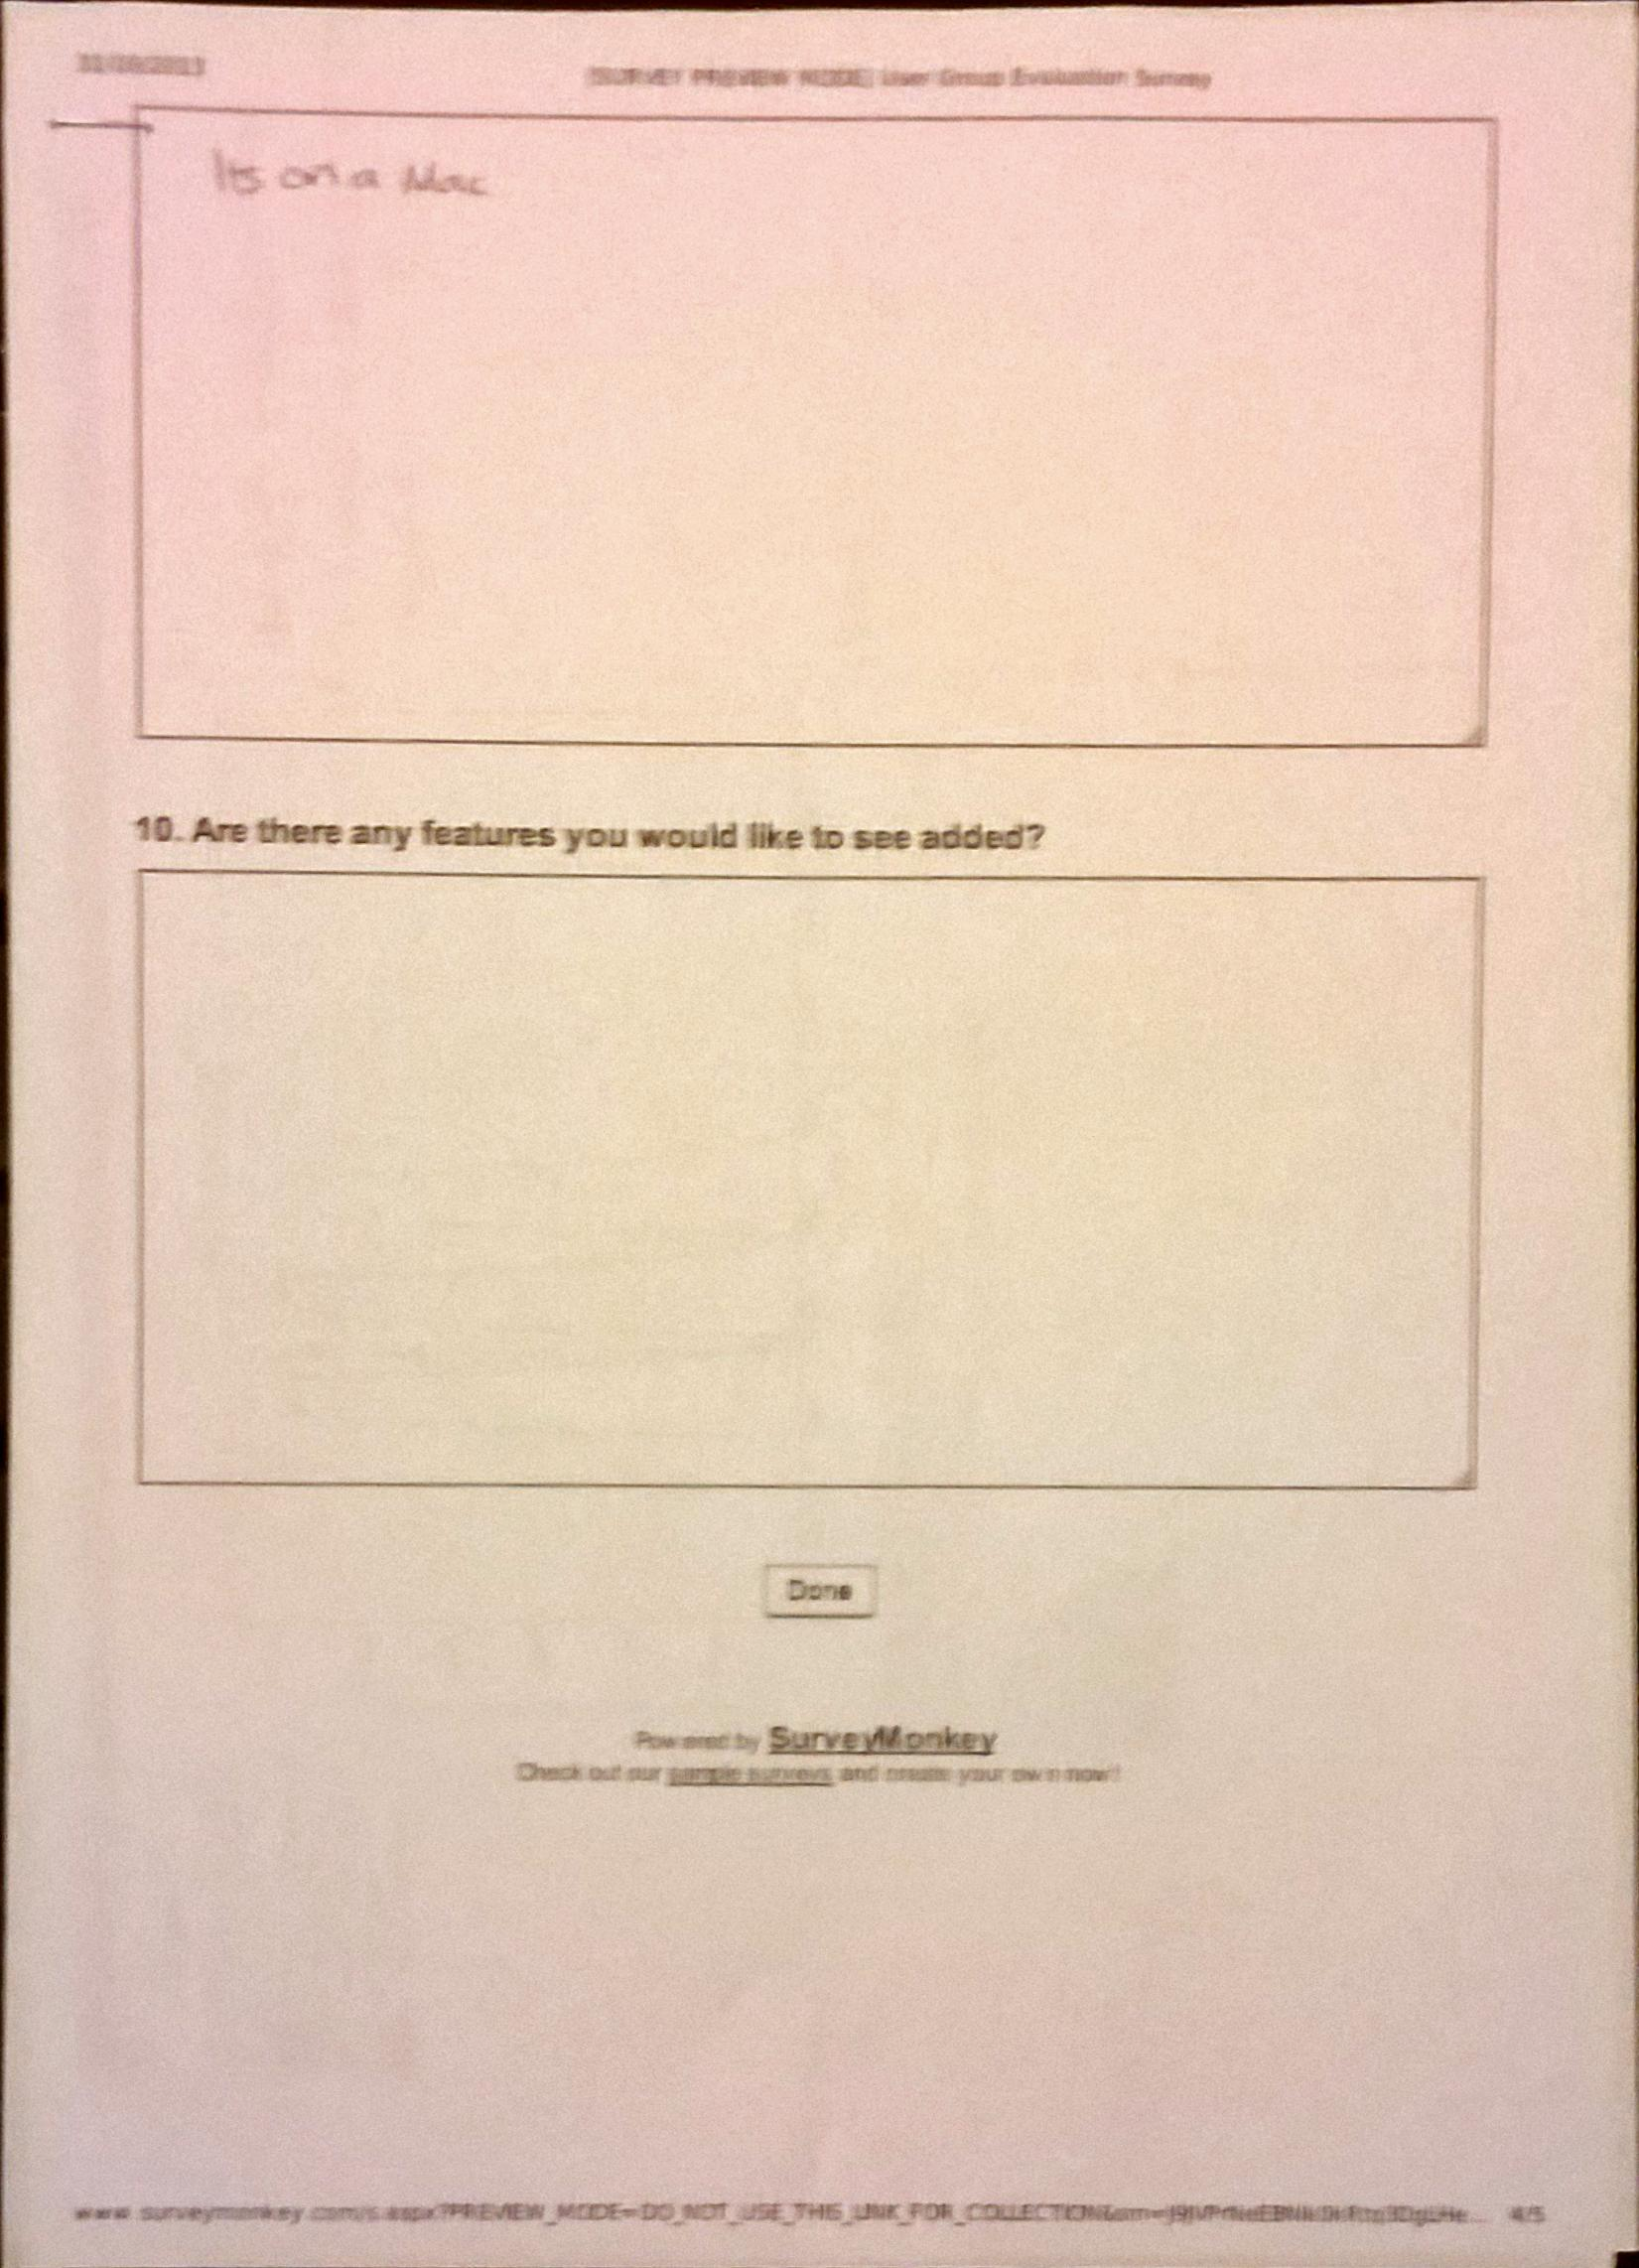
\includegraphics[width=0.95\textwidth]{images/user_eval/user_eval_8.jpg}
    \caption{First Evaluation}
\end{figure}

\begin{figure}[h!]
    \centering
    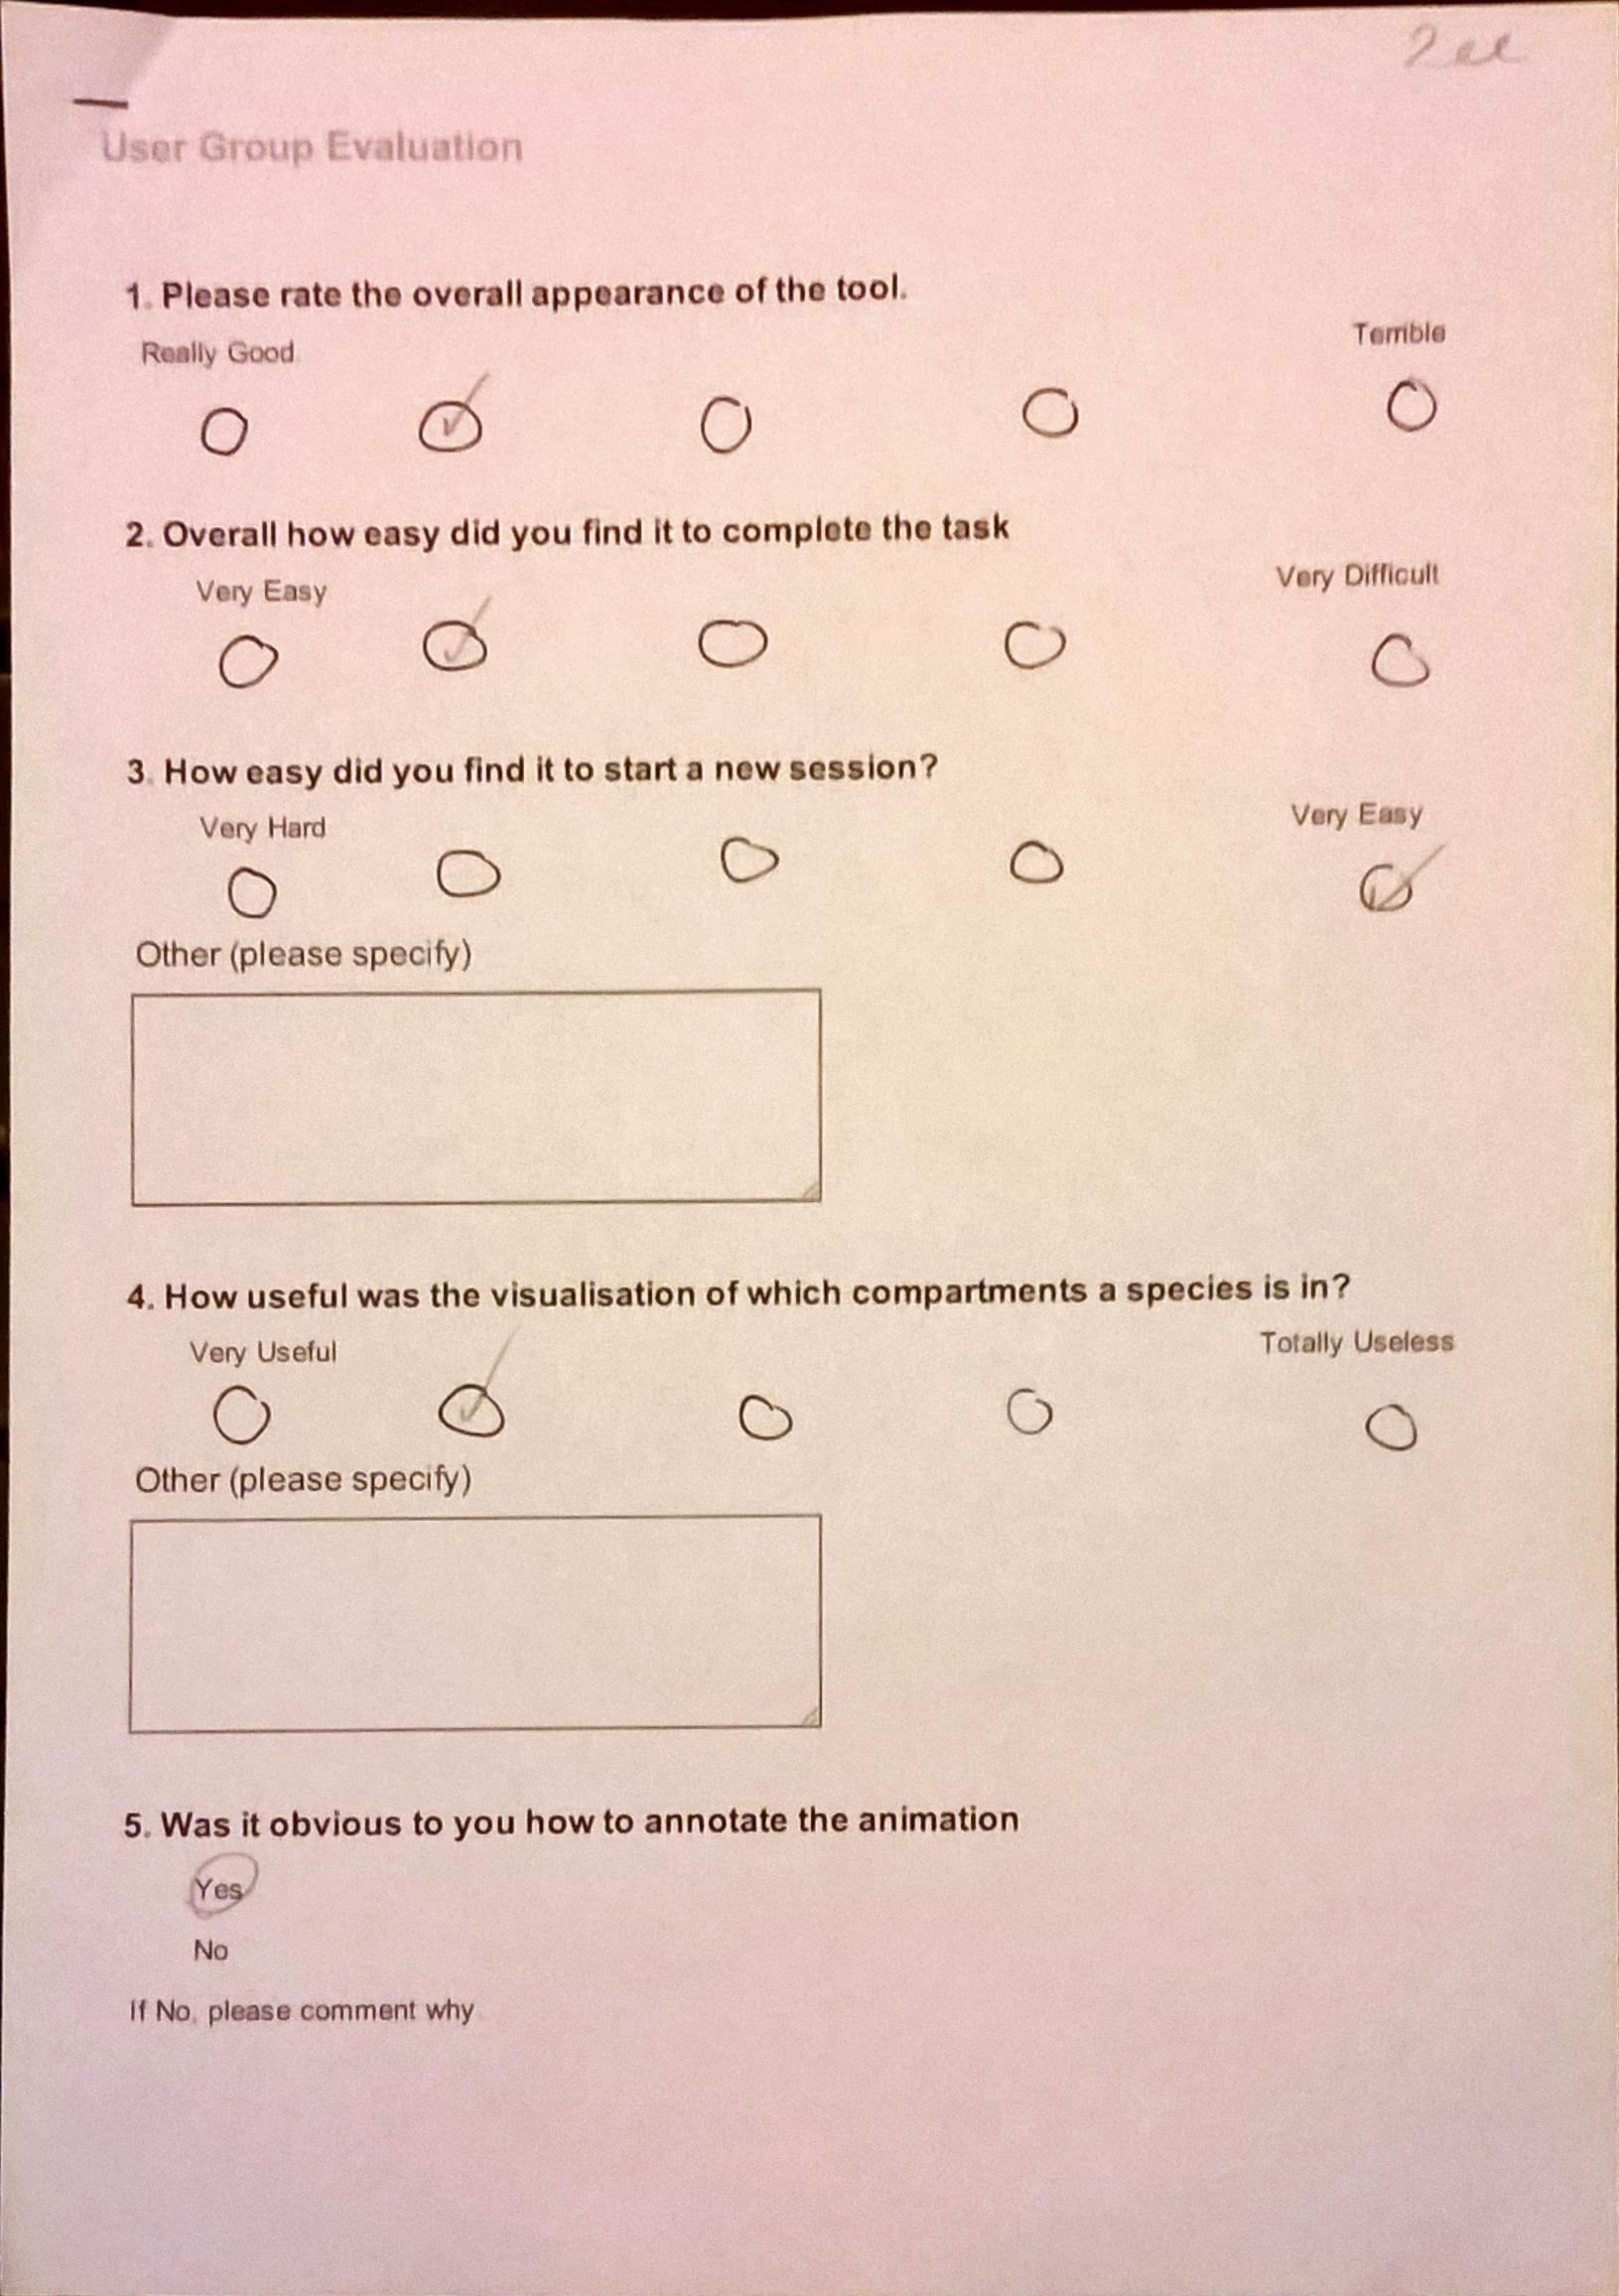
\includegraphics[width=0.95\textwidth]{images/user_eval/user_eval_9.jpg}
    \caption{Second Evaluation}
\end{figure}

\begin{figure}[h!]
    \centering
    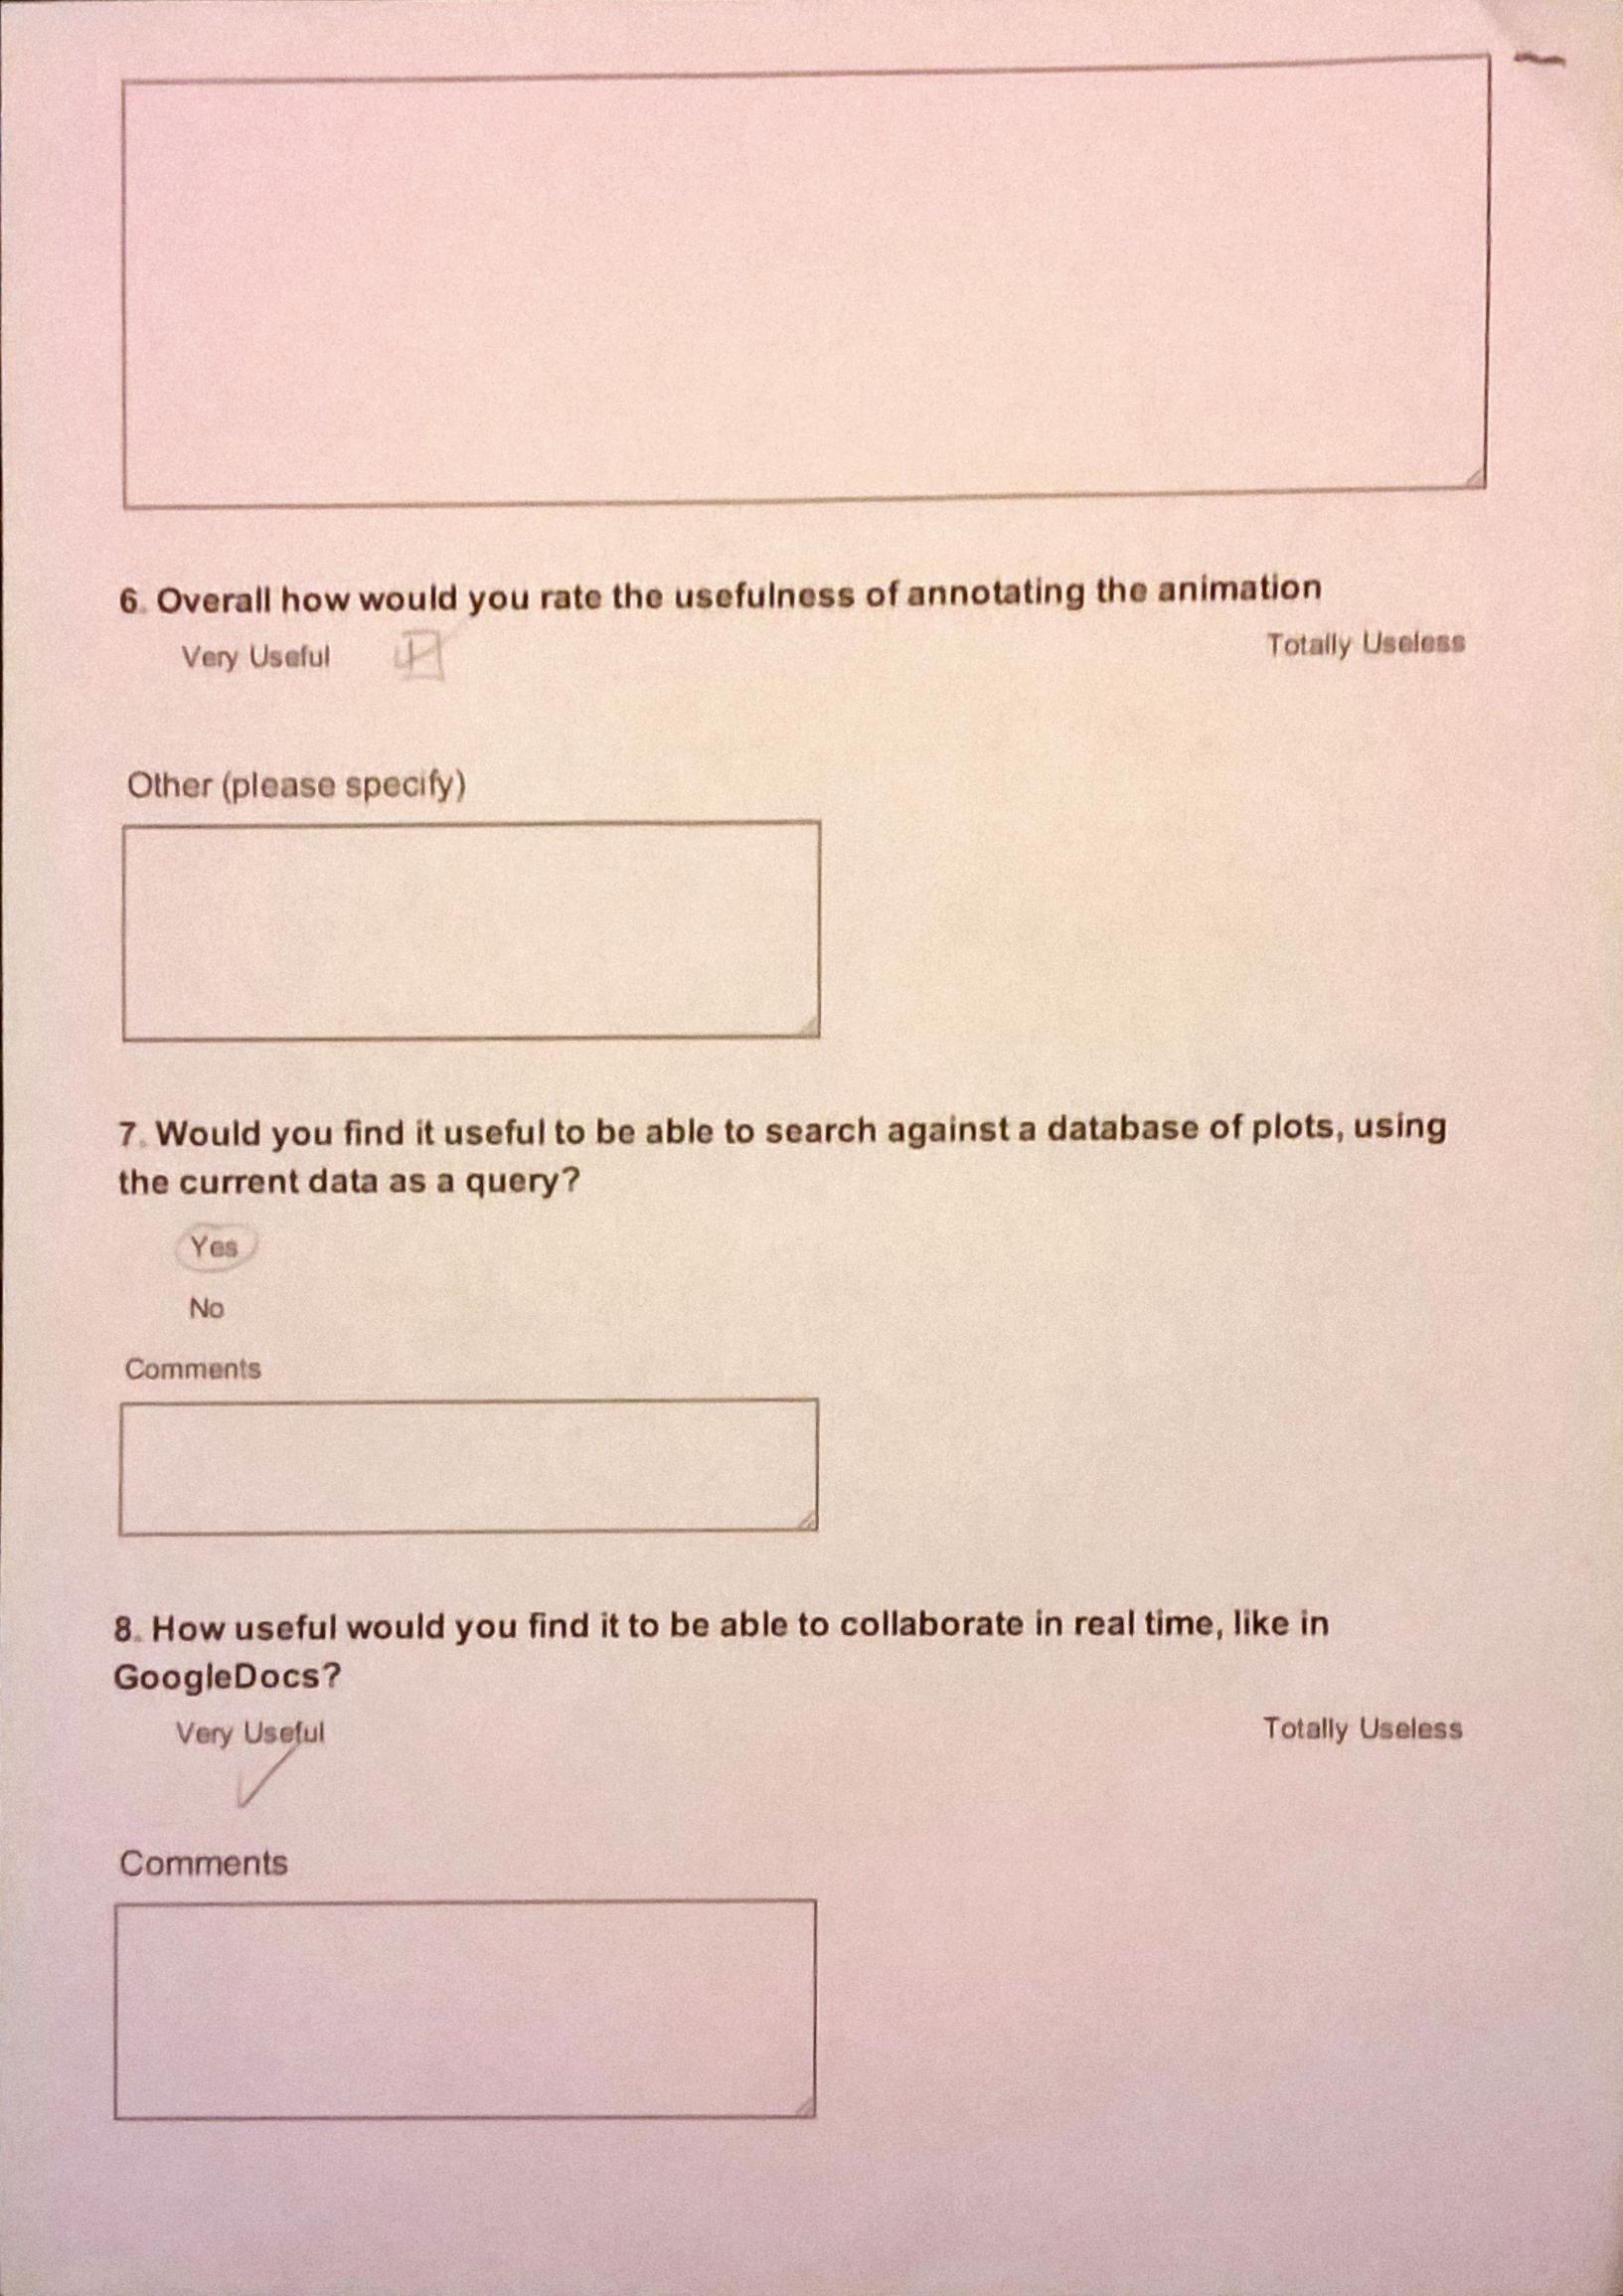
\includegraphics[width=0.95\textwidth]{images/user_eval/user_eval_10.jpg}
    \caption{Second Evaluation}
\end{figure}

\begin{figure}[h!]
    \centering
    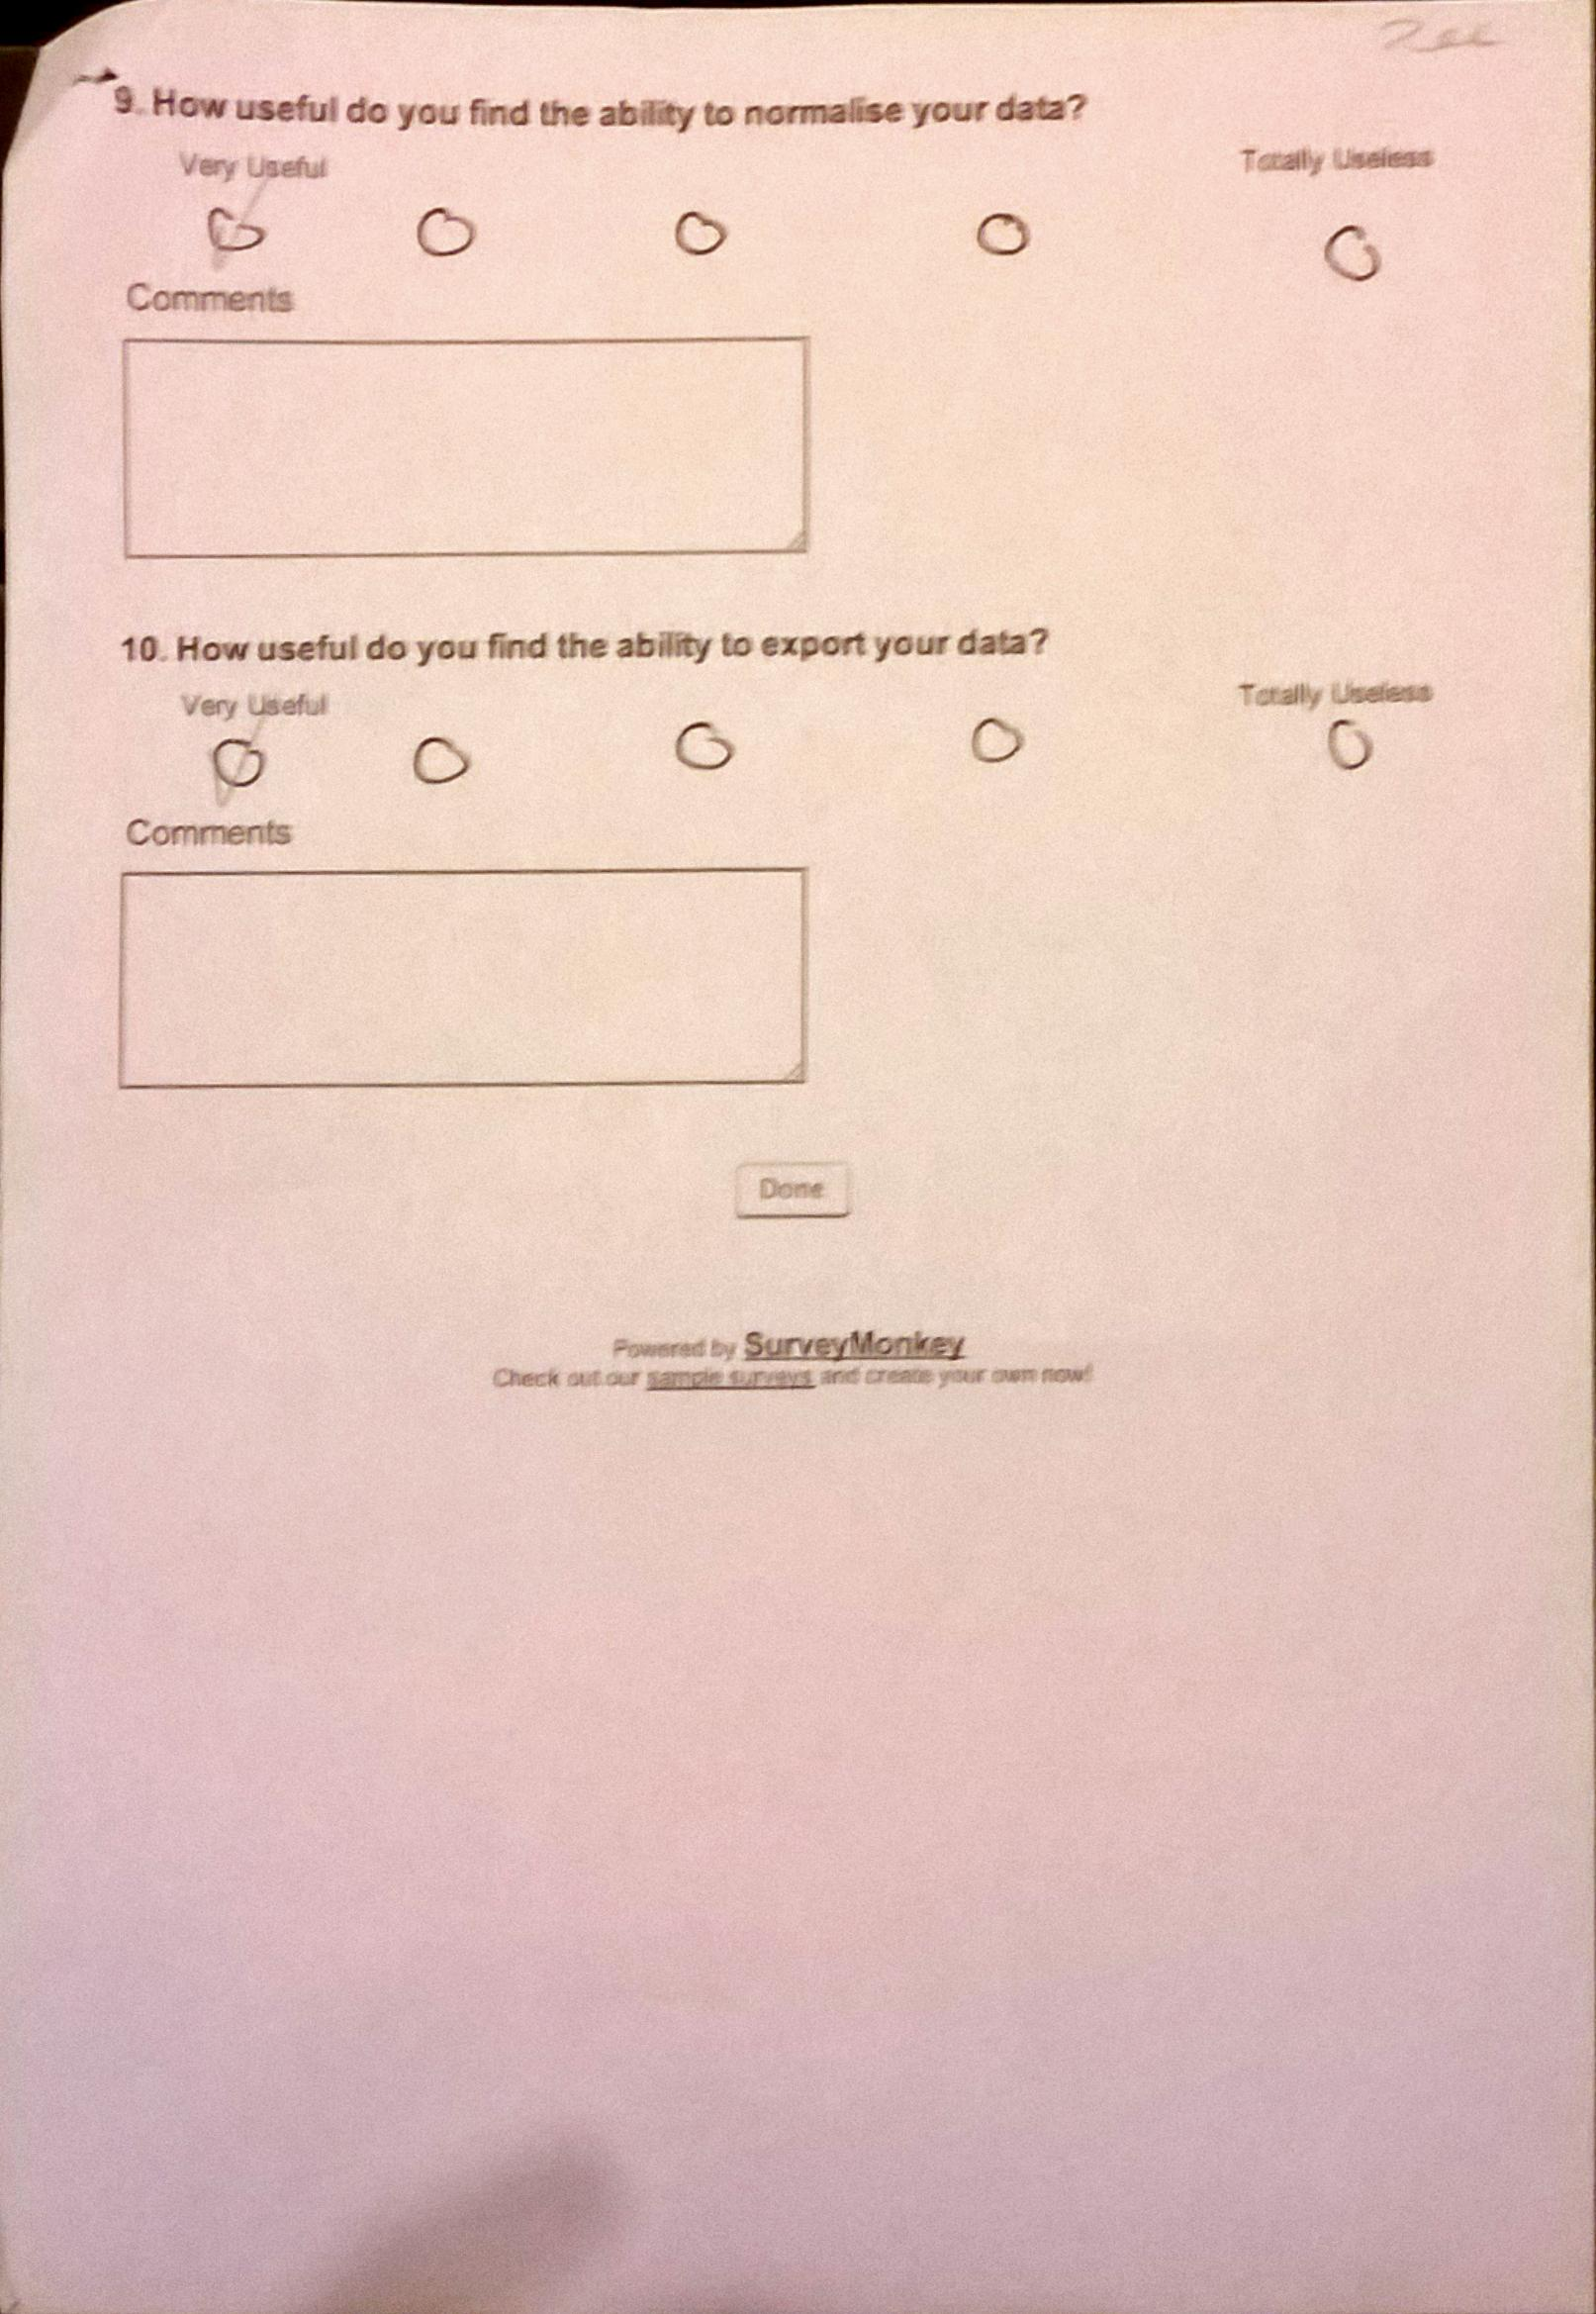
\includegraphics[width=0.95\textwidth]{images/user_eval/user_eval_11.jpg}
    \caption{Second Evaluation}
\end{figure}

\begin{figure}[h!]
    \centering
    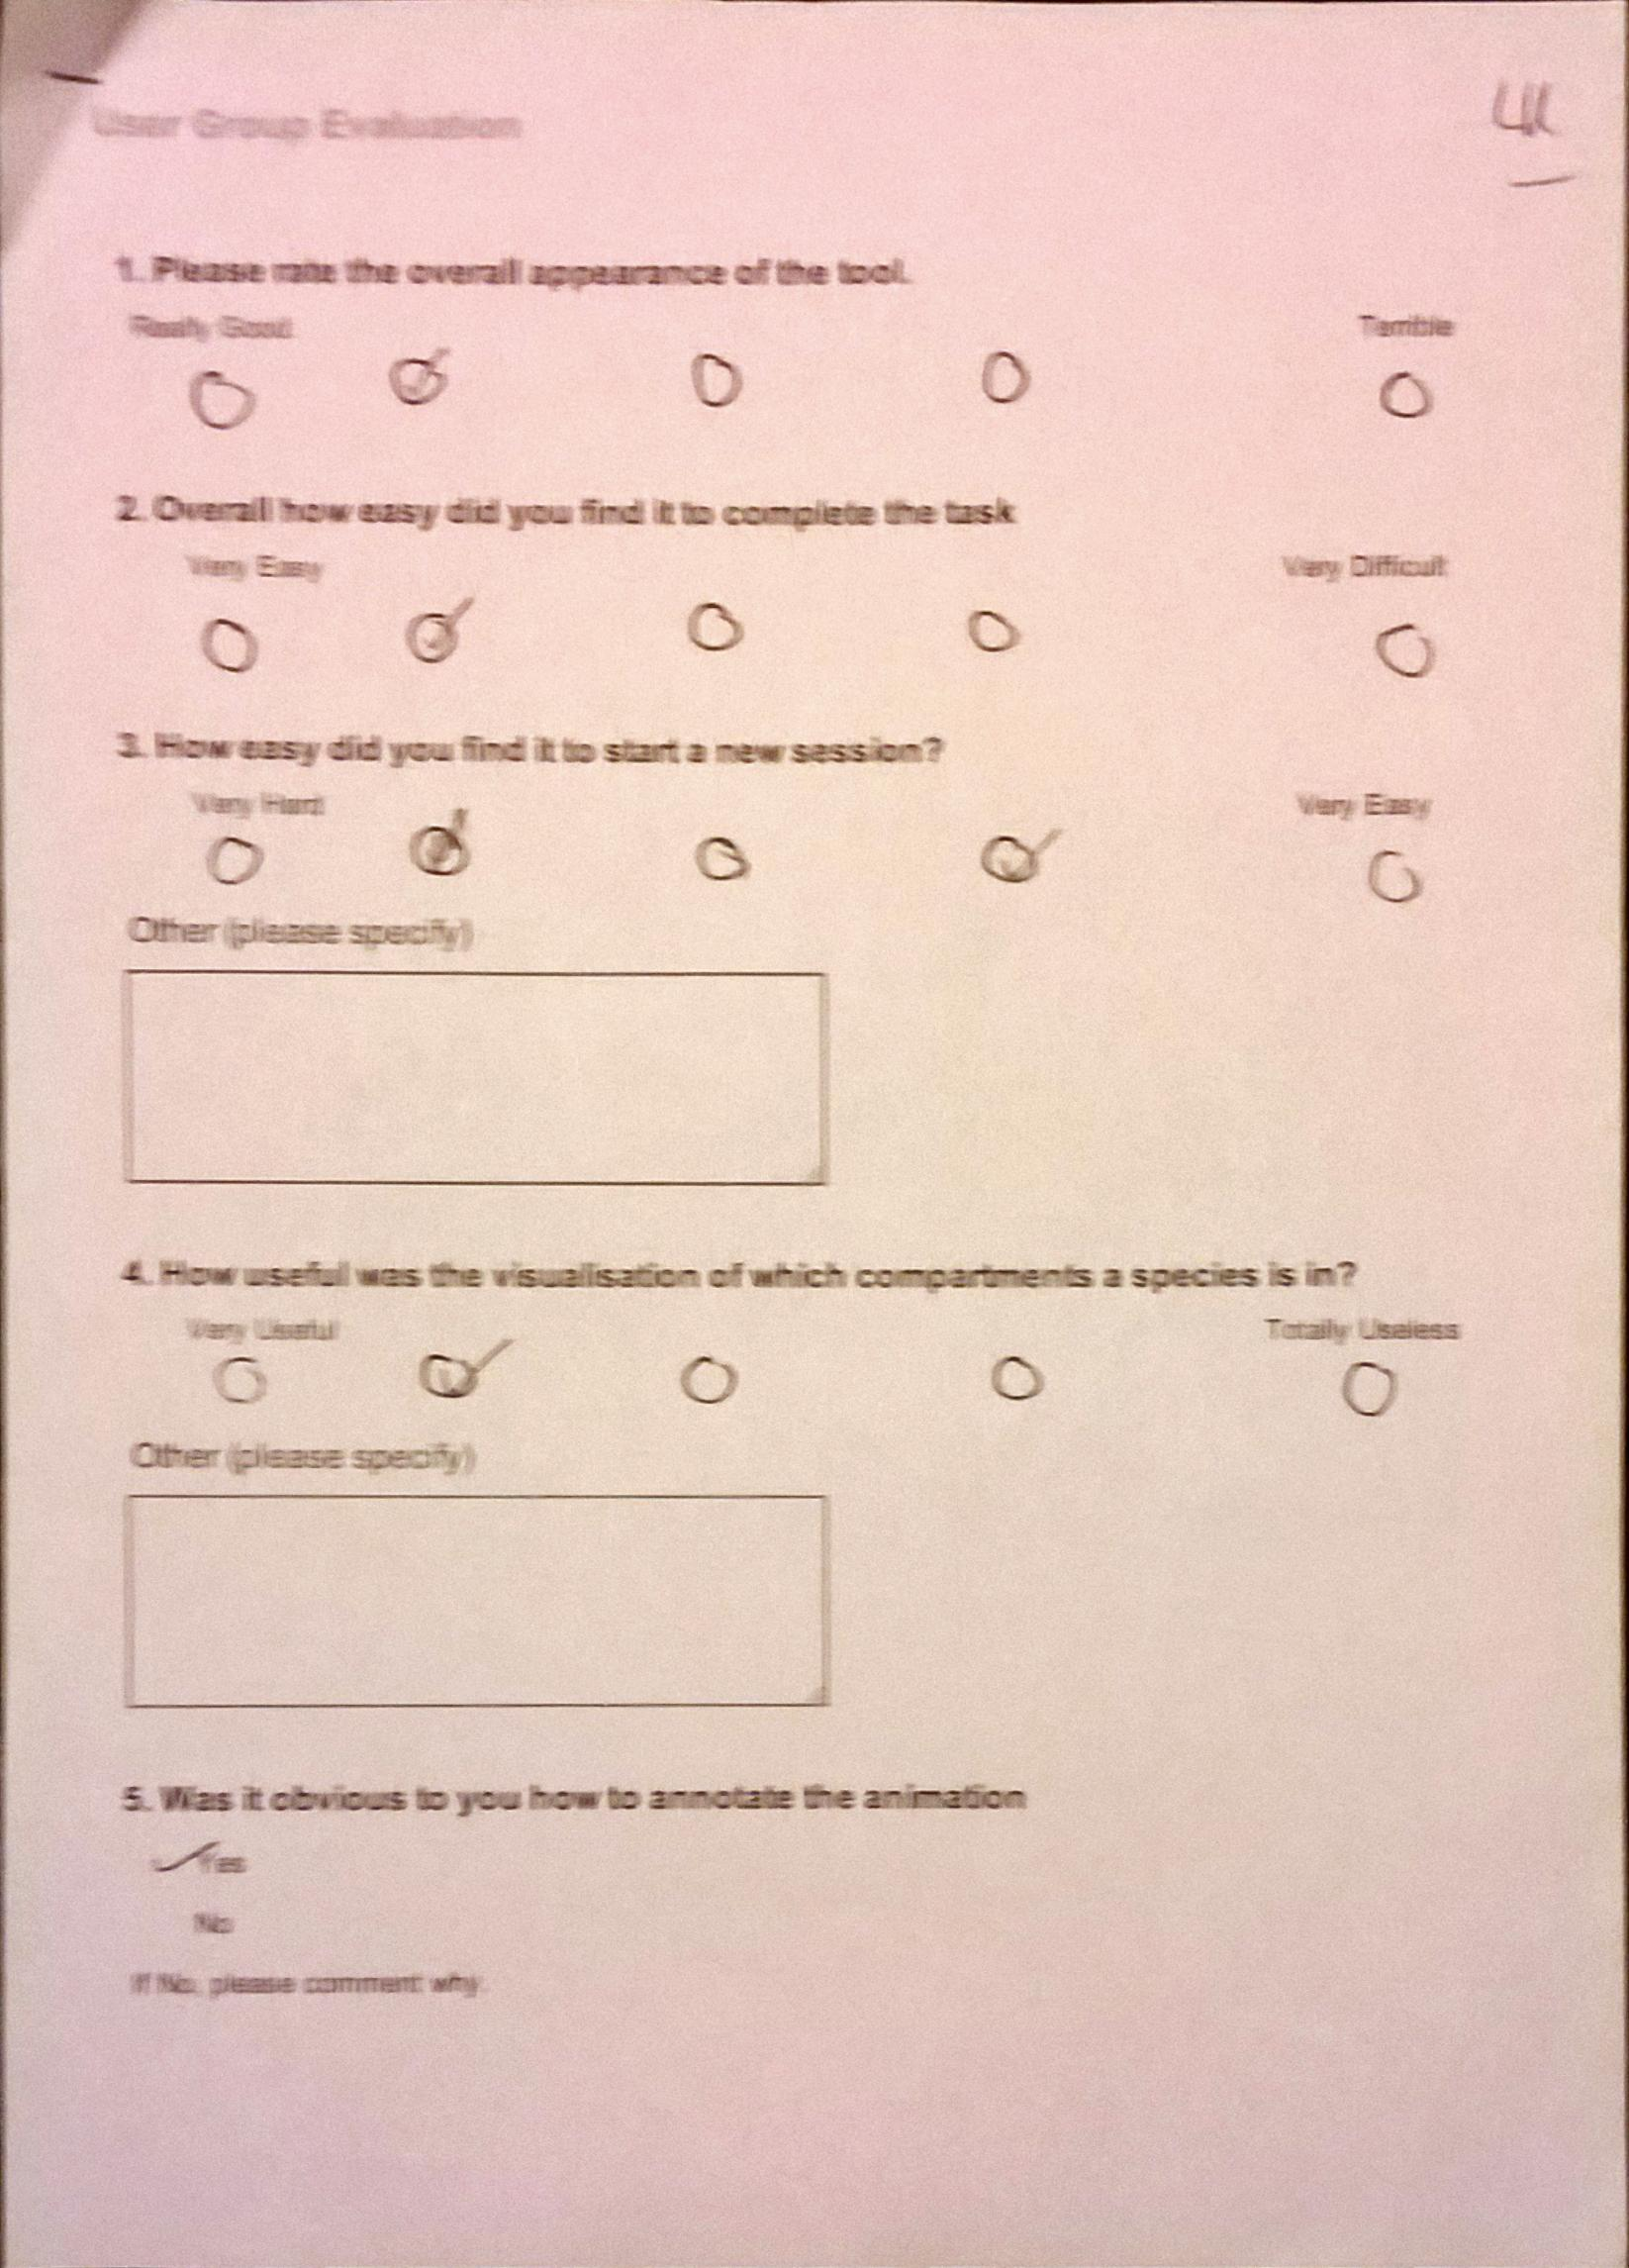
\includegraphics[width=0.95\textwidth]{images/user_eval/user_eval_12.jpg}
    \caption{Second Evaluation}
\end{figure}

\begin{figure}[h!]
    \centering
    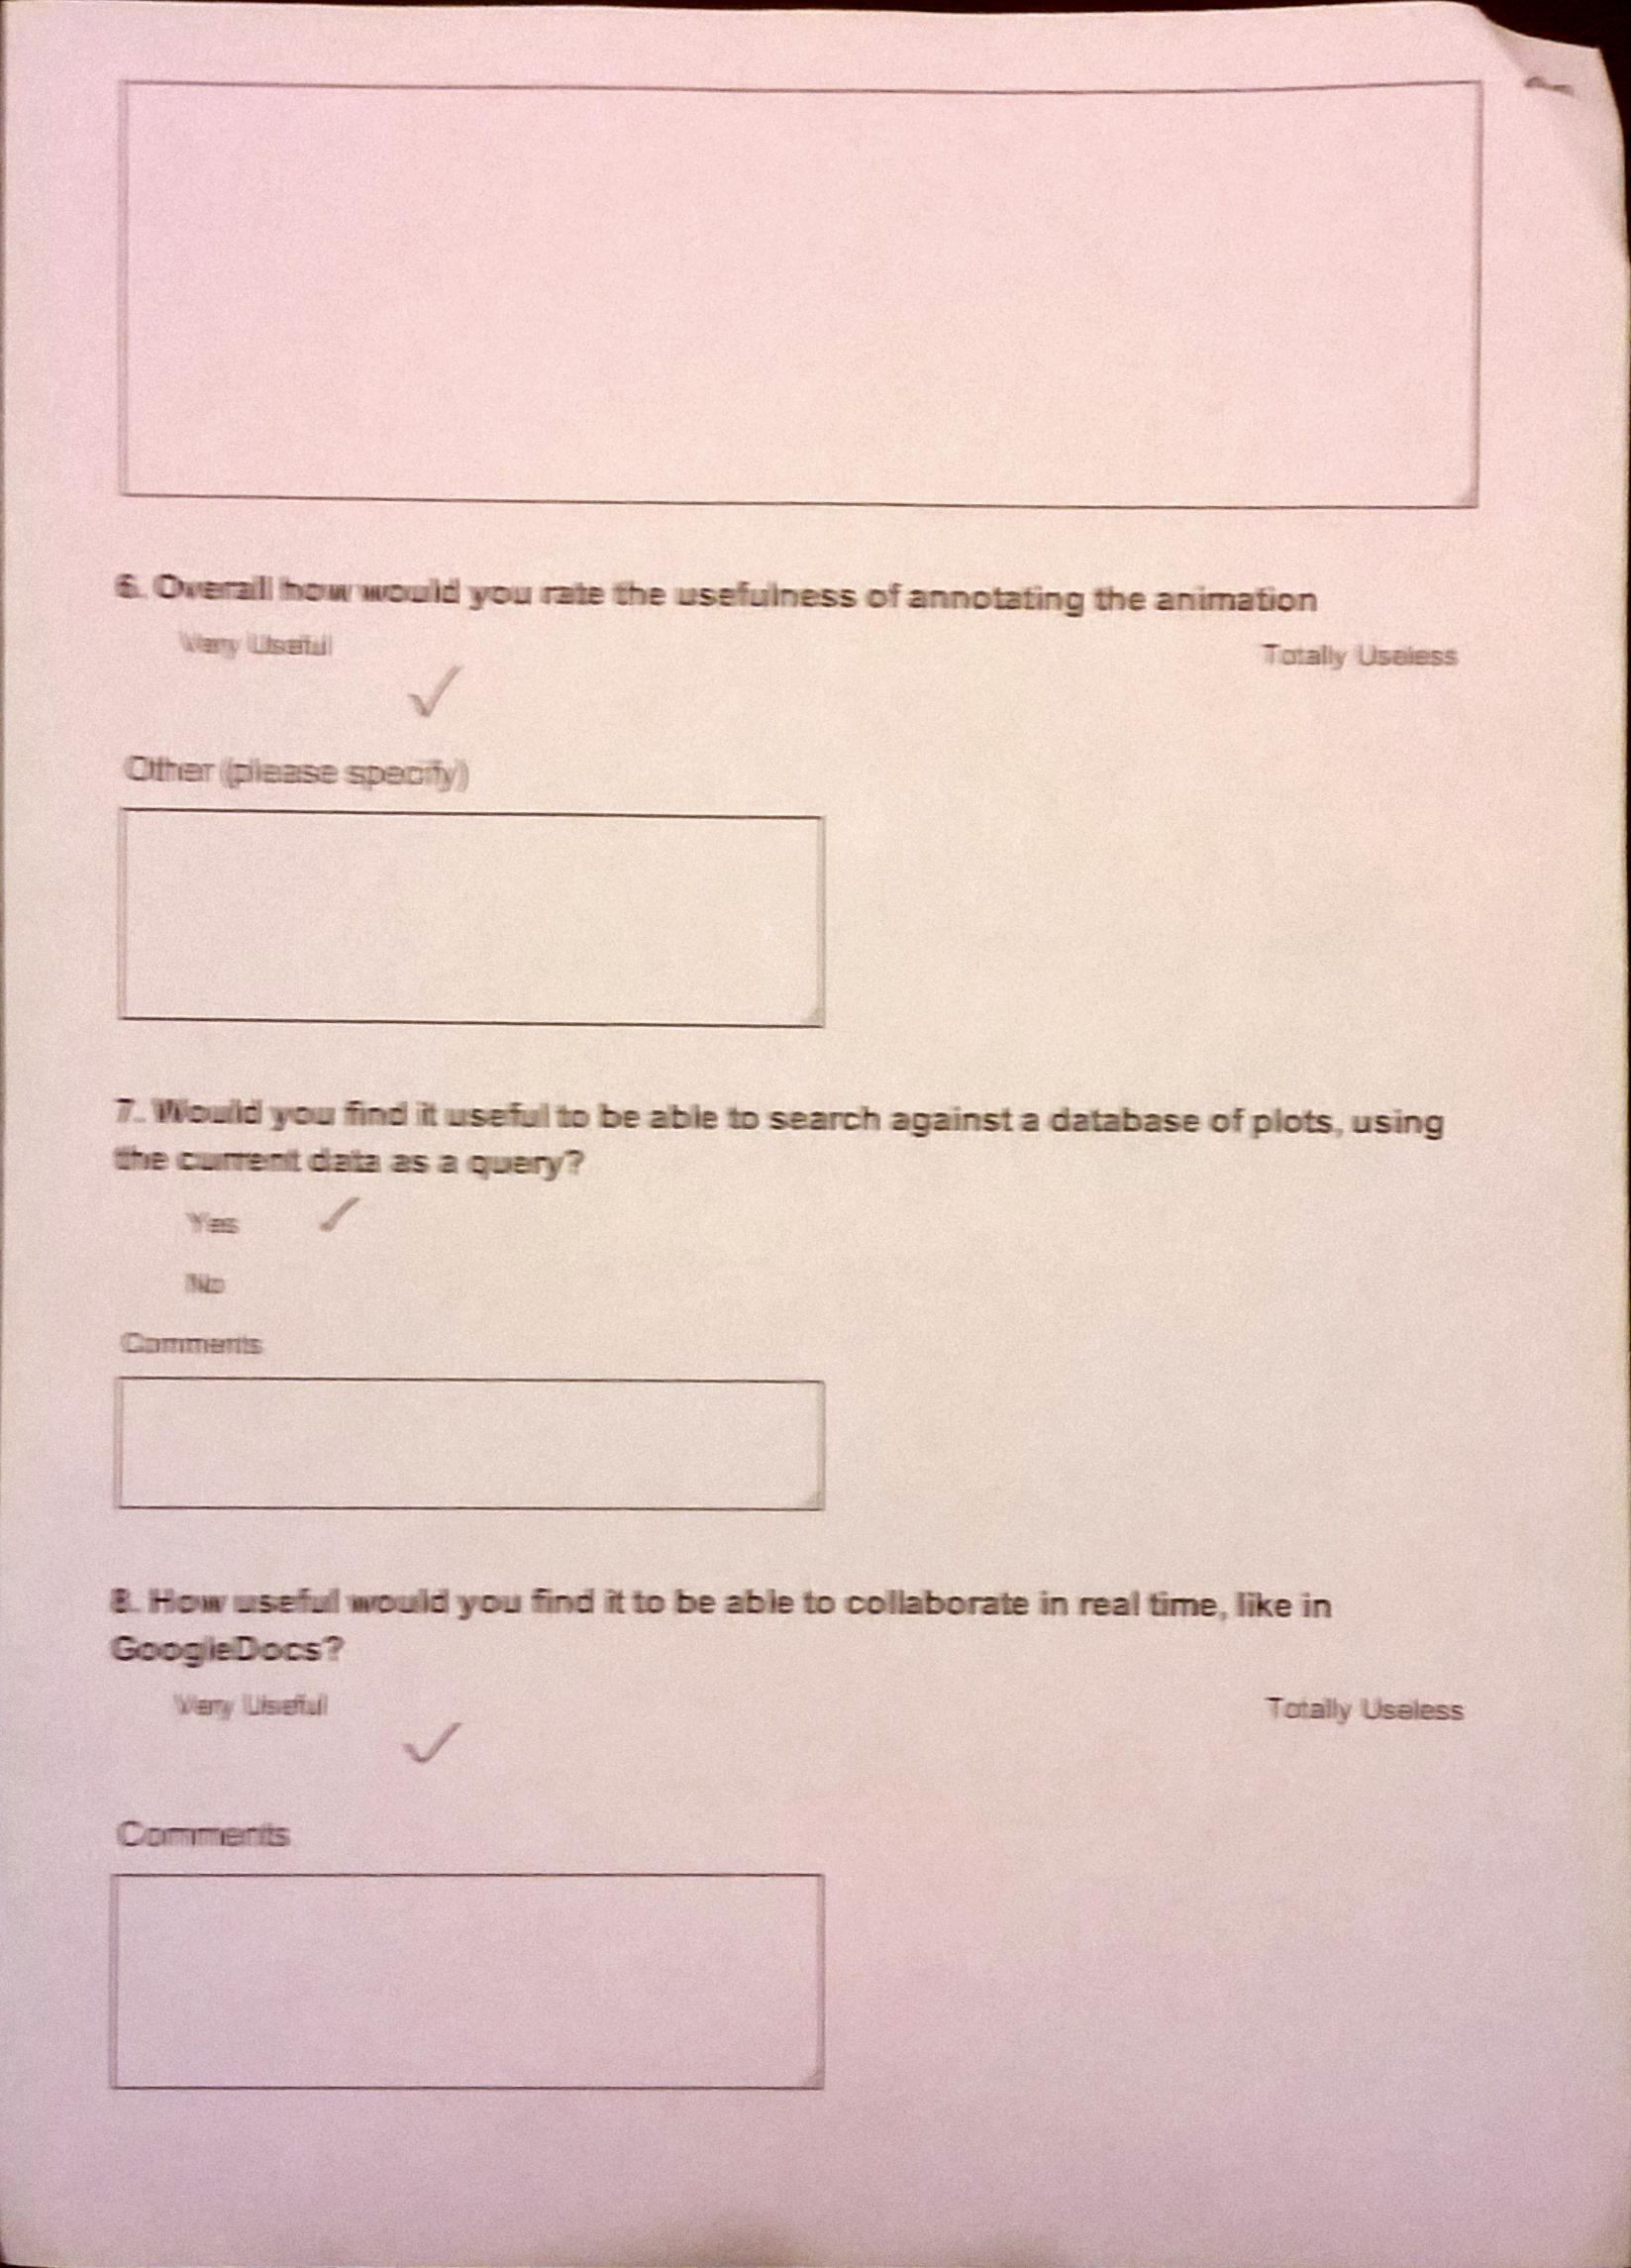
\includegraphics[width=0.95\textwidth]{images/user_eval/user_eval_13.jpg}
    \caption{Second Evaluation}
\end{figure}

\begin{figure}[h!]
    \centering
    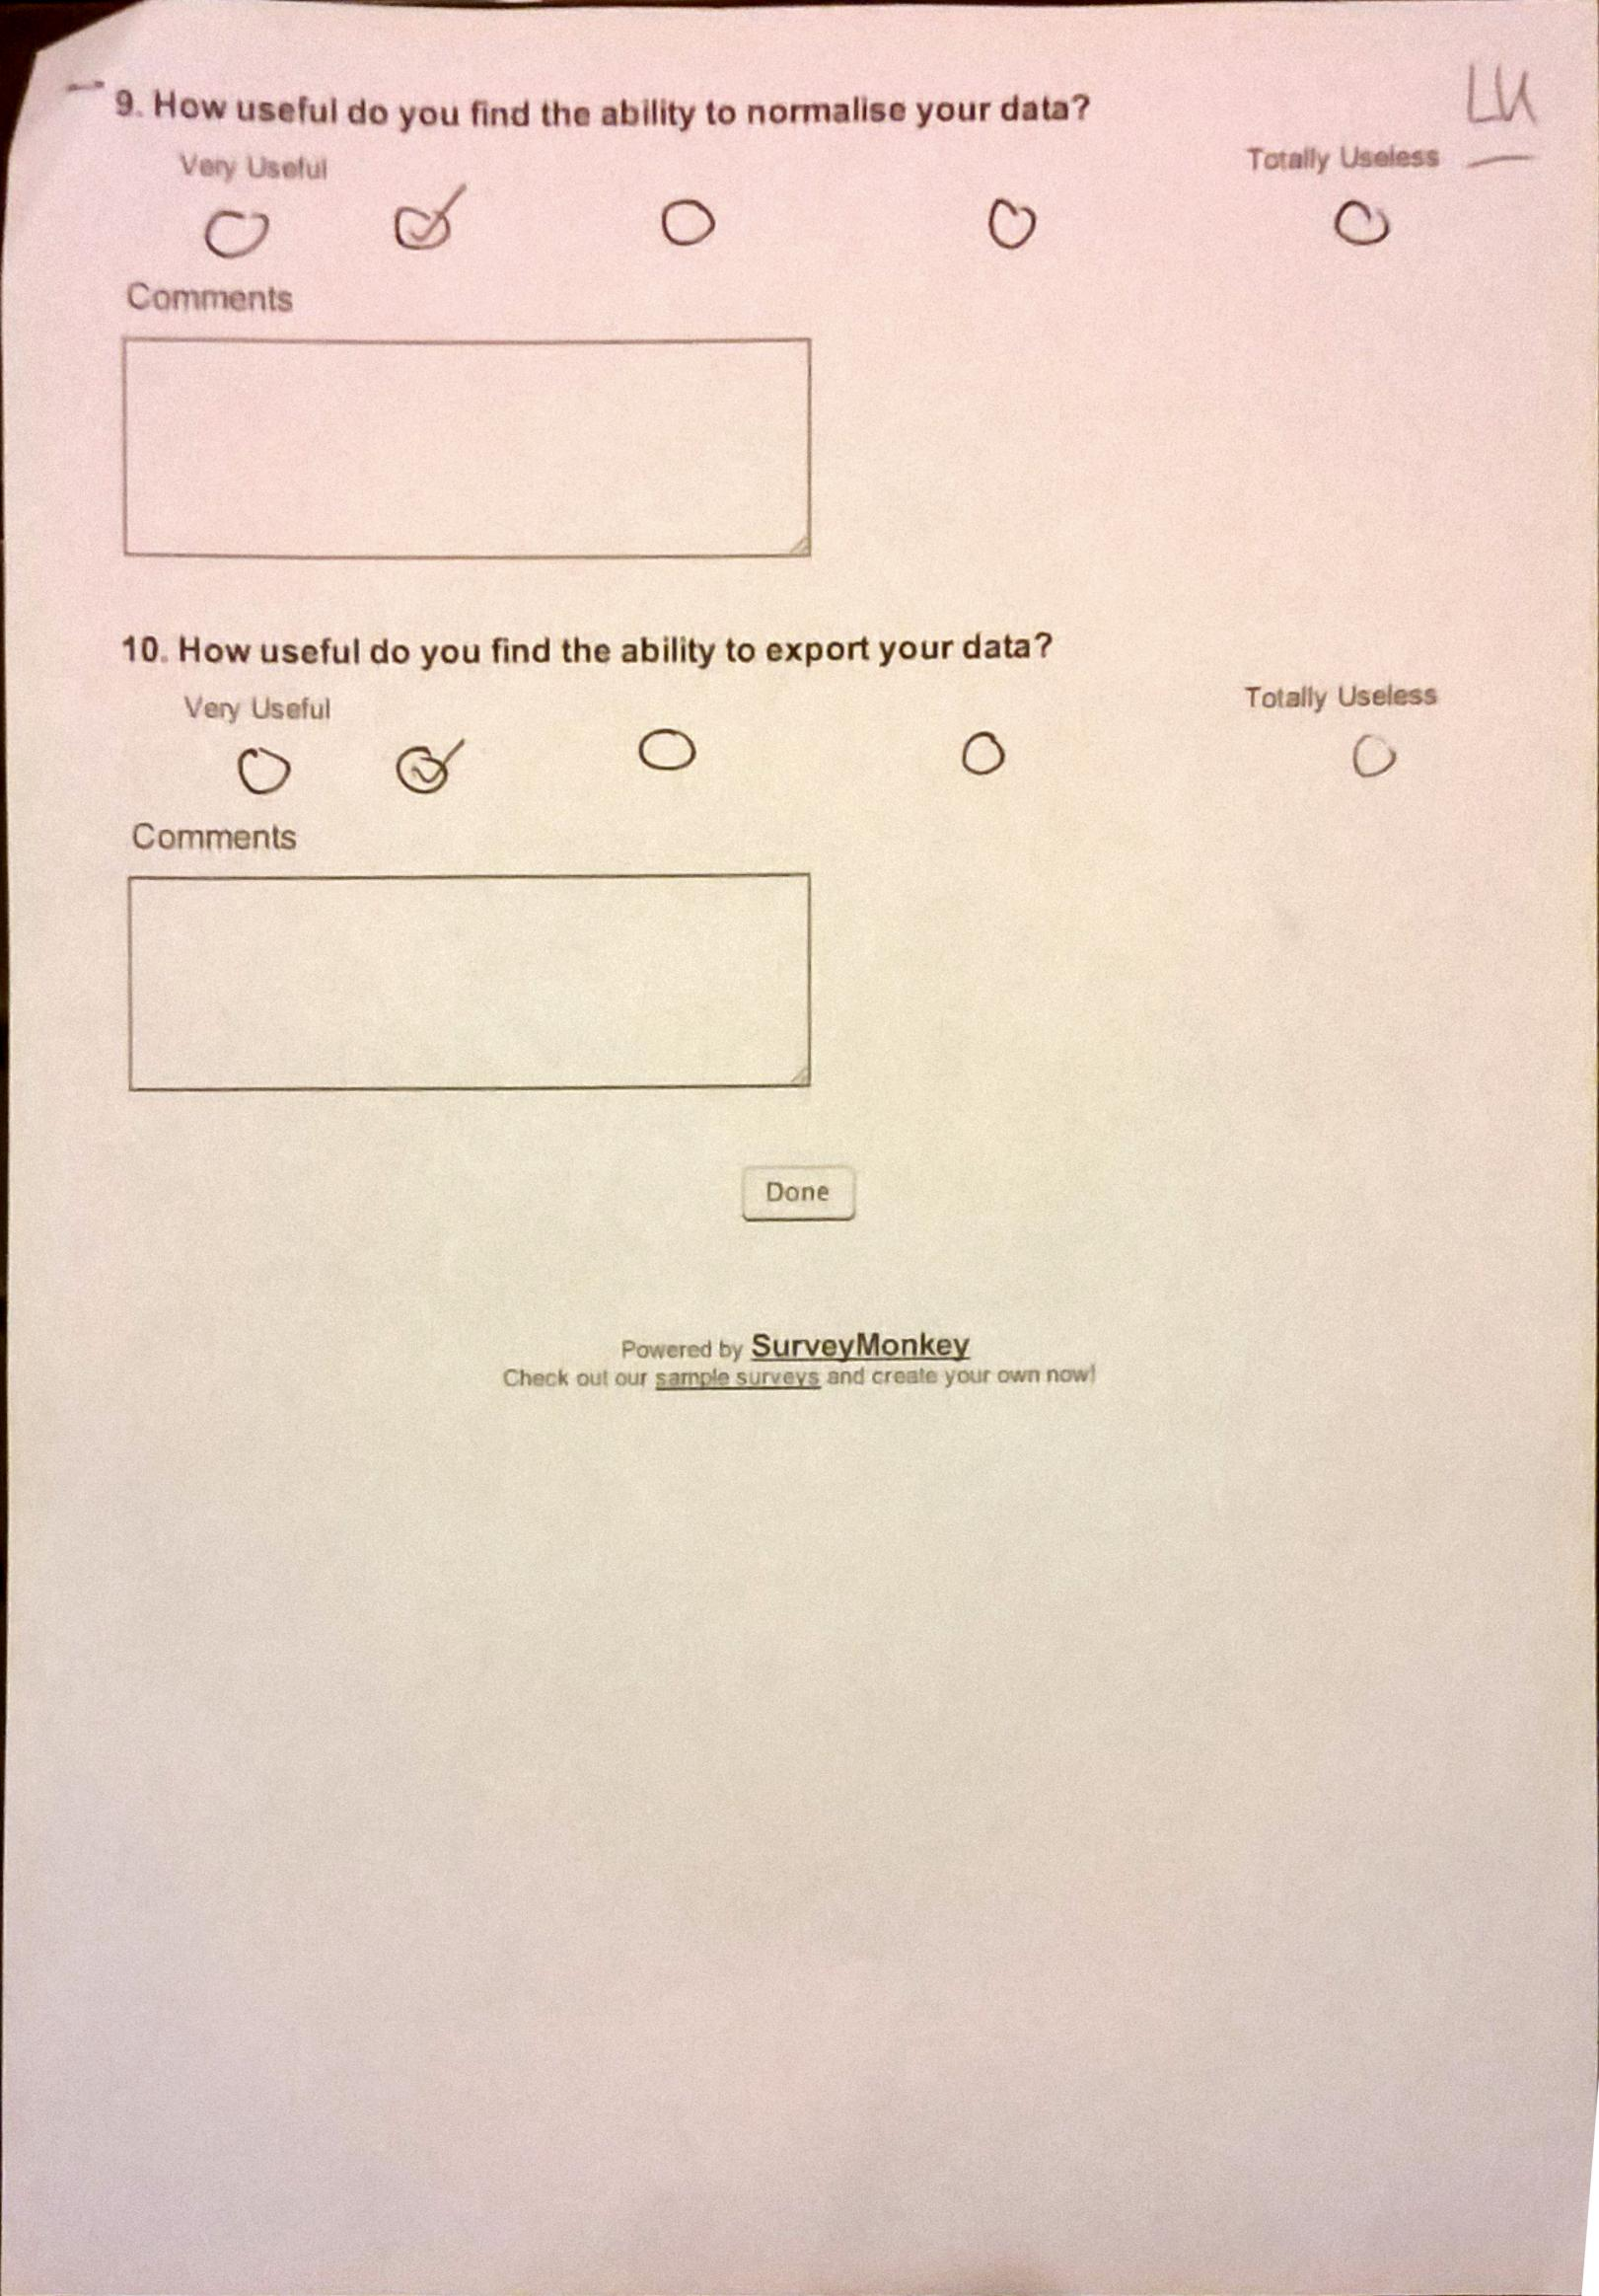
\includegraphics[width=0.95\textwidth]{images/user_eval/user_eval_14.jpg}
    \caption{Second Evaluation}
\end{figure}

\begin{figure}[h!]
    \centering
    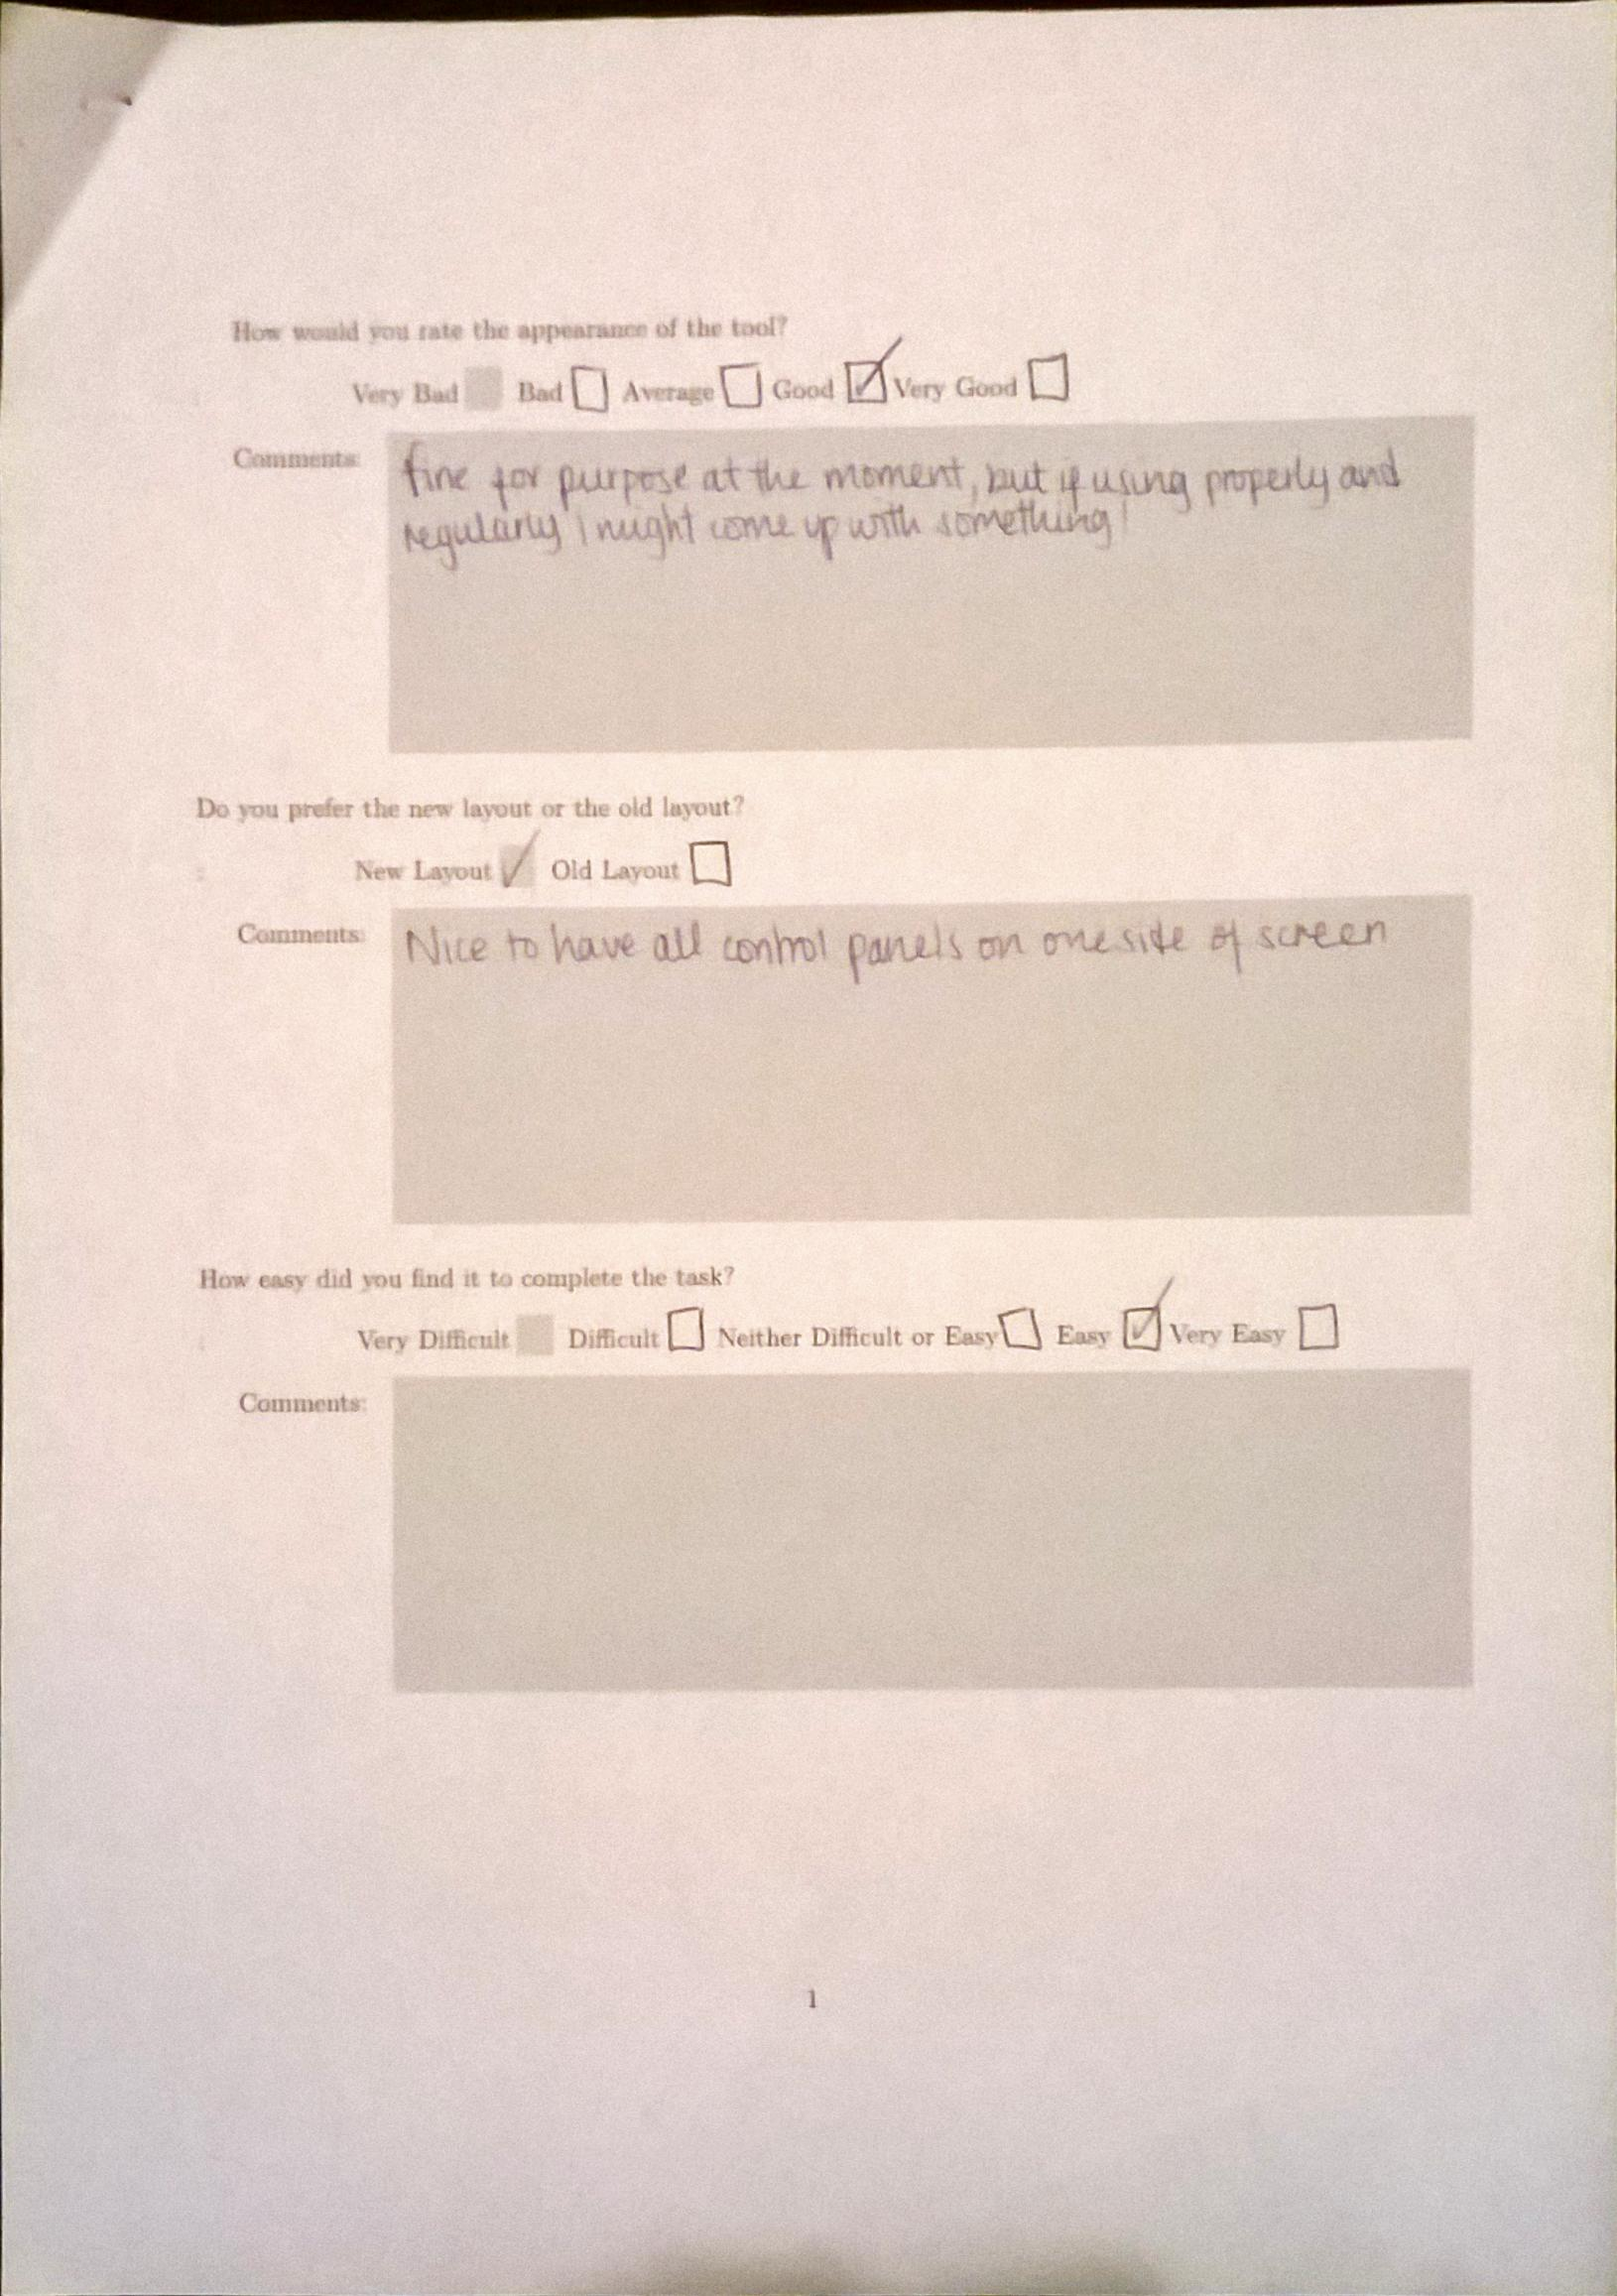
\includegraphics[width=0.95\textwidth]{images/user_eval/user_eval_15.jpg}
    \caption{Third Evaluation}
\end{figure}

\begin{figure}[h!]
    \centering
    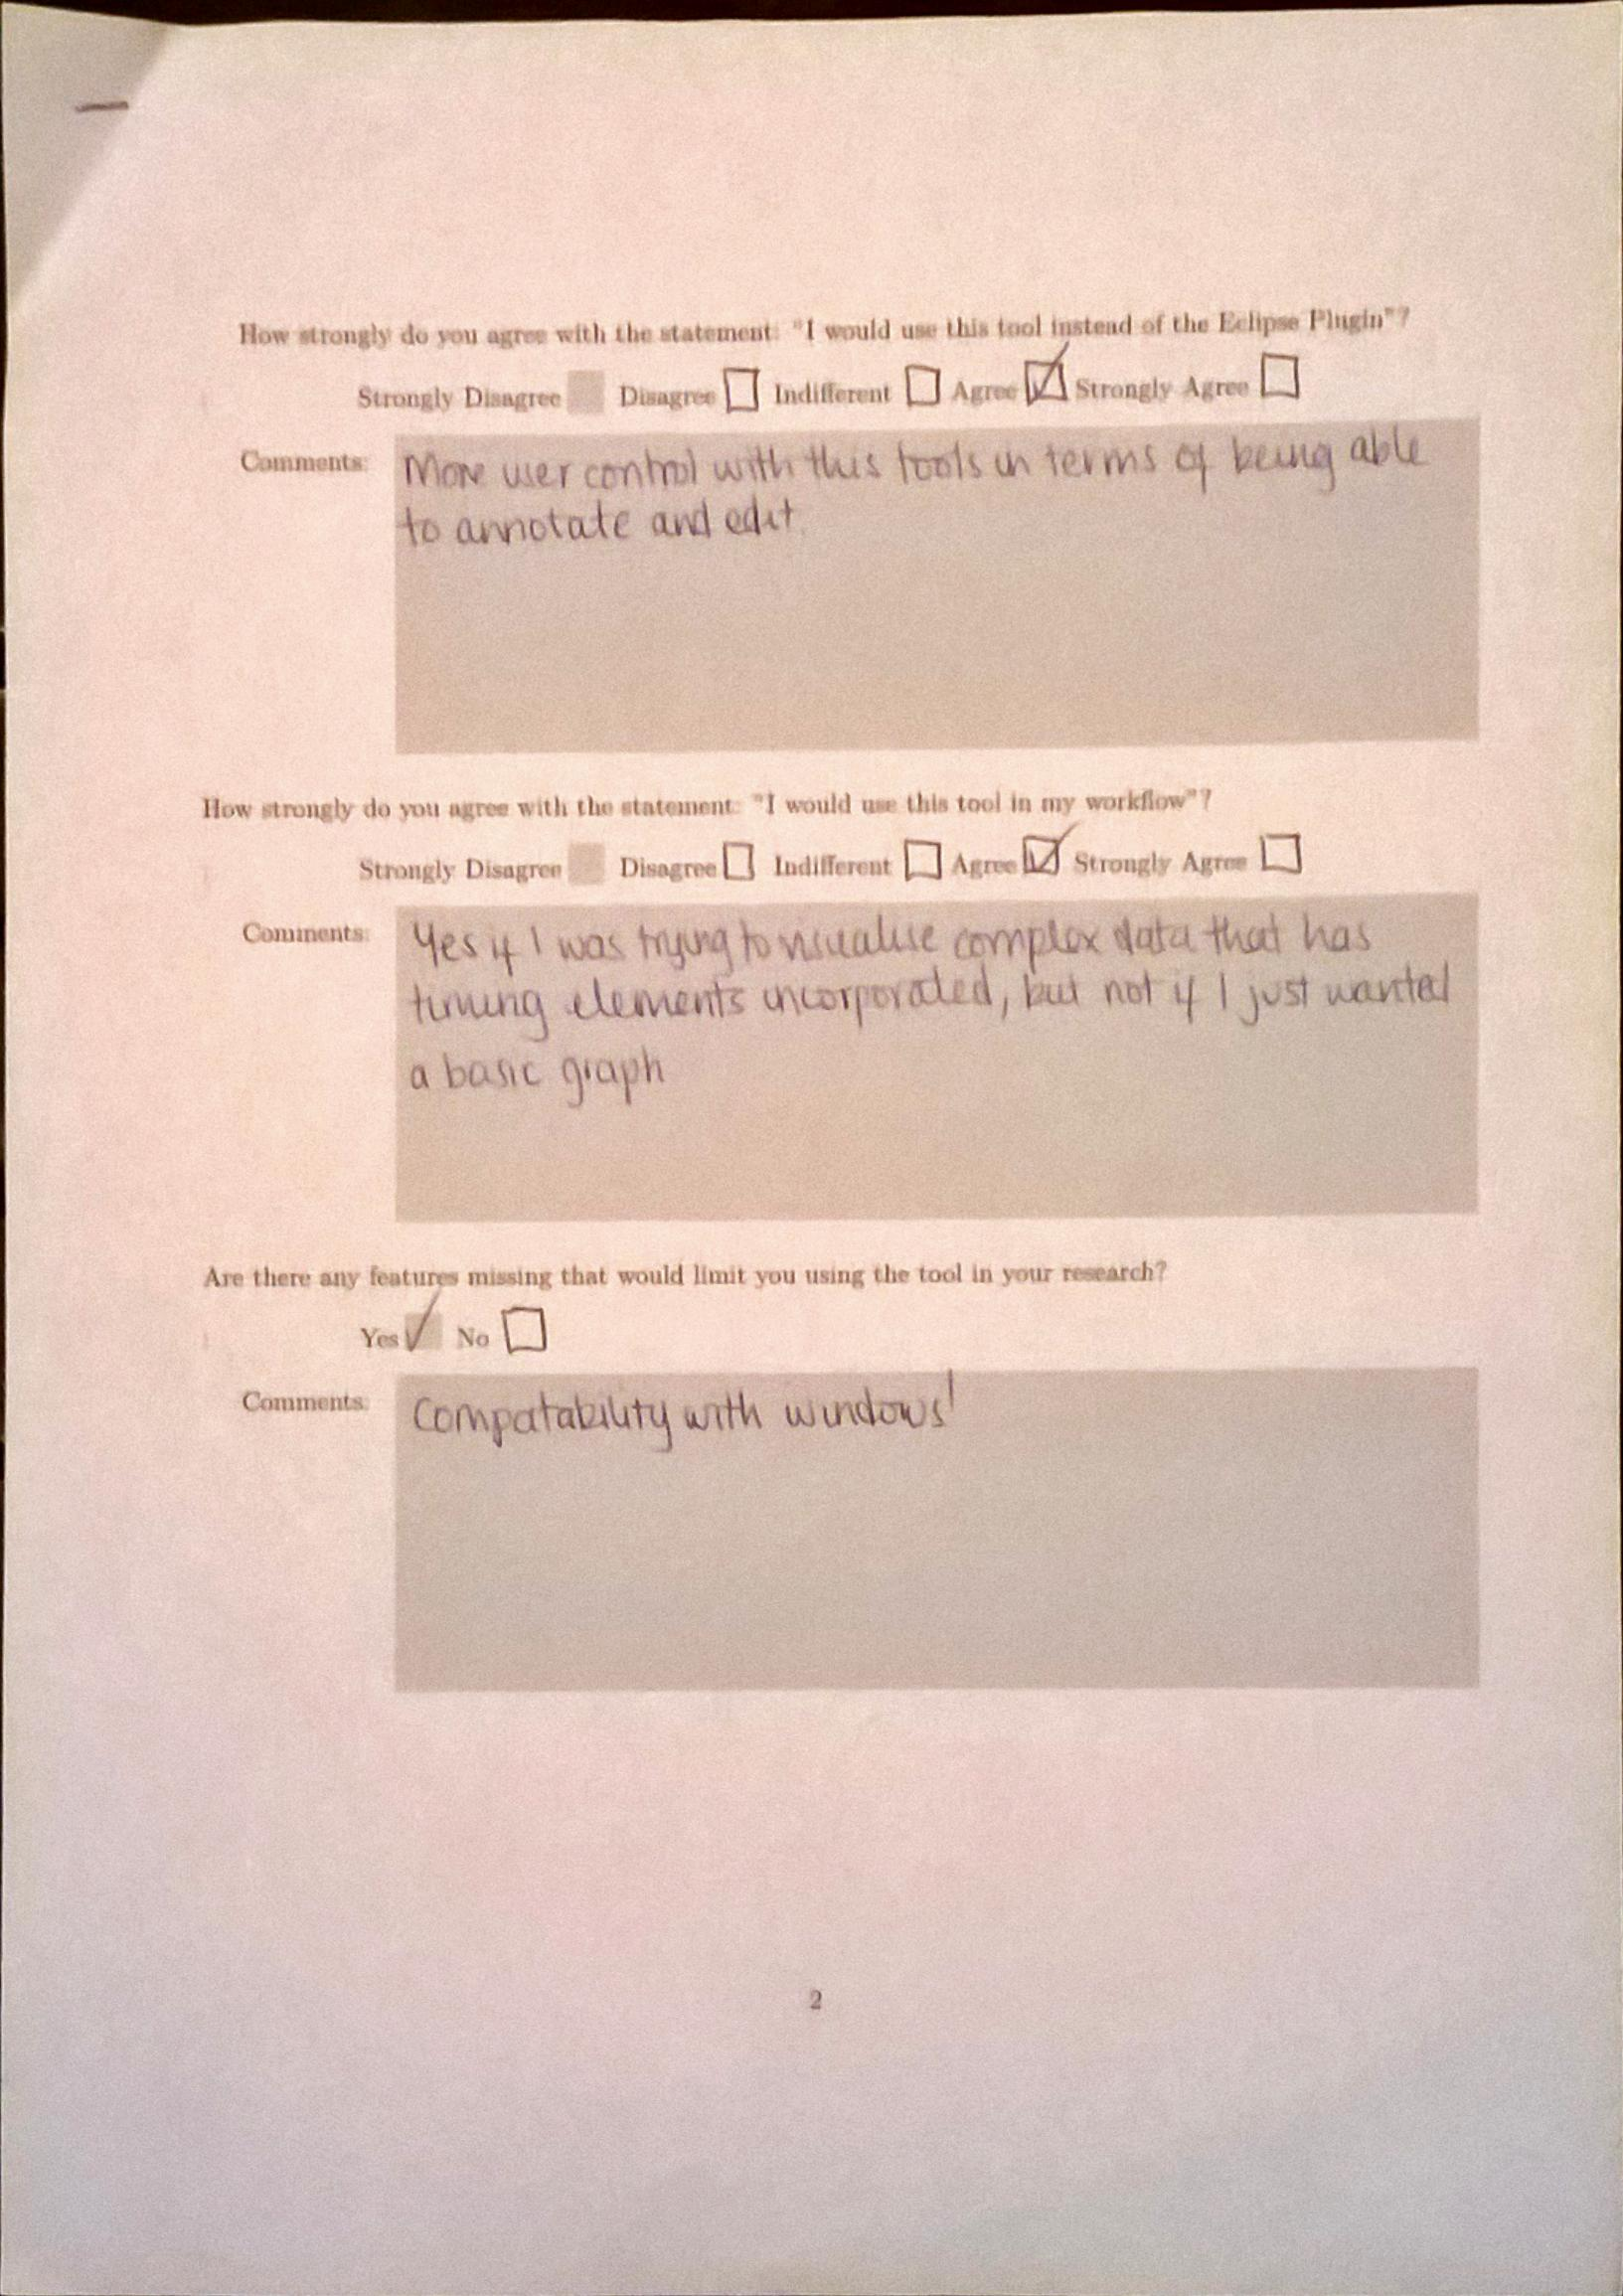
\includegraphics[width=0.95\textwidth]{images/user_eval/user_eval_16.jpg}
    \caption{Third Evaluation}
\end{figure}

\begin{figure}[h!]
    \centering
    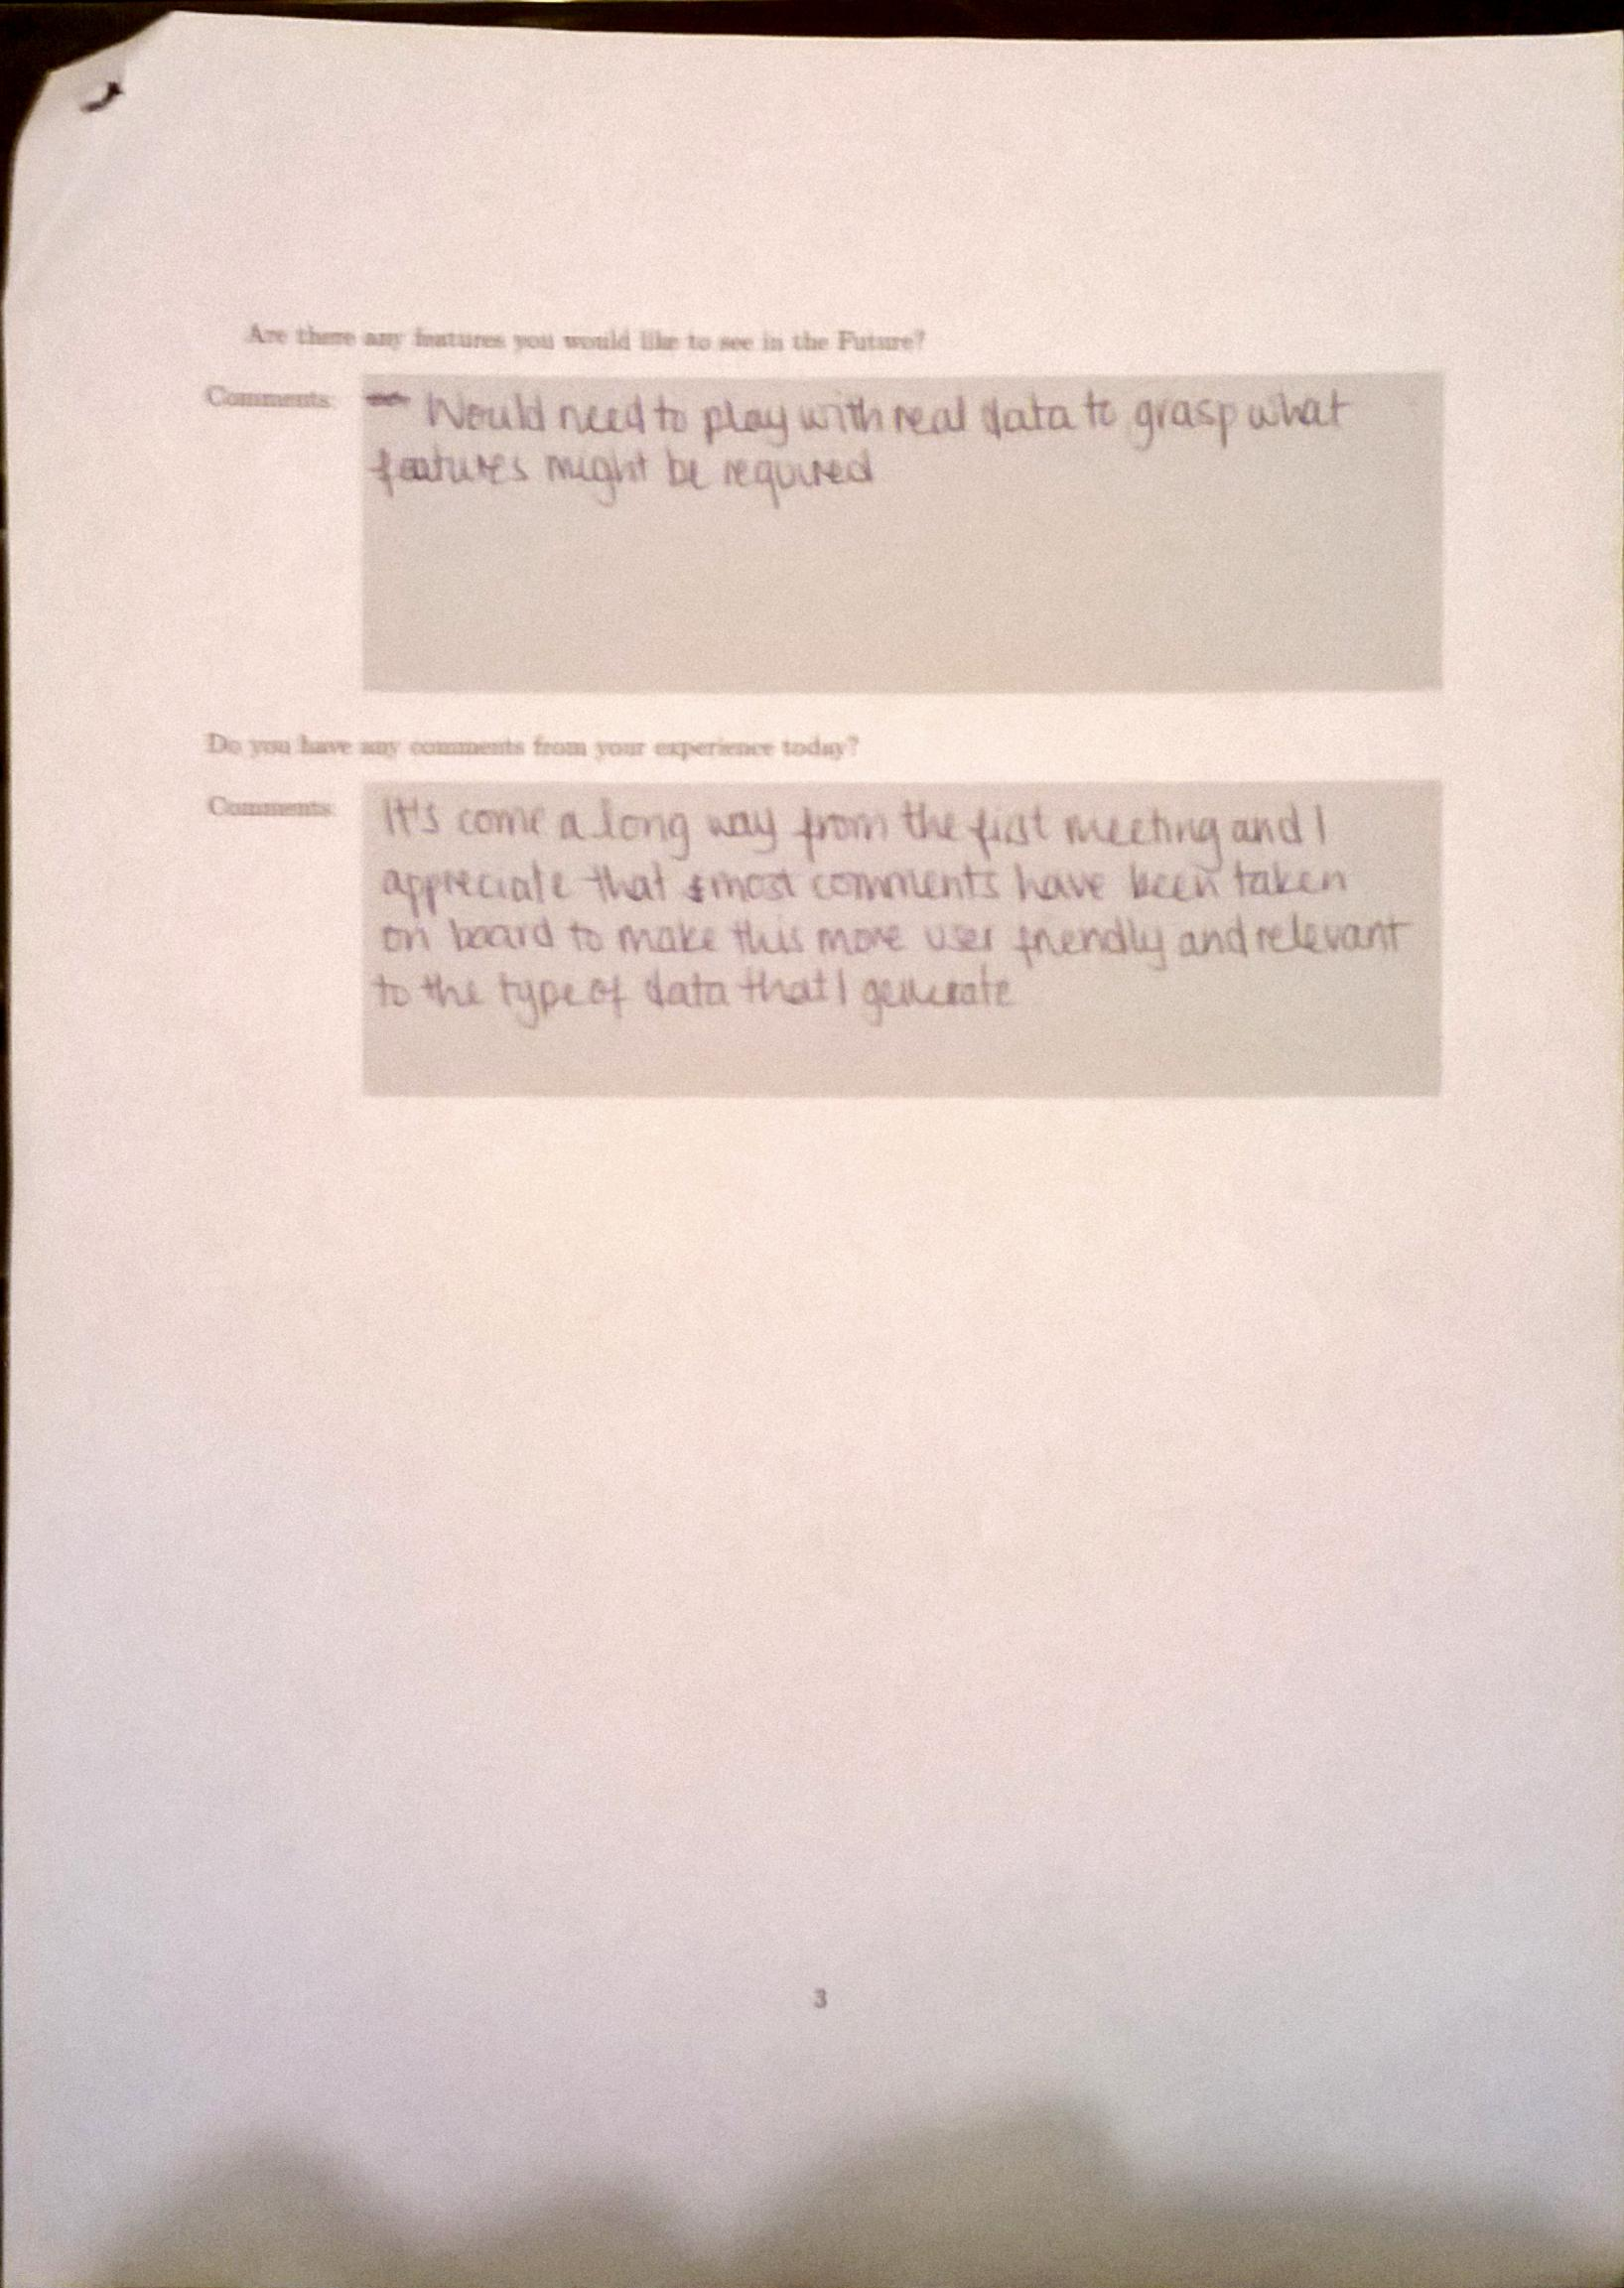
\includegraphics[width=0.95\textwidth]{images/user_eval/user_eval_17.jpg}
    \caption{Third Evaluation}
\end{figure}

\begin{figure}[h!]
    \centering
    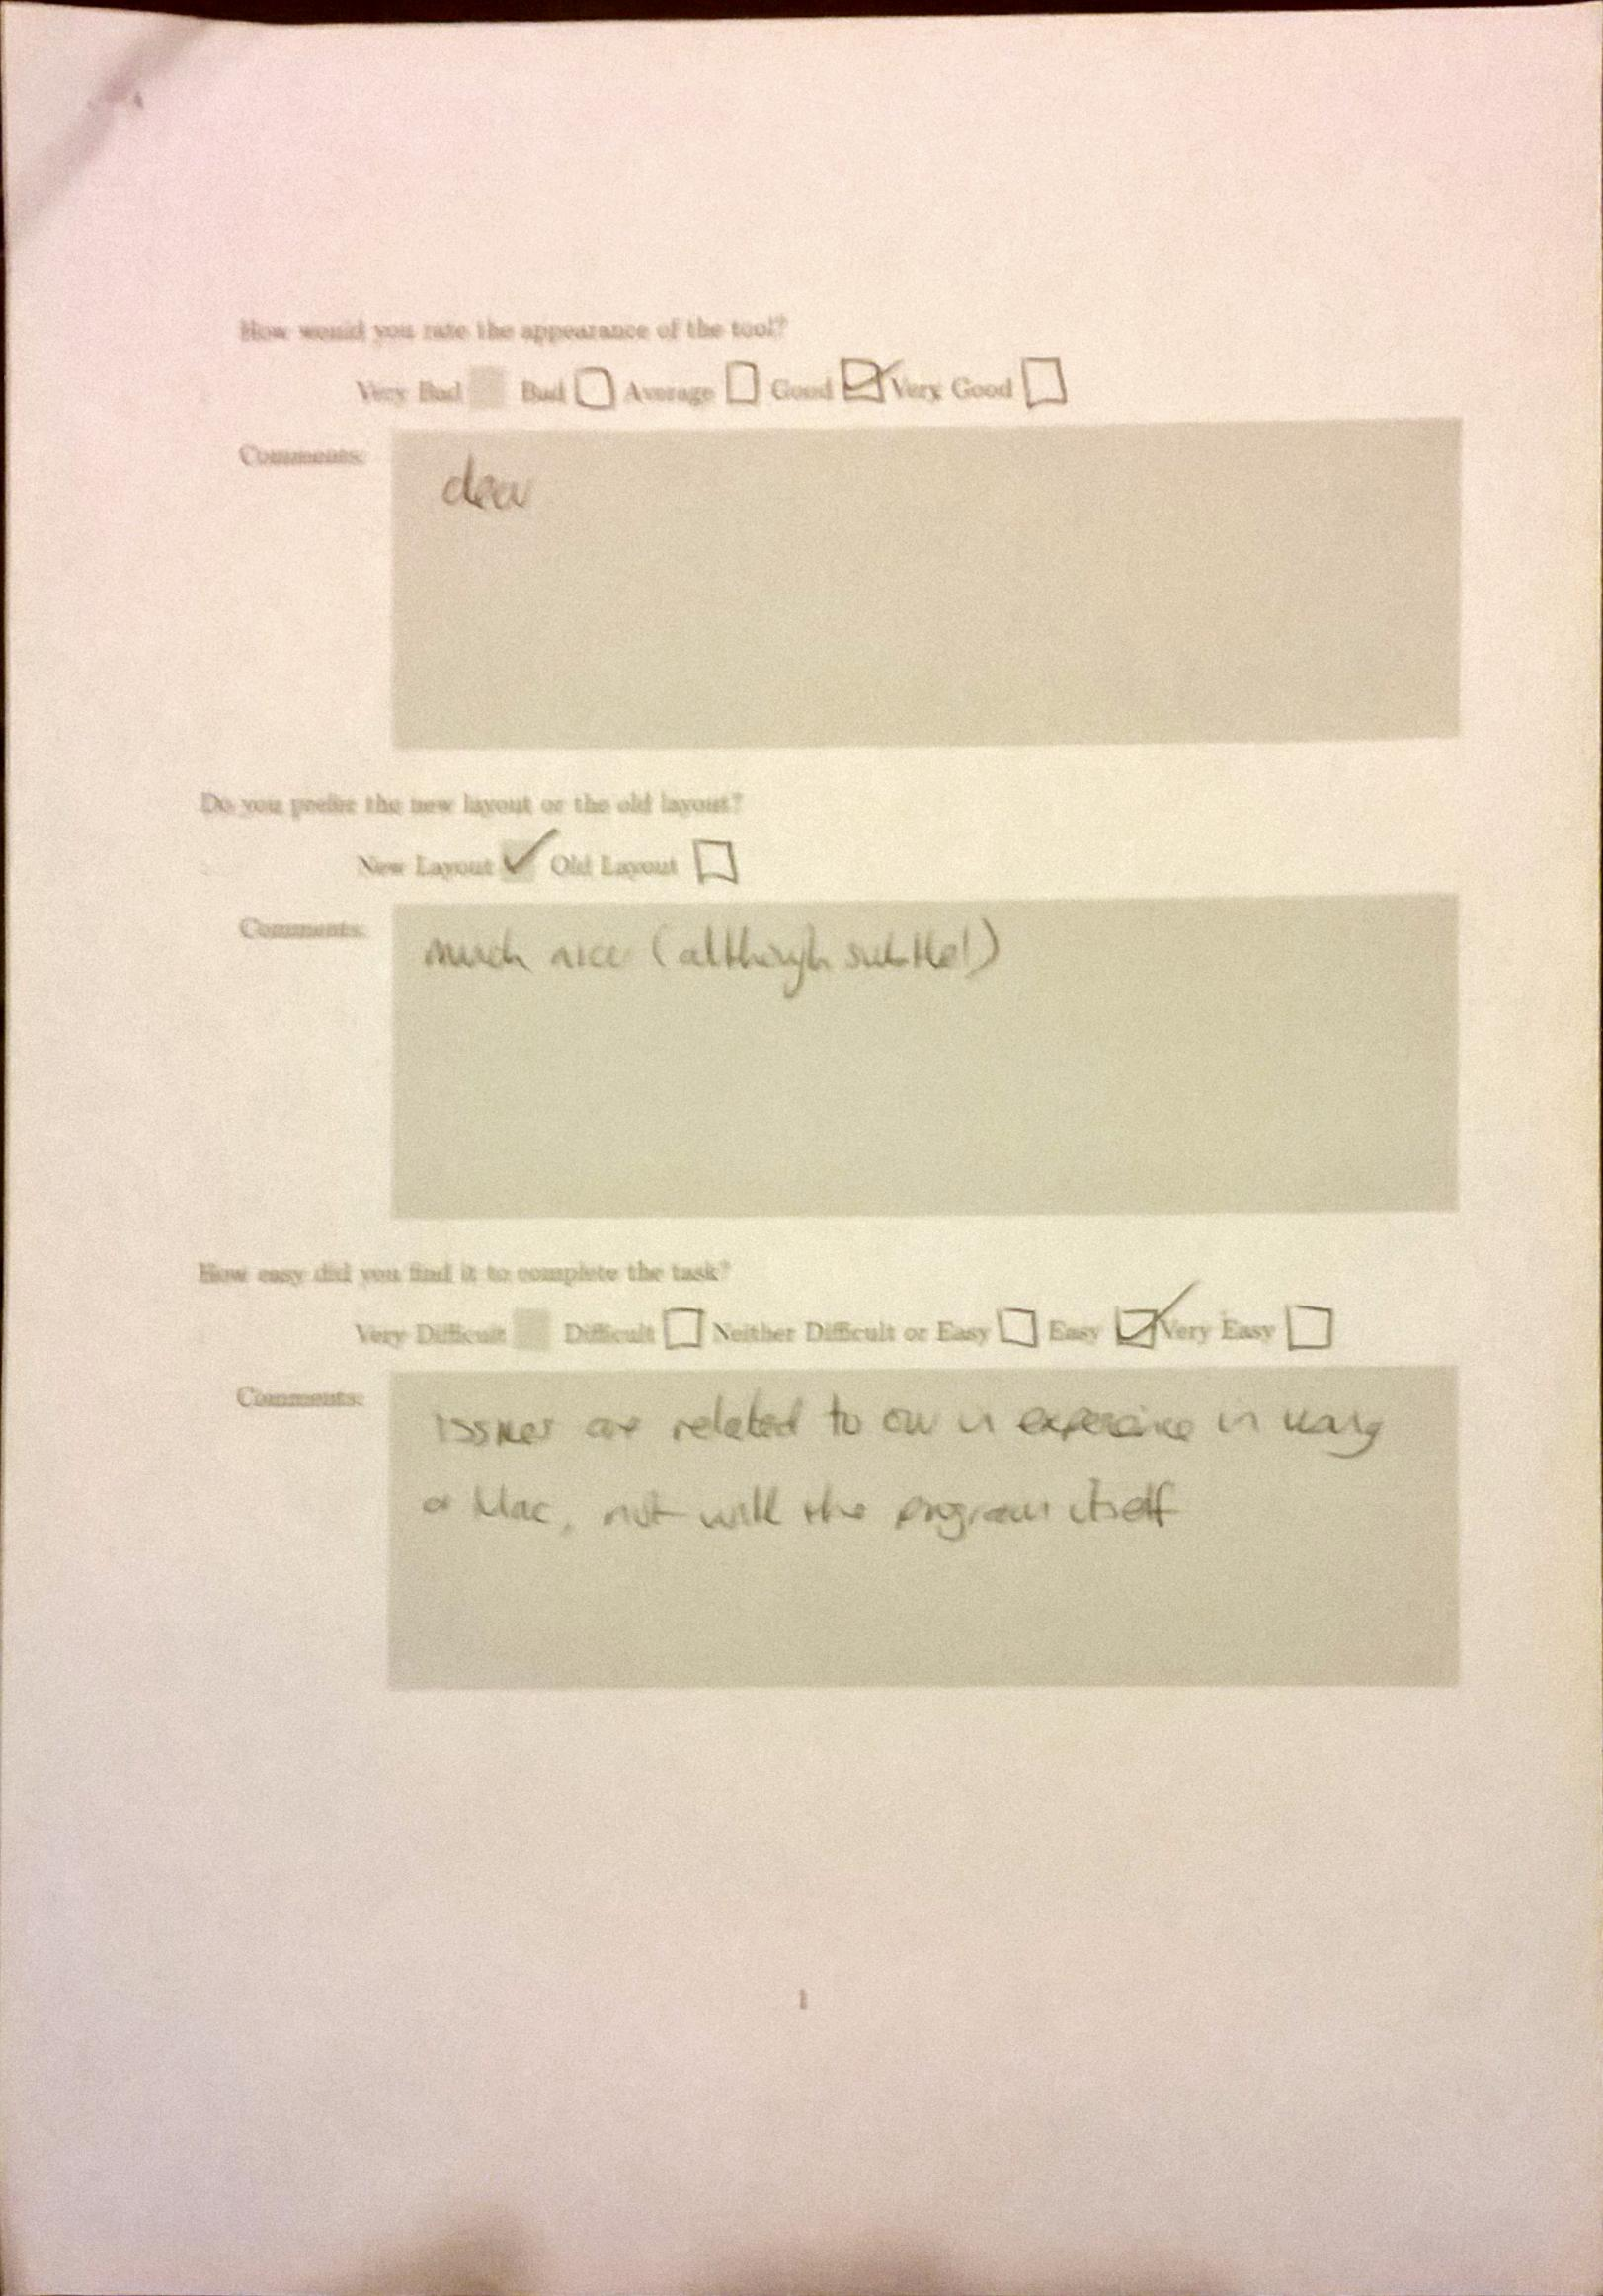
\includegraphics[width=0.95\textwidth]{images/user_eval/user_eval_18.jpg}
    \caption{Third Evaluation}
\end{figure}

\begin{figure}[h!]
    \centering
    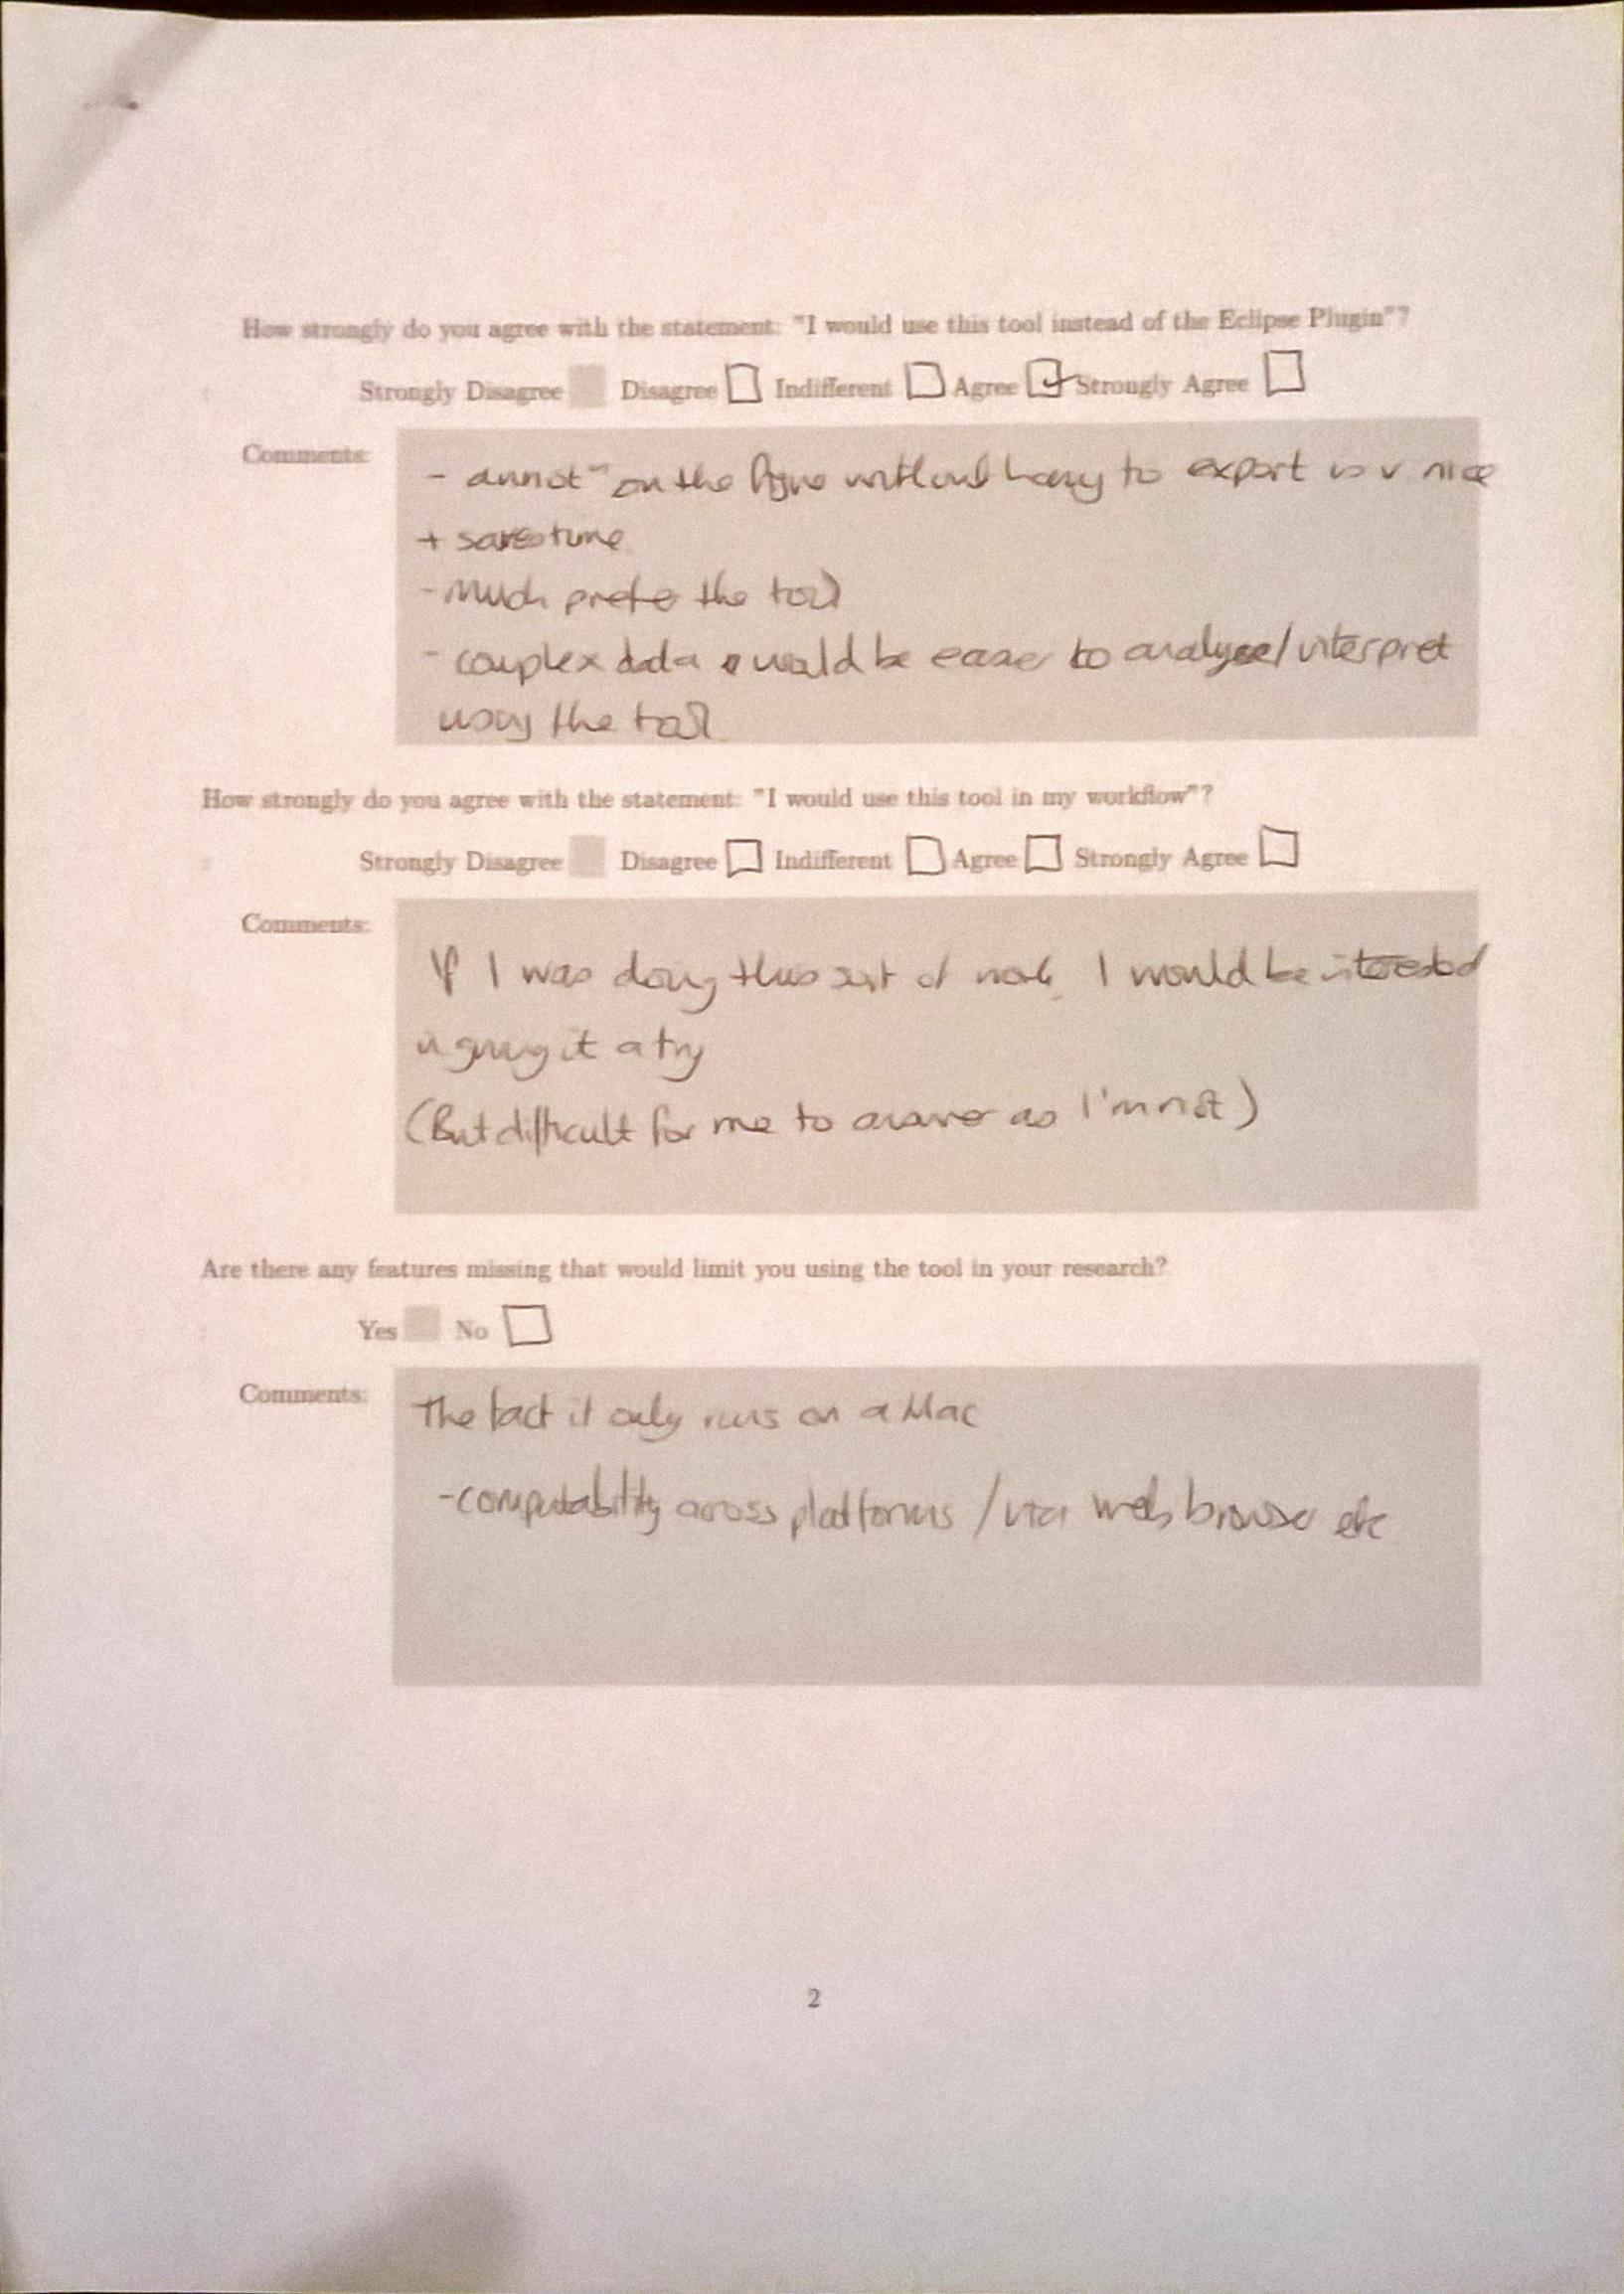
\includegraphics[width=0.95\textwidth]{images/user_eval/user_eval_19.jpg}
    \caption{Third Evaluation}
\end{figure}

\begin{figure}[h!]
    \centering
    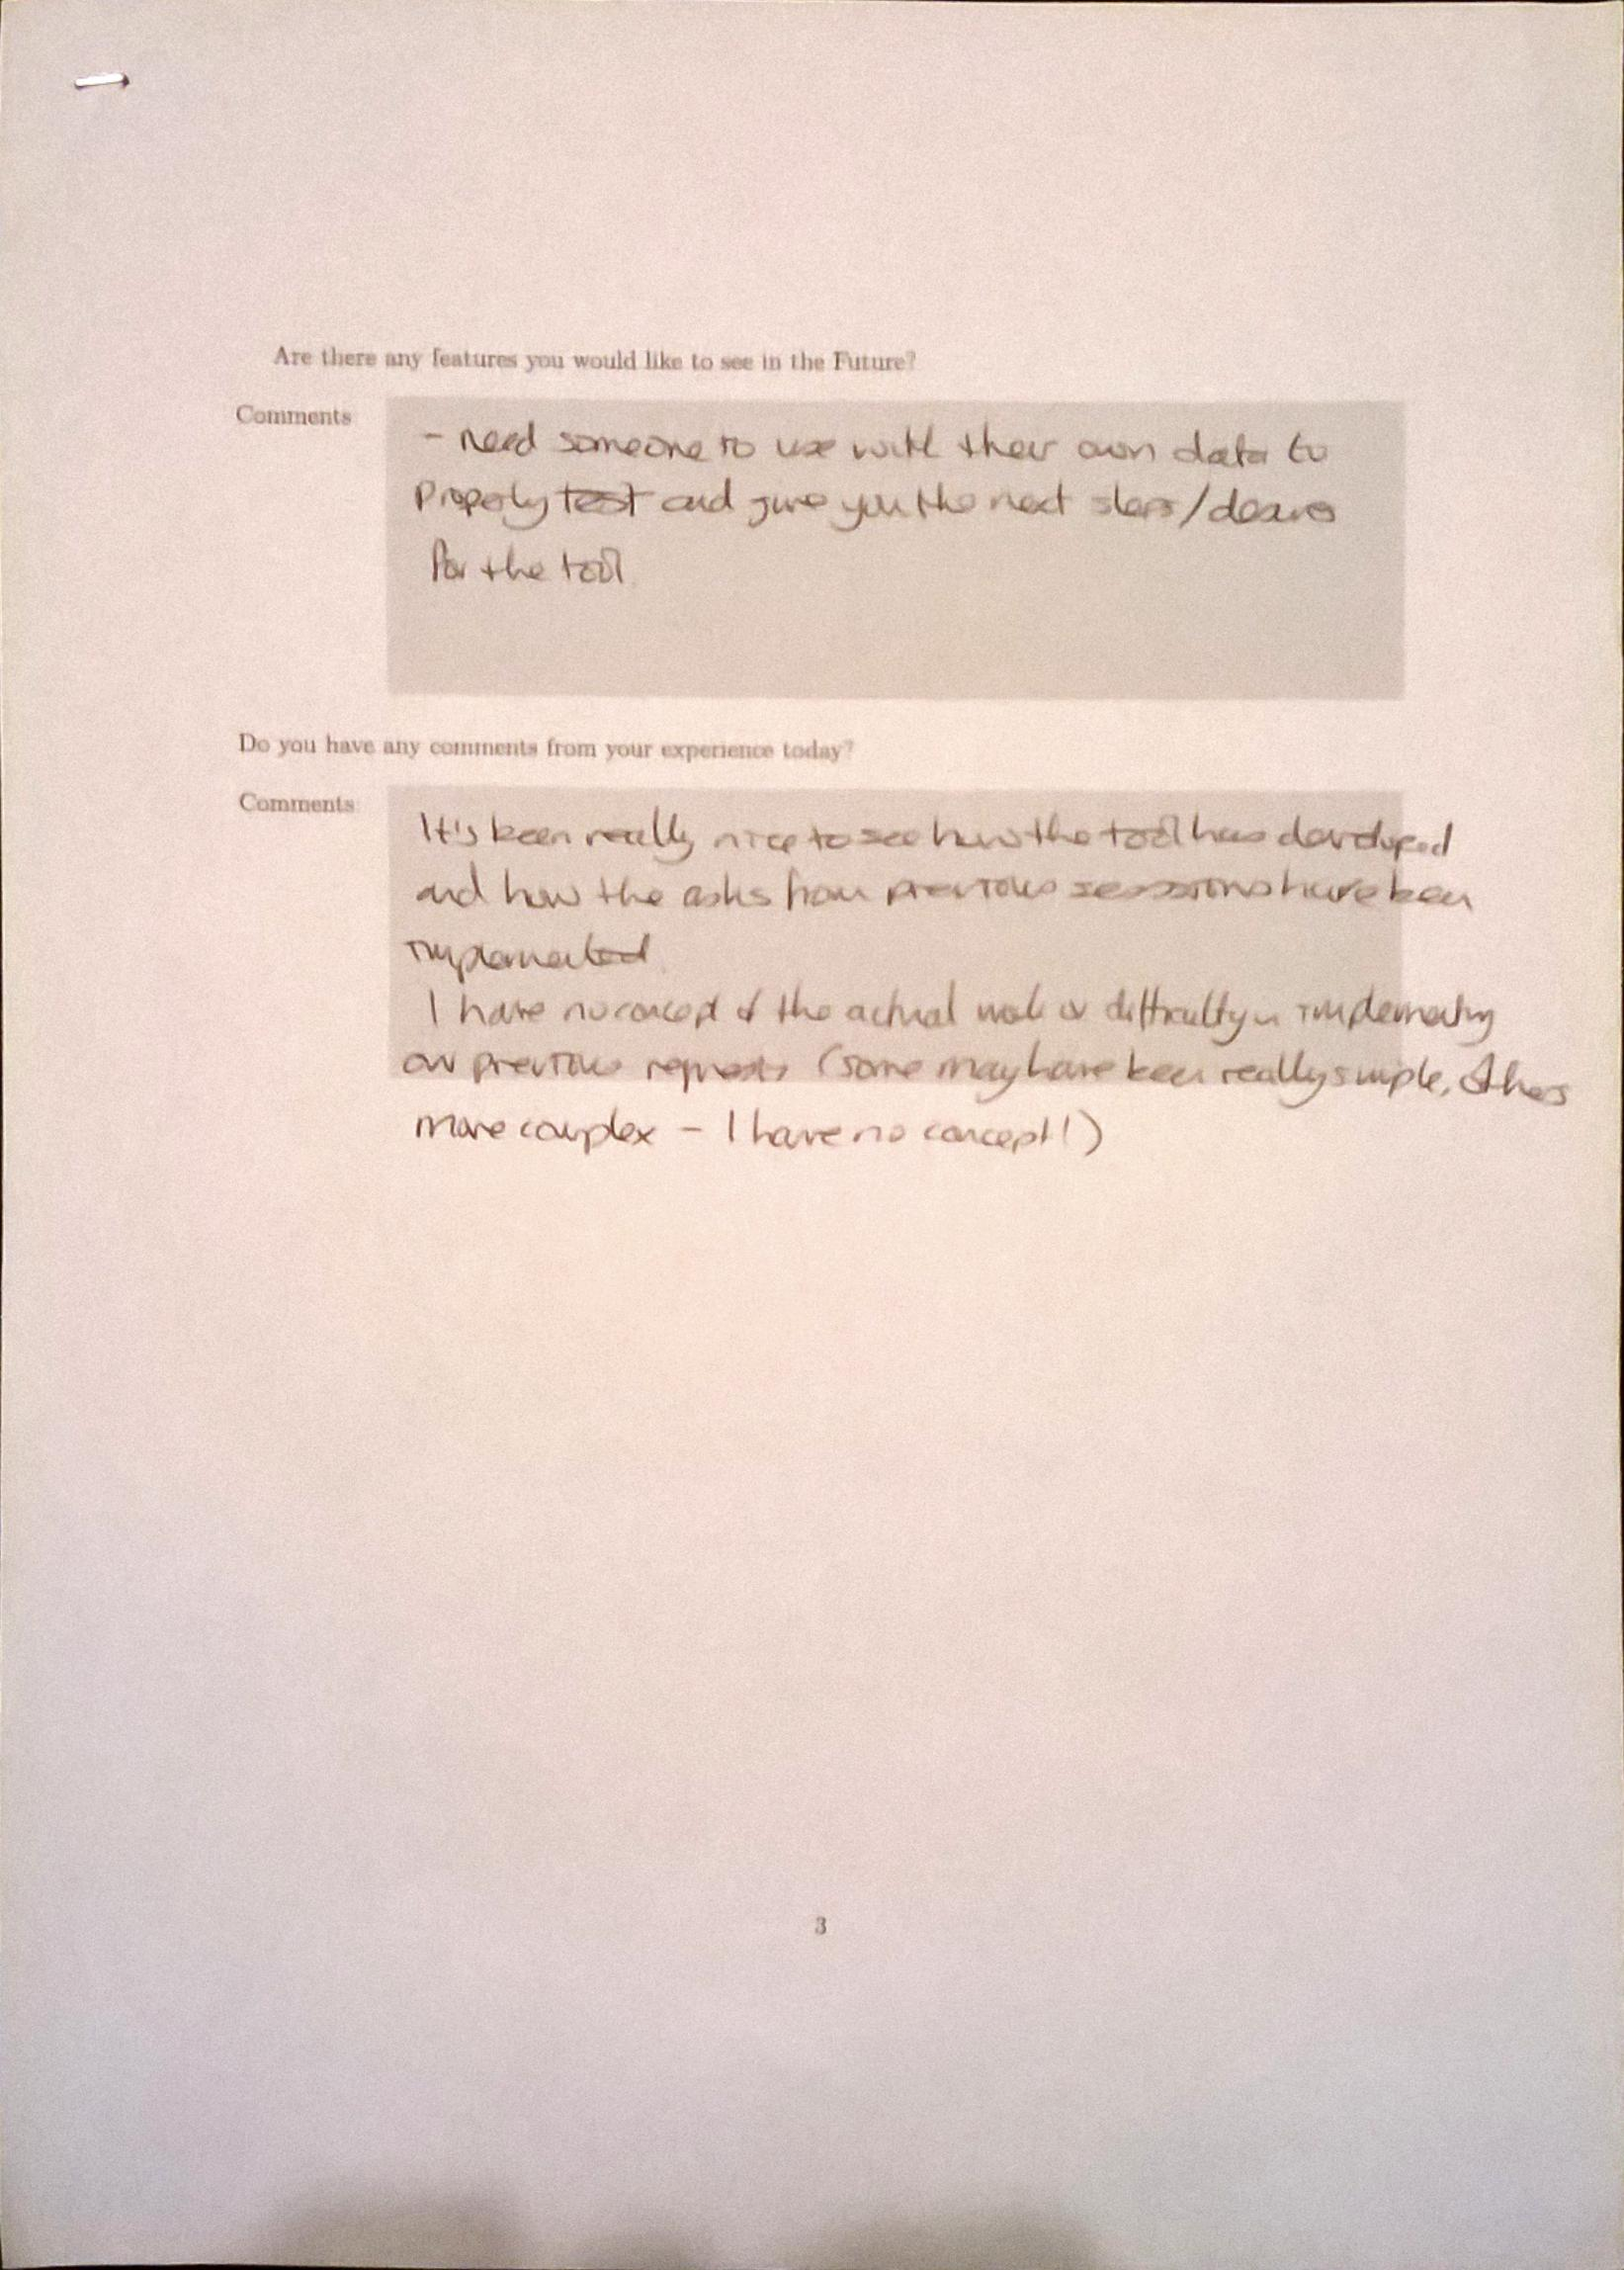
\includegraphics[width=0.95\textwidth]{images/user_eval/user_eval_20.jpg}
    \caption{Third Evaluation}
\end{figure}

\begin{figure}[h!]
    \centering
    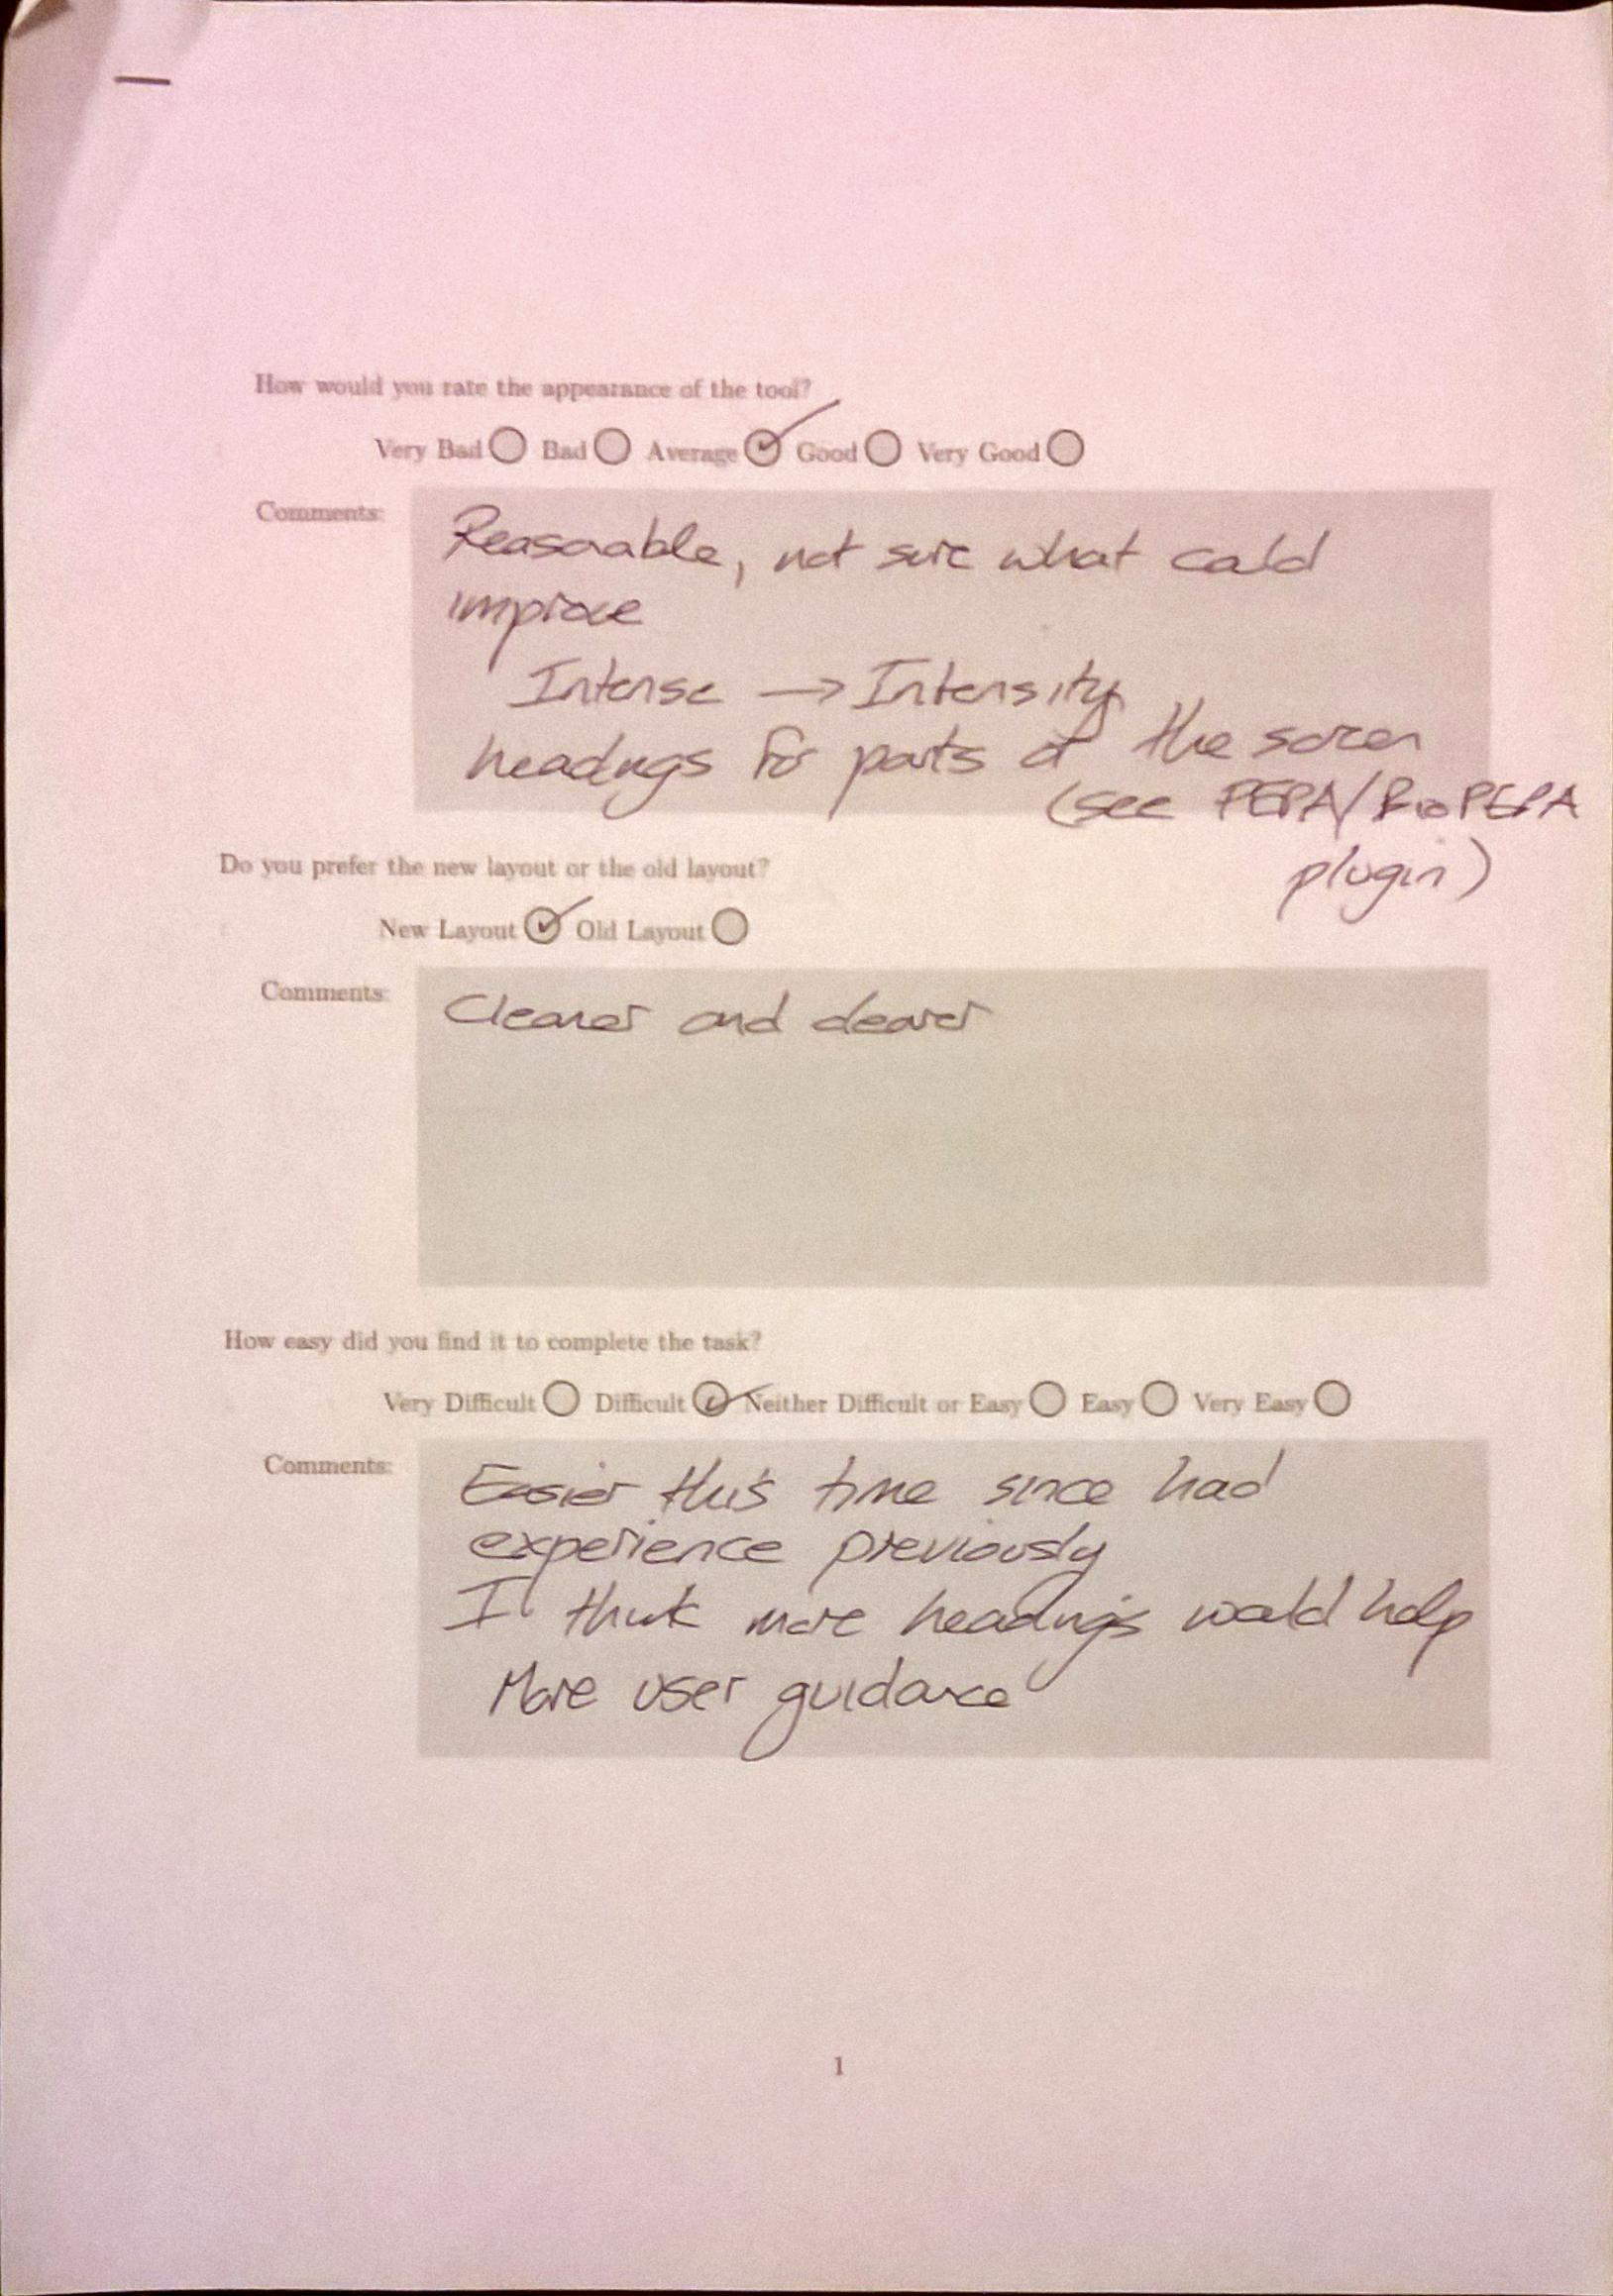
\includegraphics[width=0.95\textwidth]{images/user_eval/user_eval_21.jpg}
    \caption{Third Evaluation}
\end{figure}

\begin{figure}[h!]
    \centering
    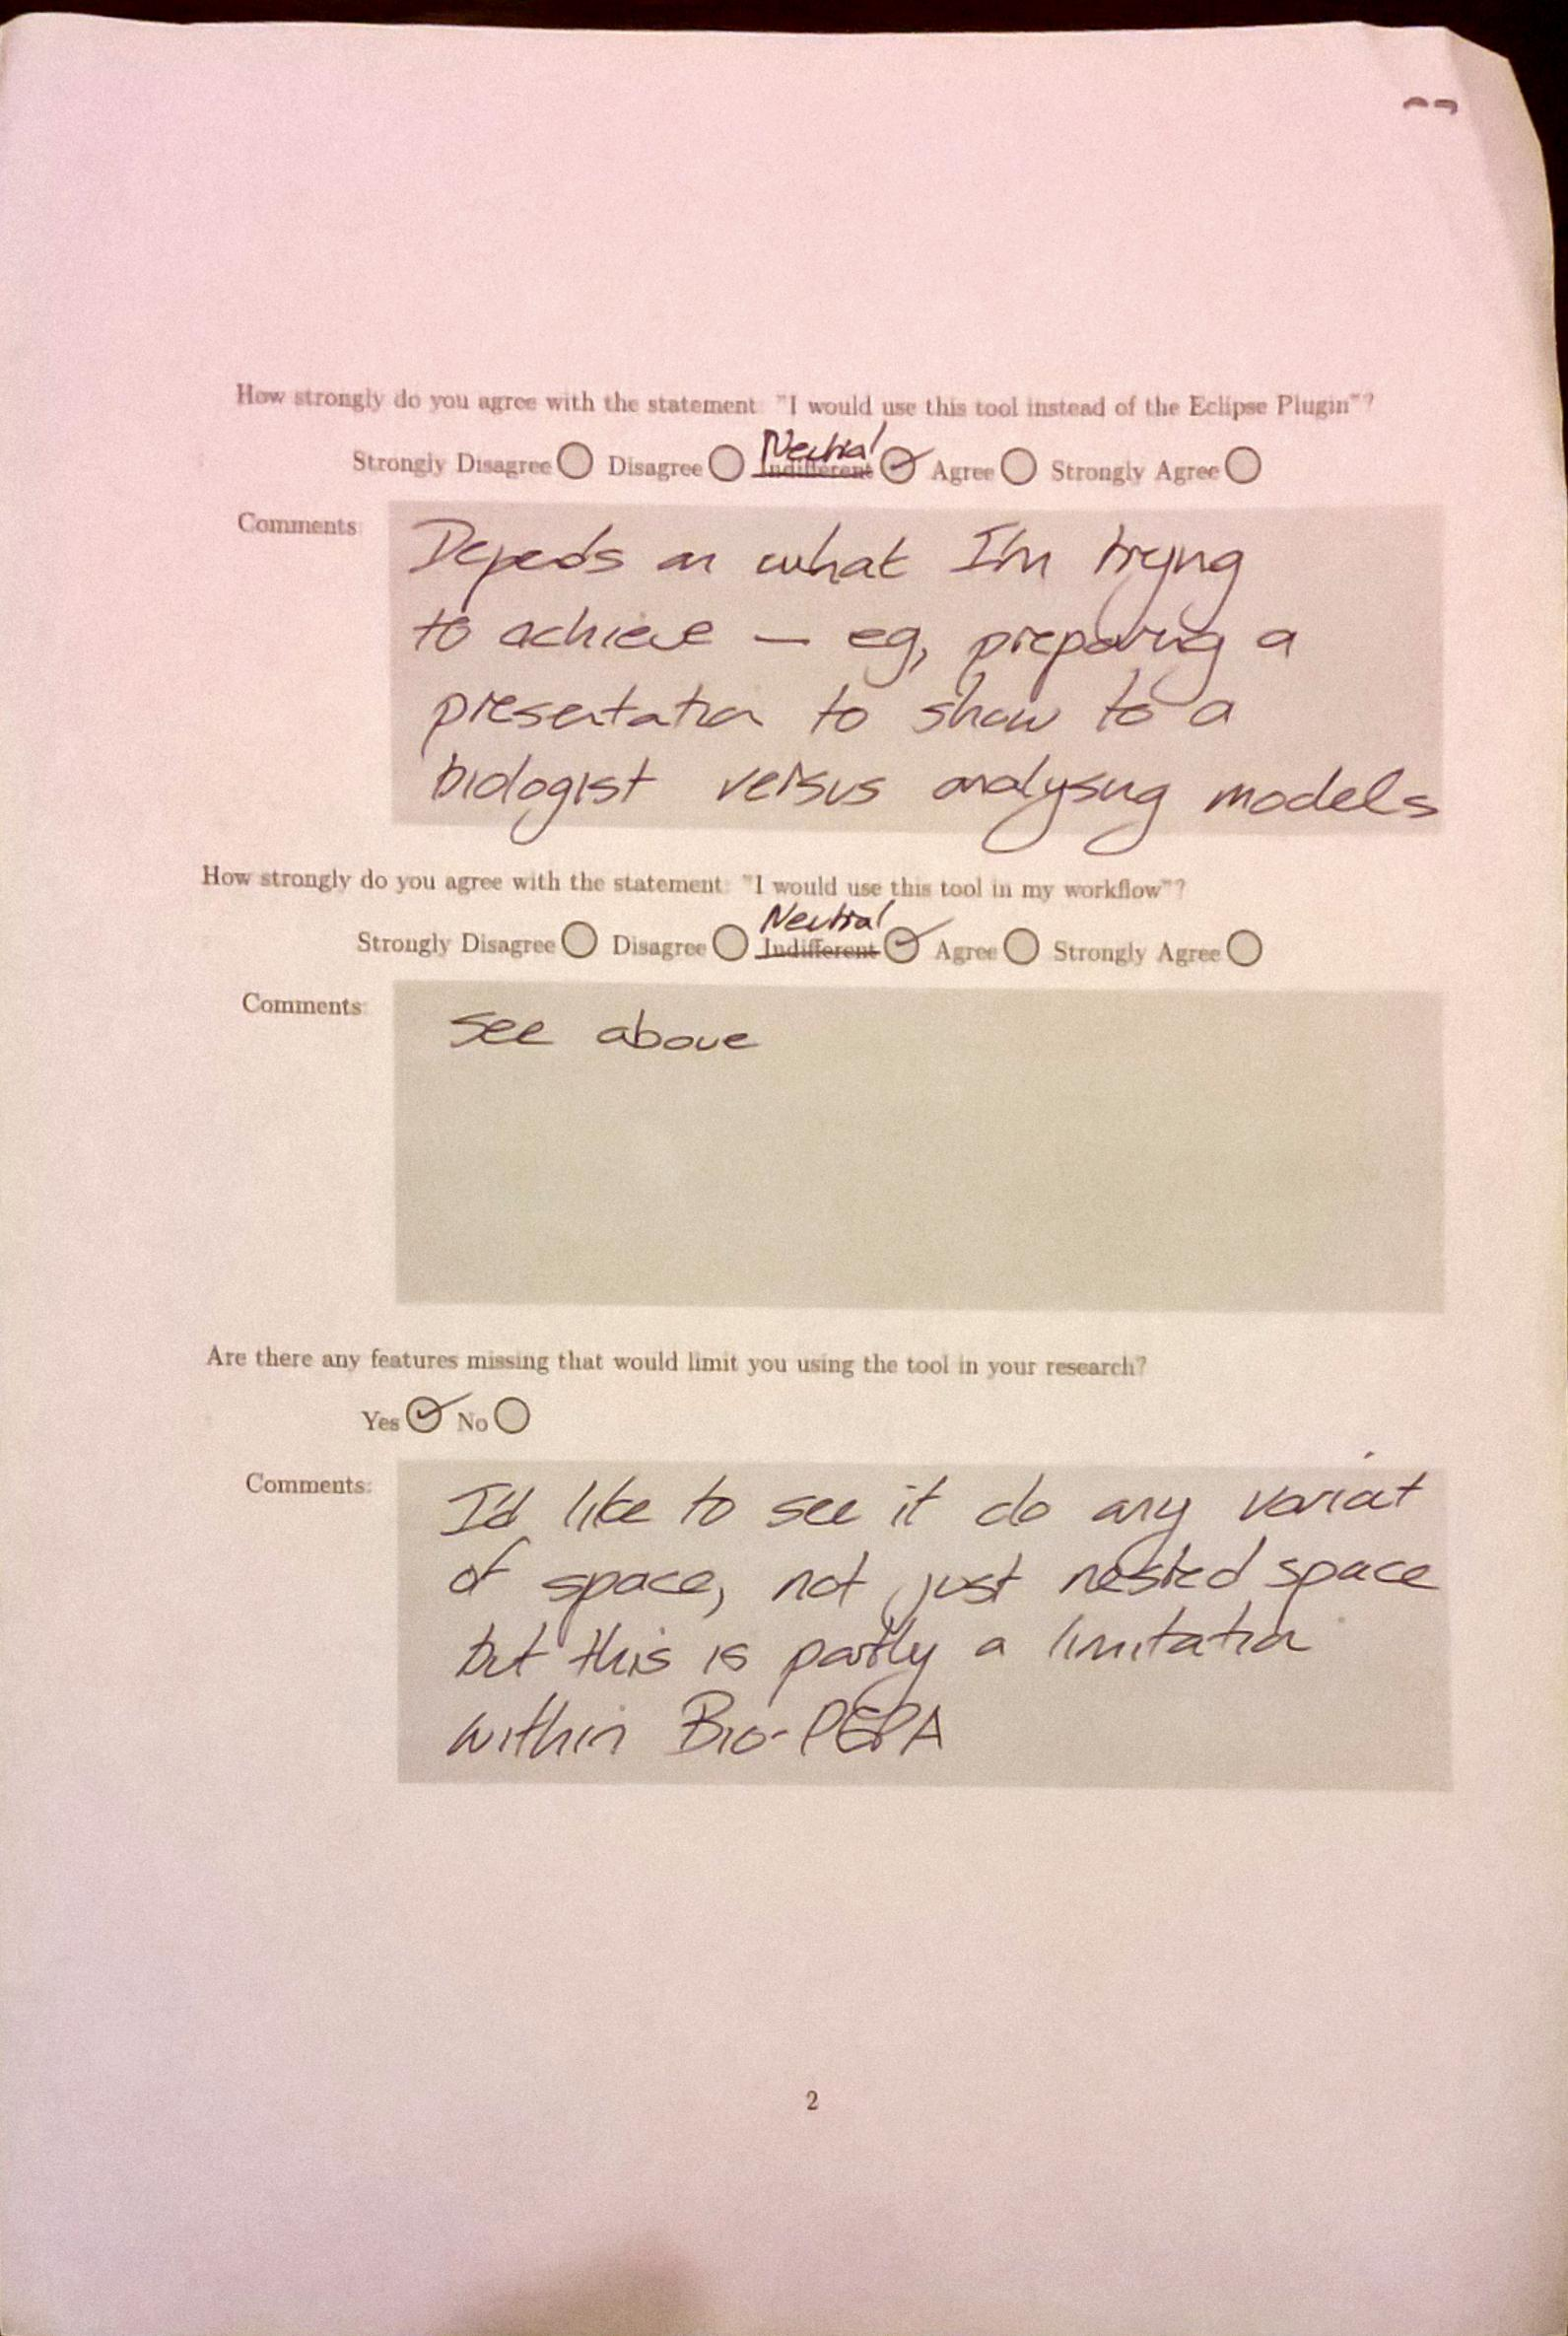
\includegraphics[width=0.95\textwidth]{images/user_eval/user_eval_22.jpg}
    \caption{Third Evaluation}
\end{figure}

\begin{figure}[h!]
    \centering
    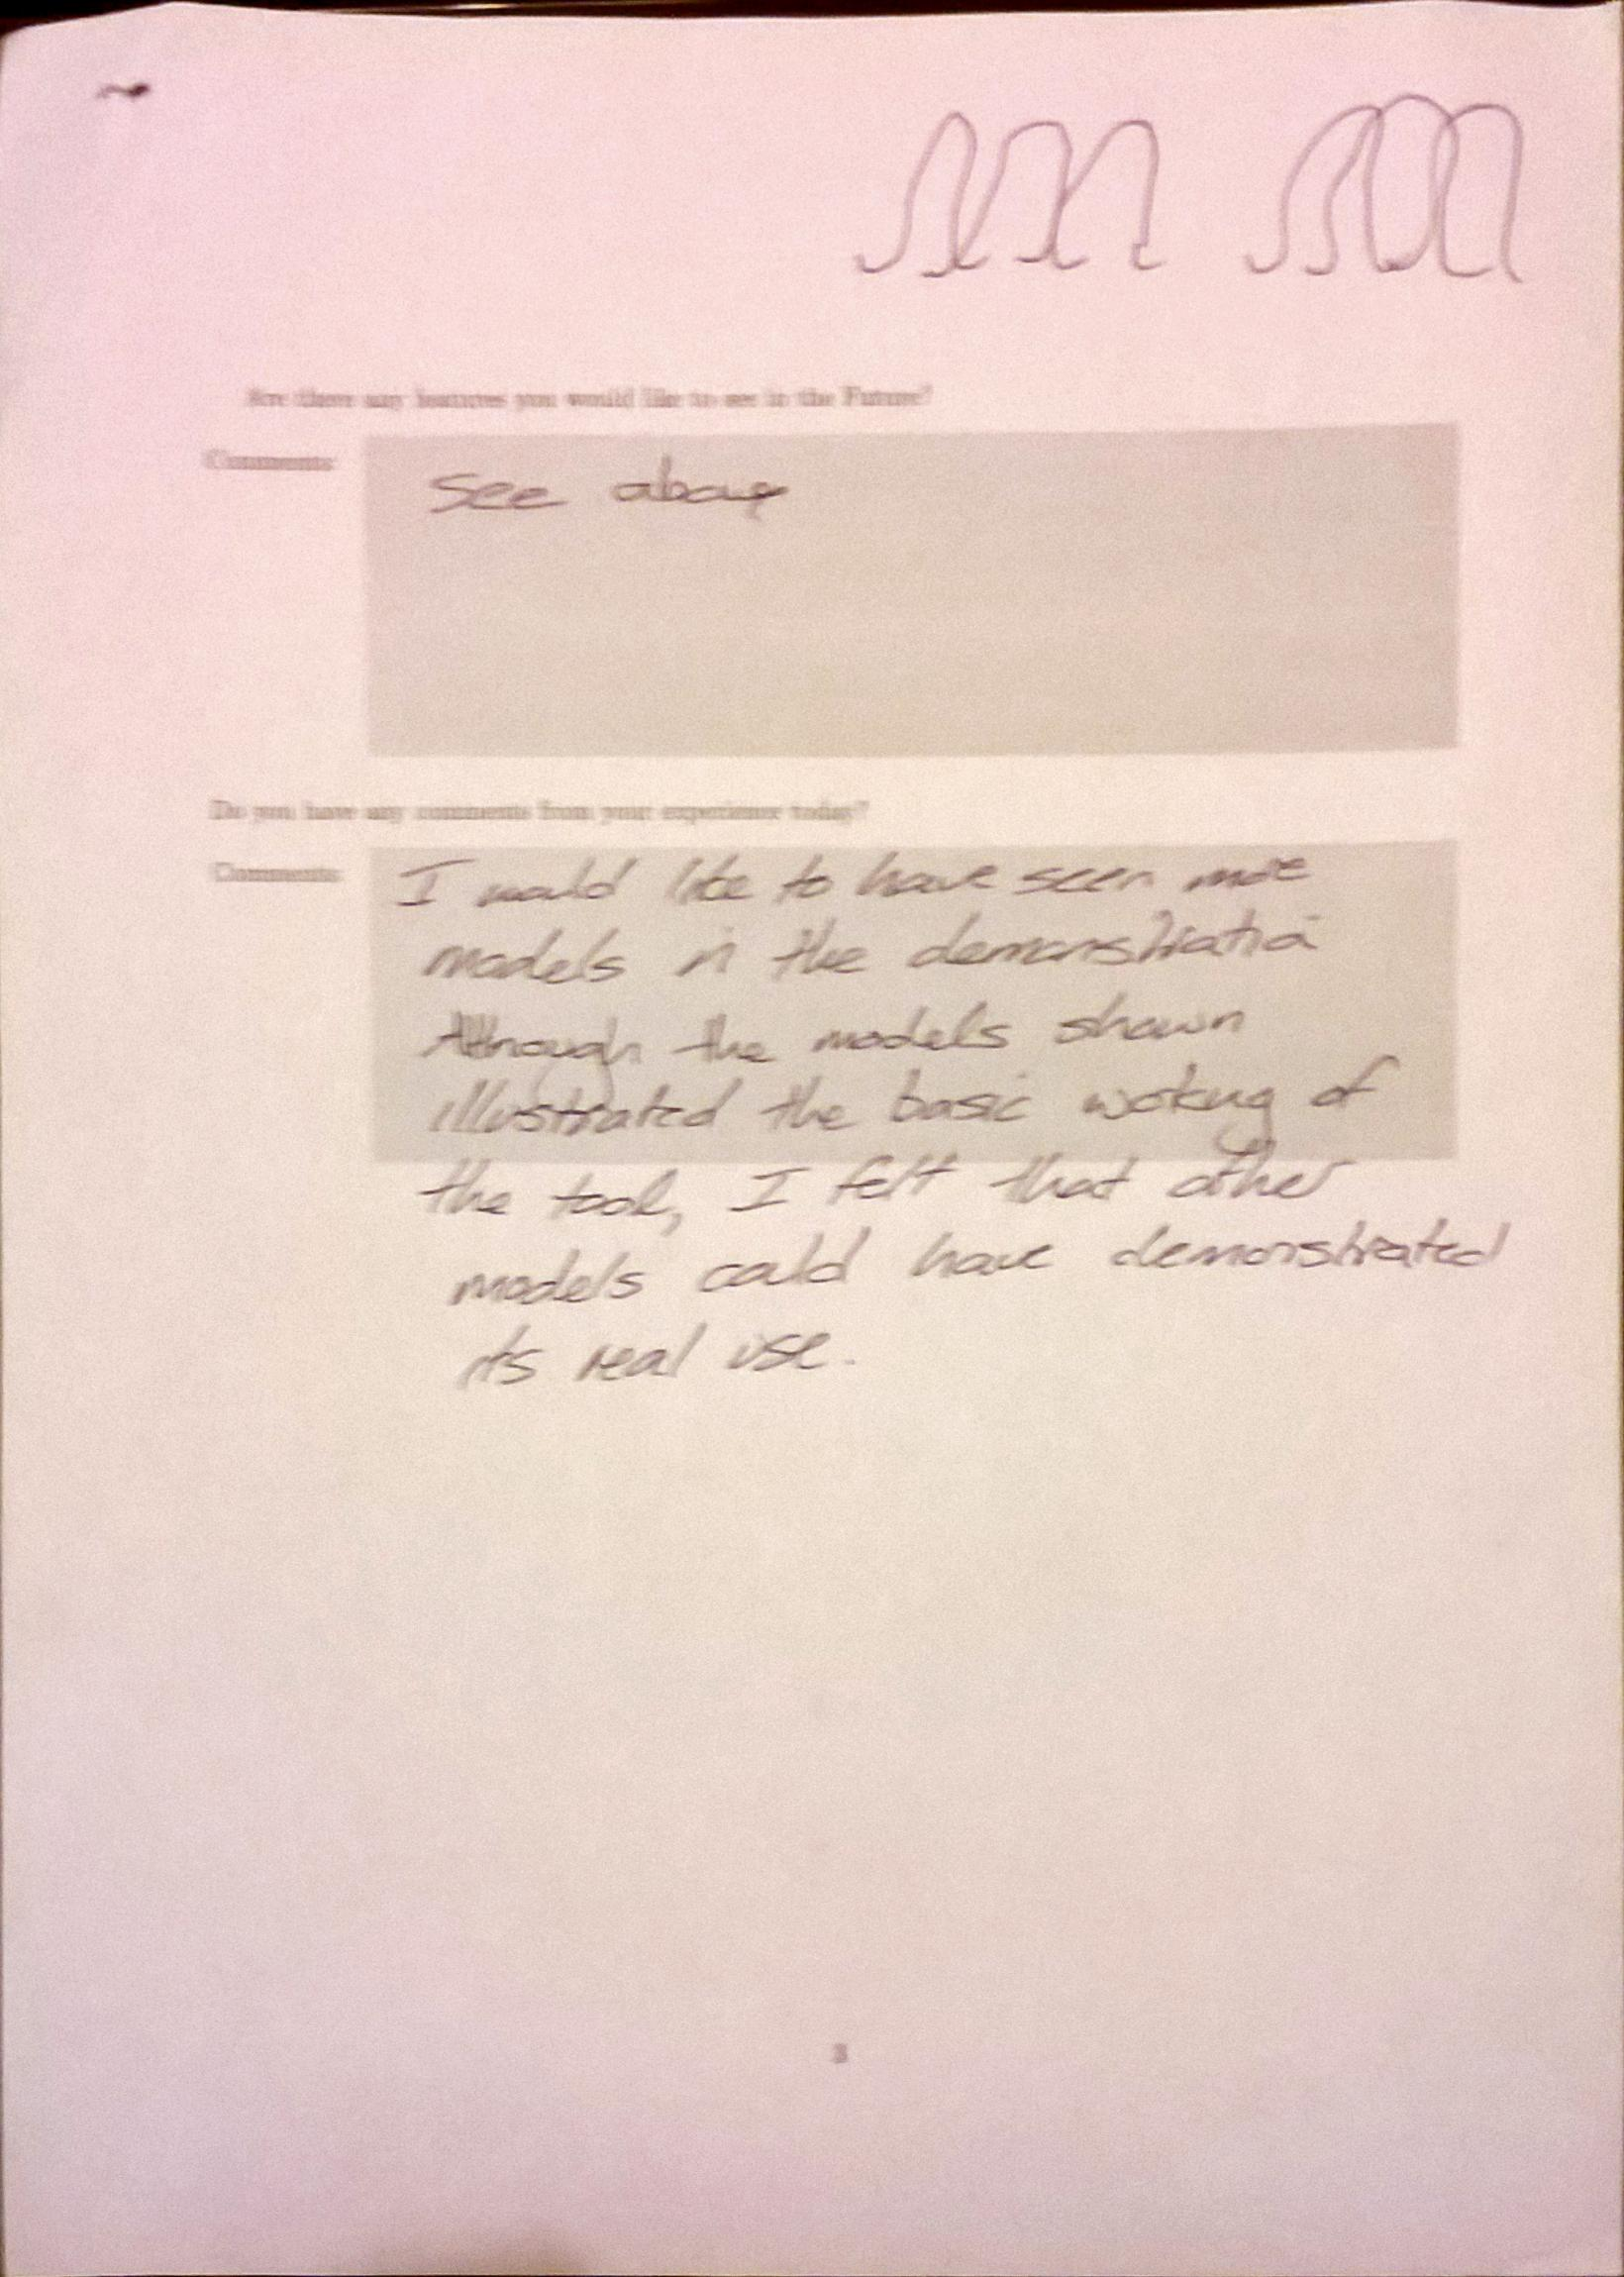
\includegraphics[width=0.95\textwidth]{images/user_eval/user_eval_23.jpg}
    \caption{Third Evaluation}
\end{figure}

\clearpage

\section{Similar Plots}
\label{sec:mutants}

This appendix contains the set of similar plots generated by mutation.  Figure~\ref{fig:query} contains the query plot that the mutations are based on.  The other figures contain the query plot and the mutant.  In the other figures the blue line is the query plot and the green line is the mutation.

\begin{figure}[h!]
    \centering
    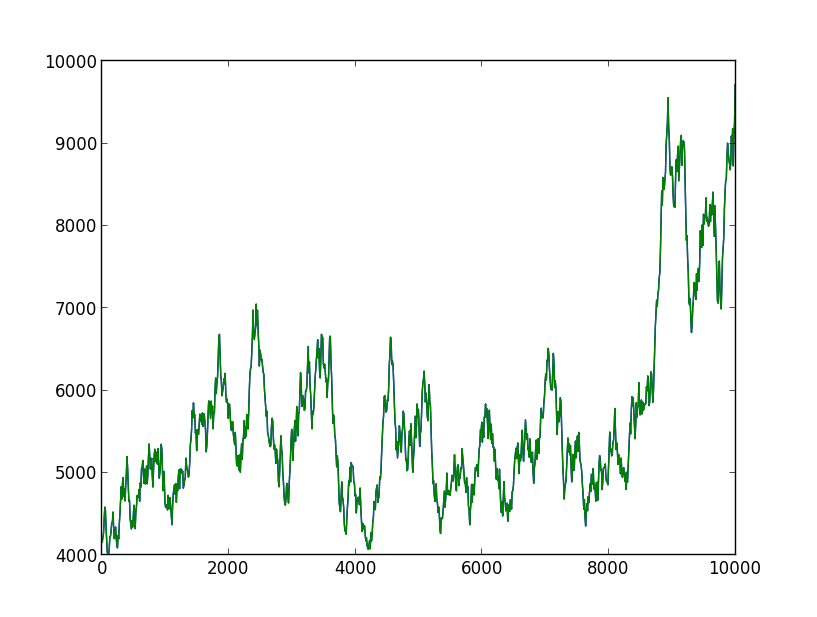
\includegraphics[width=0.7\textwidth]{images/query.png}
    \caption{Query plot}
    \label{fig:query}
\end{figure}

\begin{figure}[h!]
    \centering
    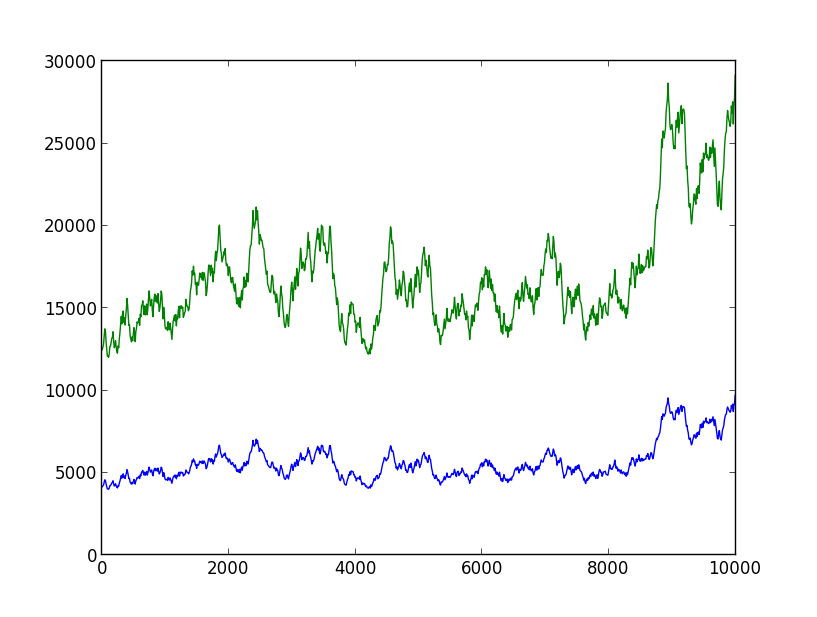
\includegraphics[width=0.7\textwidth]{images/mutant_1.png}
    \caption{First similar plot.  It is a scaling of the original plot by a factor of 3.}
    \label{fig:mutant_1}
\end{figure}

\begin{figure}[h!]
    \centering
    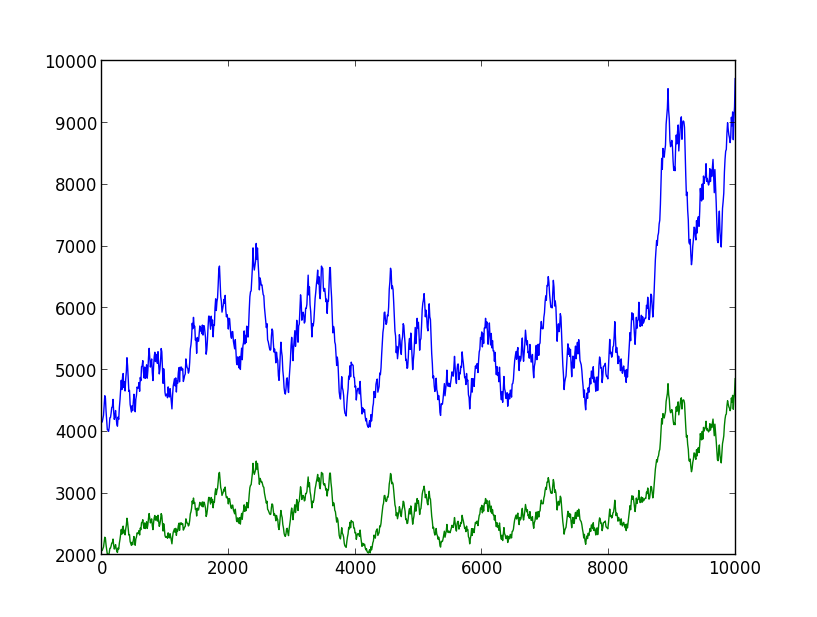
\includegraphics[width=0.7\textwidth]{images/mutant_2.png}
    \caption{Second similar plot.  It is a scaling of the original plot by a factor of 0.5.}
    \label{fig:mutant_2}
\end{figure}

\begin{figure}[h!]
    \centering
    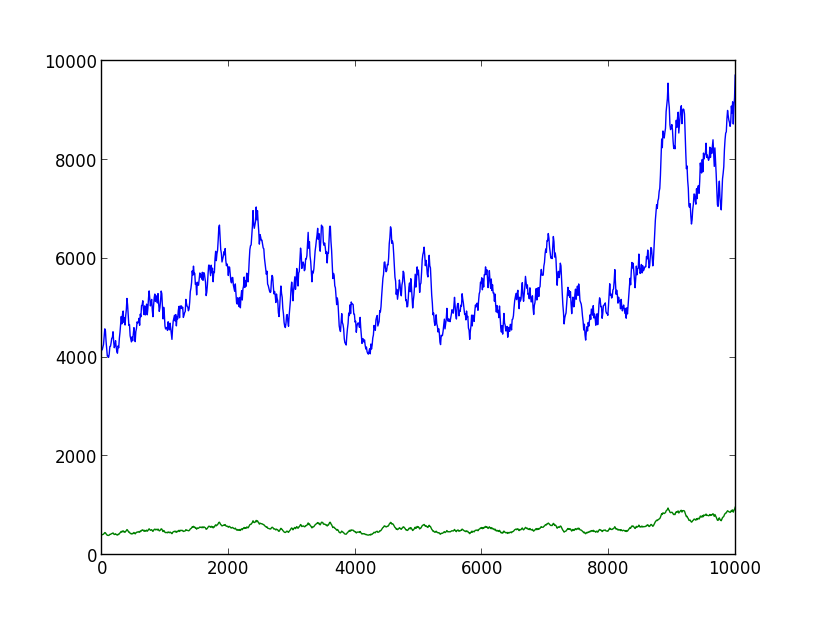
\includegraphics[width=0.7\textwidth]{images/mutant_3.png}
    \caption{Third similar plot.  It is a scaling of the original plot by a factor of 0.1.}
    \label{fig:mutant_3}
\end{figure}

\begin{figure}[h!]
    \centering
    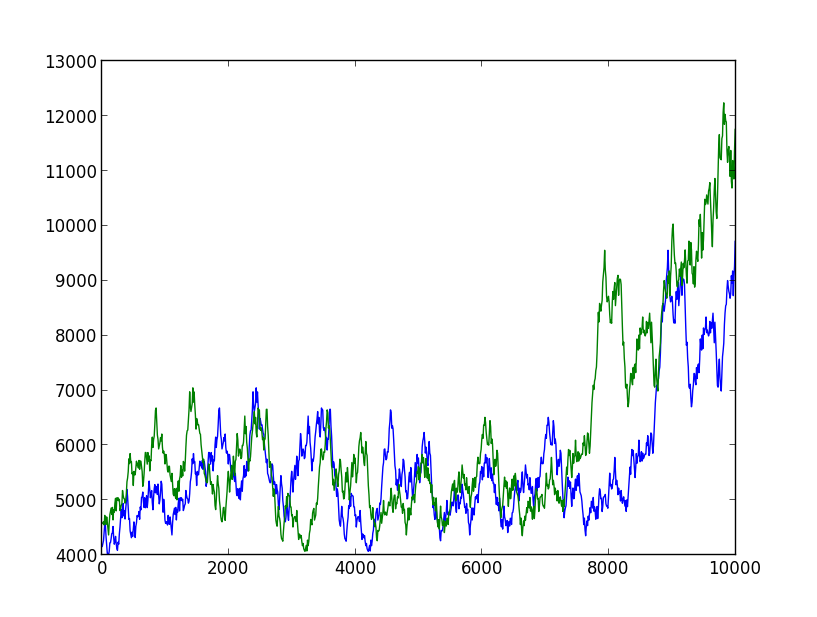
\includegraphics[width=0.7\textwidth]{images/mutant_4.png}
    \caption{Fourth similar plot.  The plot has been shifted left by 10\%.}
    \label{fig:mutant_4}
\end{figure}

\begin{figure}[h!]
    \centering
    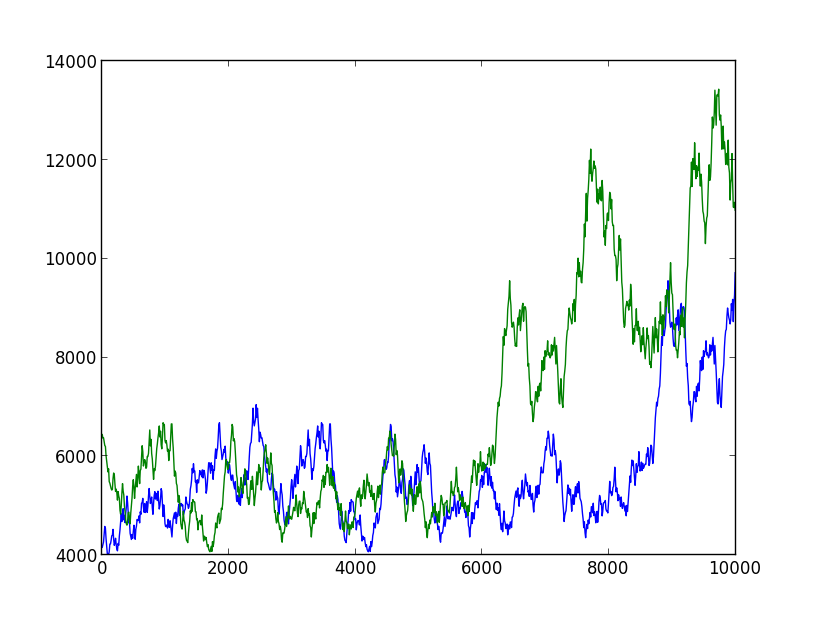
\includegraphics[width=0.7\textwidth]{images/mutant_5.png}
    \caption{Fifth similar plot.  The plot has been shifted left by 25\%.}
    \label{fig:mutant_5}
\end{figure}

\begin{figure}[h!]
    \centering
    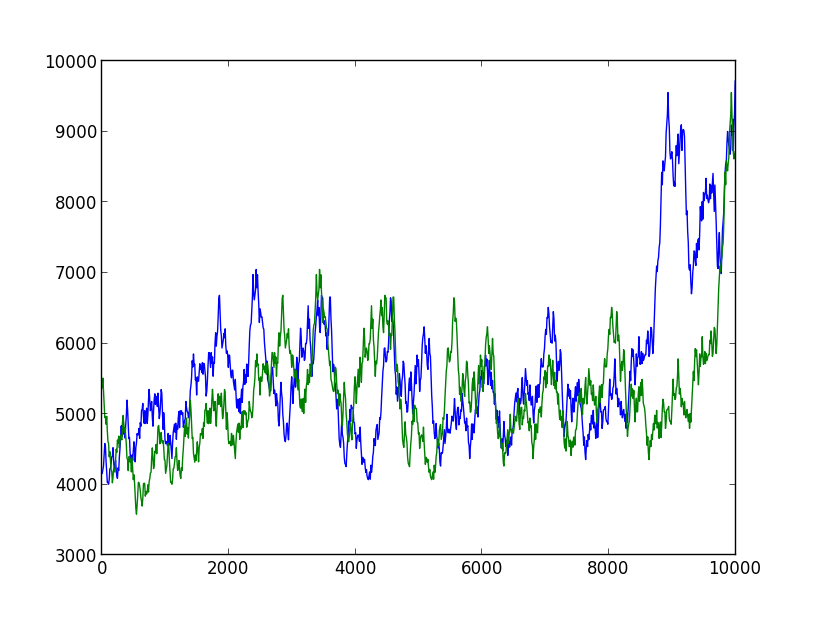
\includegraphics[width=0.7\textwidth]{images/mutant_6.png}
    \caption{Sixth similar plot.  The plot has been shifted right by 10\%.}
    \label{fig:mutant_6}
\end{figure}

\begin{figure}[h!]
    \centering
    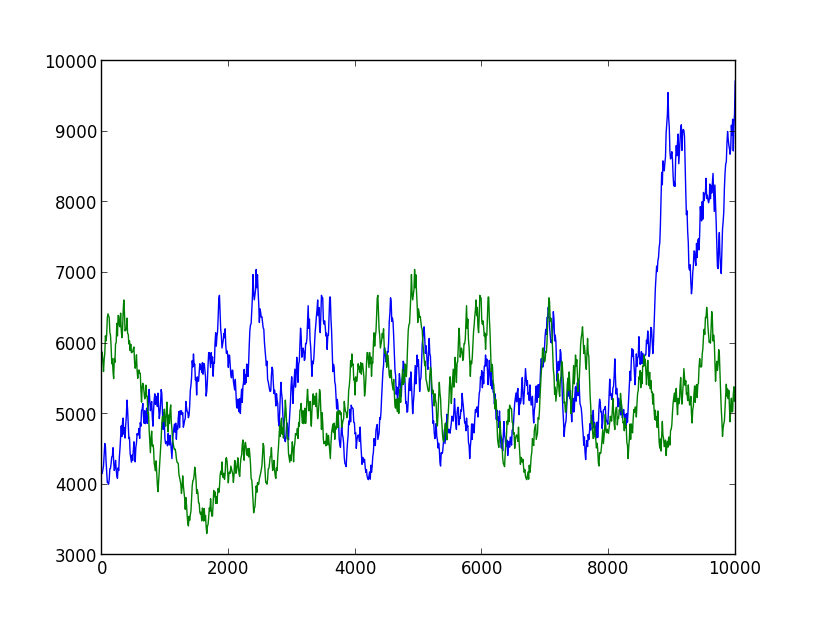
\includegraphics[width=0.7\textwidth]{images/mutant_7.png}
    \caption{Seventh similar plot.  The plot has been shifted right by 25\%.}
    \label{fig:mutant_7}
\end{figure}

\begin{figure}[h!]
    \centering
    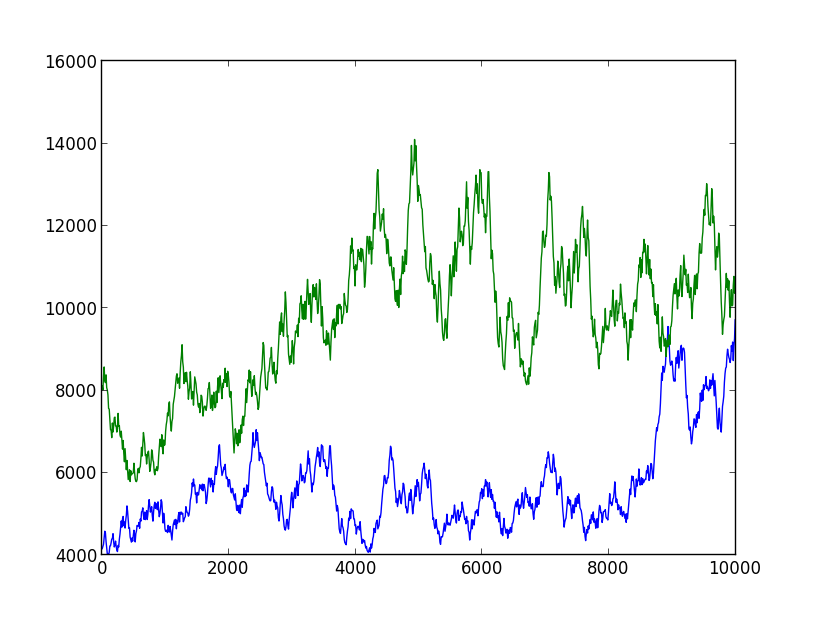
\includegraphics[width=0.7\textwidth]{images/mutant_8.png}
    \caption{Eighth similar plot.  The plot has been shifted right by 25\% and scaled by a factor of 2.}
    \label{fig:mutant_8}
\end{figure}

\begin{figure}[h!]
    \centering
    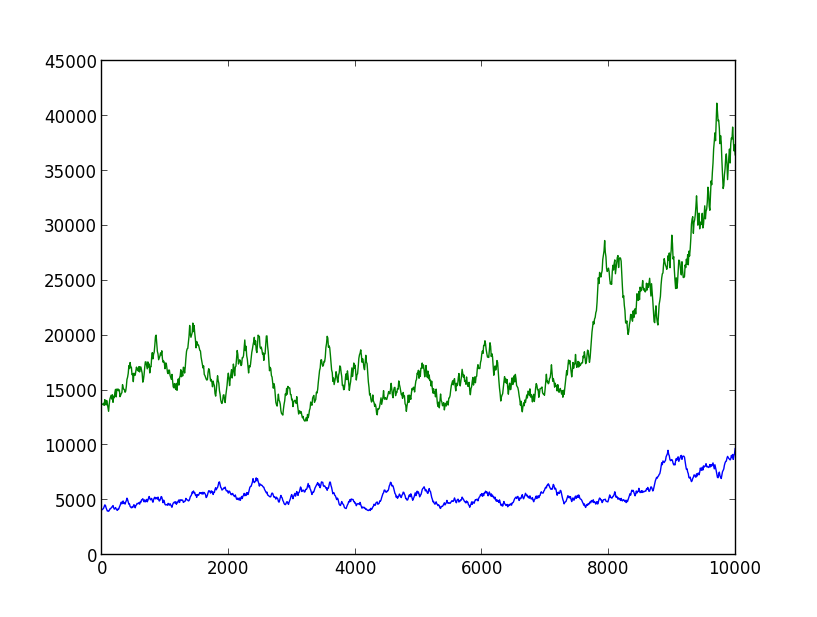
\includegraphics[width=0.7\textwidth]{images/mutant_9.png}
    \caption{Ninth similar plot.  The plot has been shifted left by 10\% and scaled by a factor of 3.}
    \label{fig:mutant_9}
\end{figure}

\begin{figure}[h!]
    \centering
    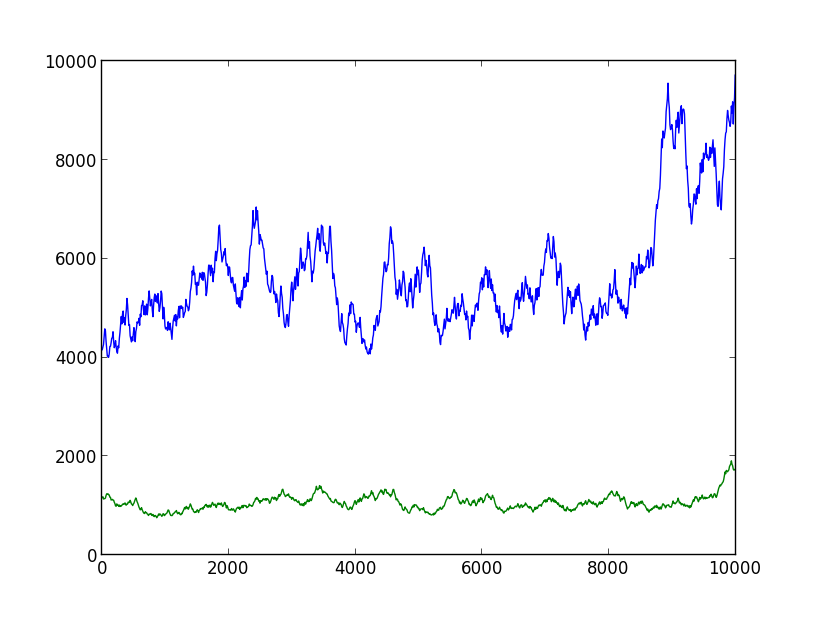
\includegraphics[width=0.7\textwidth]{images/mutant_10.png}
    \caption{Tenth similar plot.  The plot has been shifted right by 10\% and scaled by a factor of 0.2.}
    \label{fig:mutant_10}
\end{figure}

\clearpage

\section{Experiment 1 Graphs}
\label{sec:experiment1}

These are the plots for the results of Experiment 1 in Section~\ref{sec:search_eval}.  In all the graphs the query plot is the blue line and the plot determined to be similar is green.

\begin{figure}[h!]
    \centering
    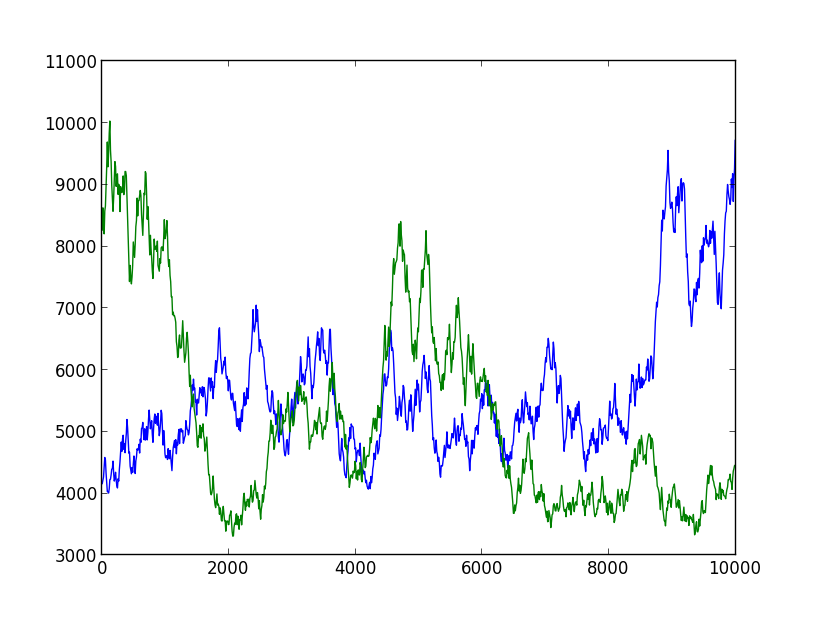
\includegraphics[width=0.7\textwidth]{images/256.png}
    \caption{First similar plot.  Line 256}
    \label{fig:ex1_1}
\end{figure}

\begin{figure}[h!]
    \centering
    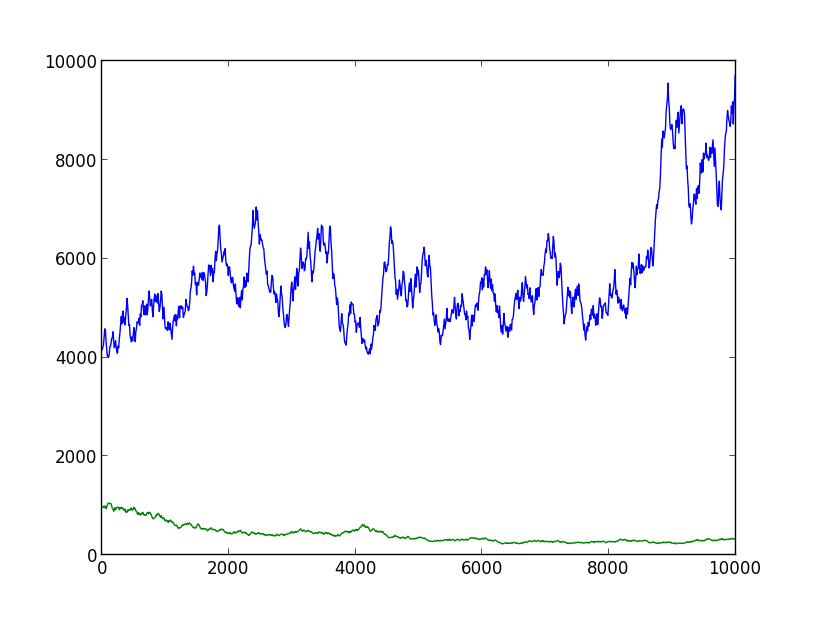
\includegraphics[width=0.7\textwidth]{images/7017.png}
    \caption{Second similar plot.  Line 7017}
    \label{fig:ex1_2}
\end{figure}

\begin{figure}[h!]
    \centering
    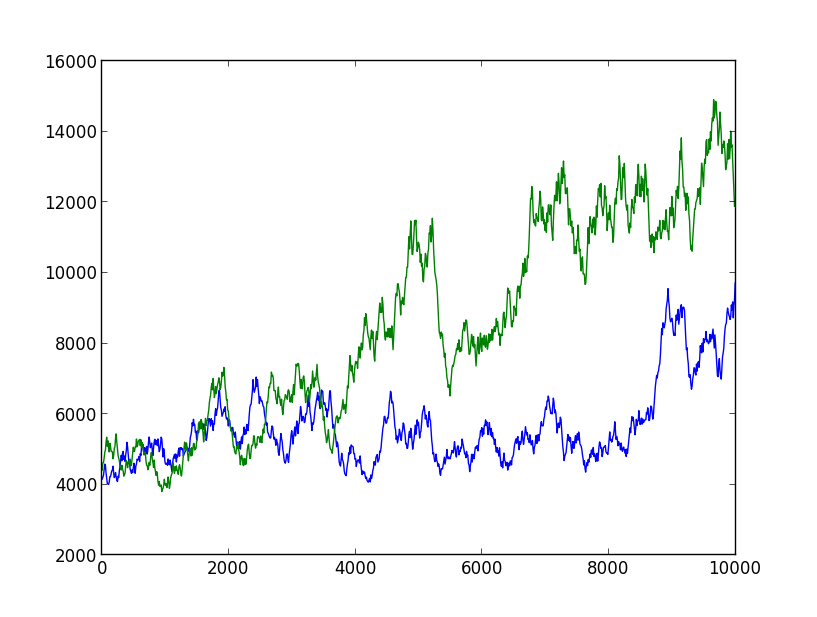
\includegraphics[width=0.7\textwidth]{images/8341.png}
    \caption{Third similar plot.  Line 8341}
    \label{fig:ex1_3}
\end{figure}

\begin{figure}[h!]
    \centering
    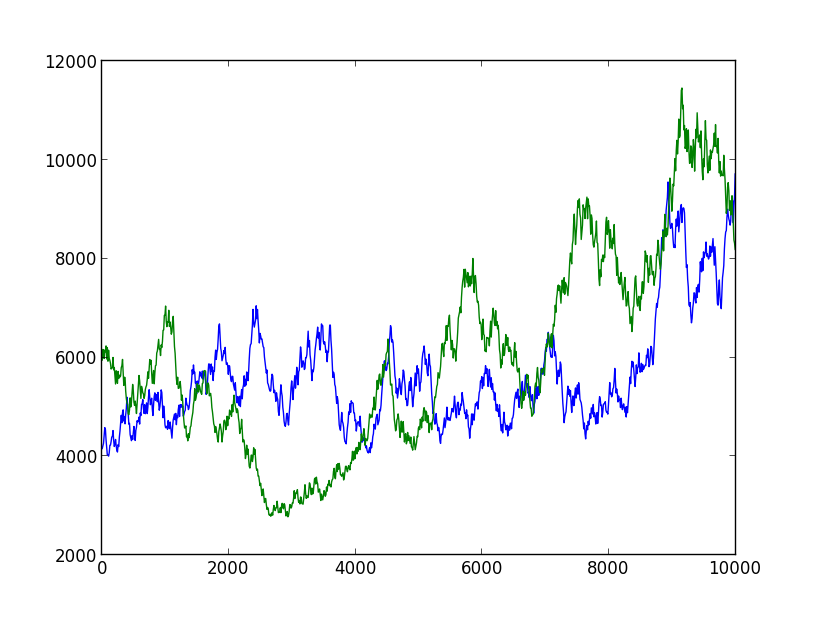
\includegraphics[width=0.7\textwidth]{images/1380.png}
    \caption{Fourth similar plot.  Line 1380}
    \label{fig:ex1_4}
\end{figure}

\begin{figure}[h!]
    \centering
    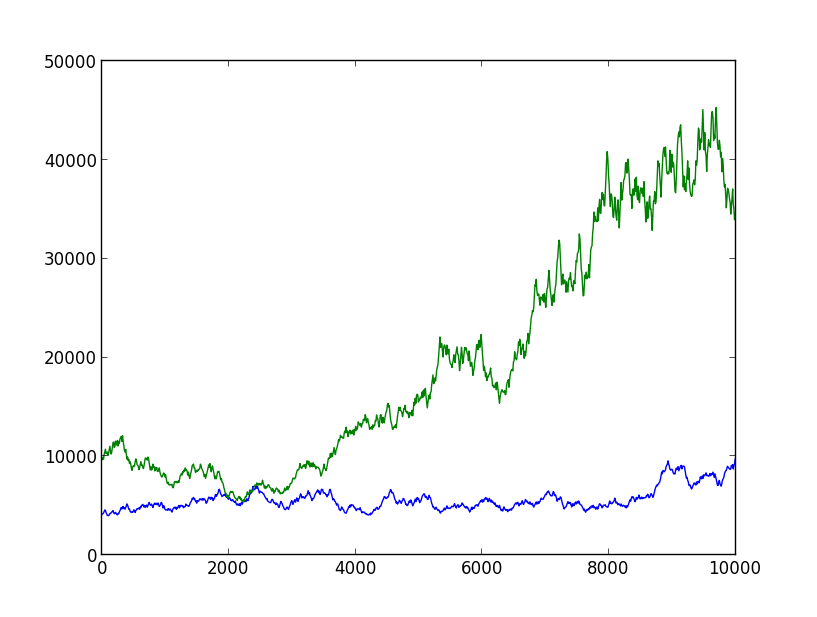
\includegraphics[width=0.7\textwidth]{images/4997.png}
    \caption{Fifth similar plot.  Line 4997}
    \label{fig:ex1_5}
\end{figure}

\begin{figure}[h!]
    \centering
    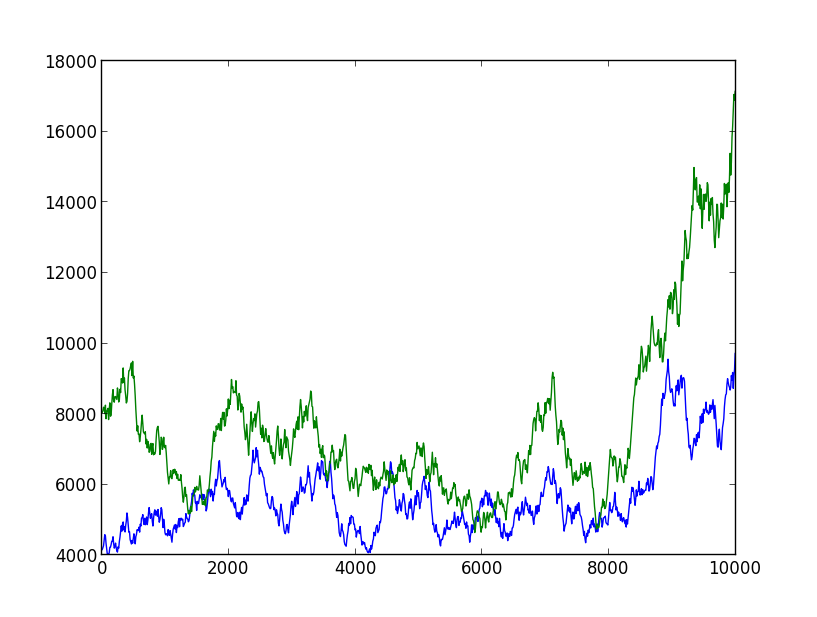
\includegraphics[width=0.7\textwidth]{images/5462.png}
    \caption{Sixth similar plot.  Line 5462}
    \label{fig:ex1_6}
\end{figure}

\begin{figure}[h!]
    \centering
    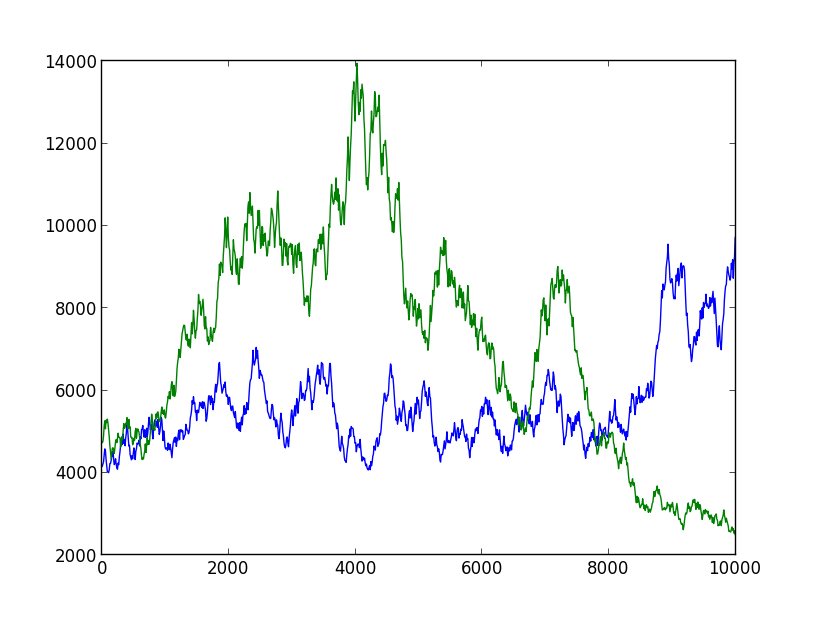
\includegraphics[width=0.7\textwidth]{images/6648.png}
    \caption{Seventh similar plot.  Line 6648}
    \label{fig:ex1_7}
\end{figure}

\begin{figure}[h!]
    \centering
    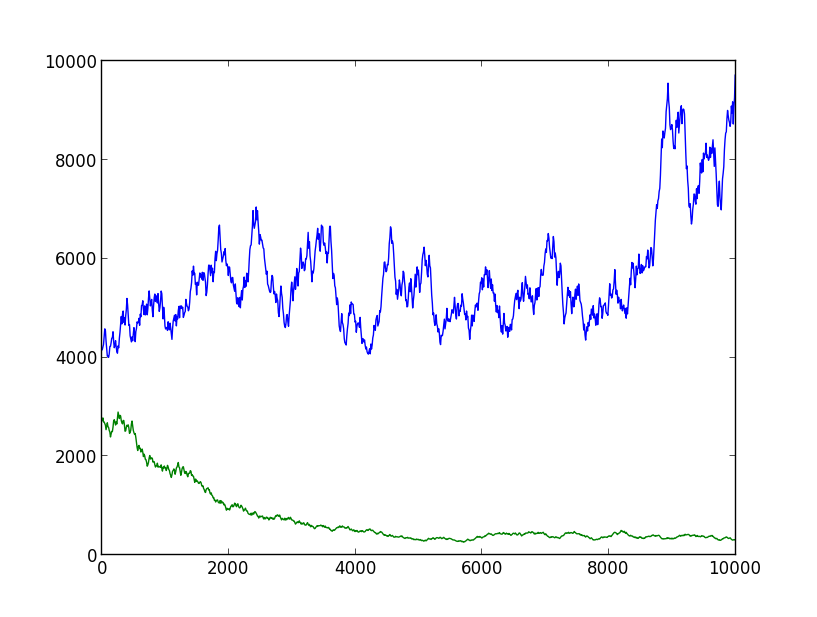
\includegraphics[width=0.7\textwidth]{images/2298.png}
    \caption{Eighth similar plot.  Line 2298}
    \label{fig:ex1_8}
\end{figure}

\begin{figure}[h!]
    \centering
    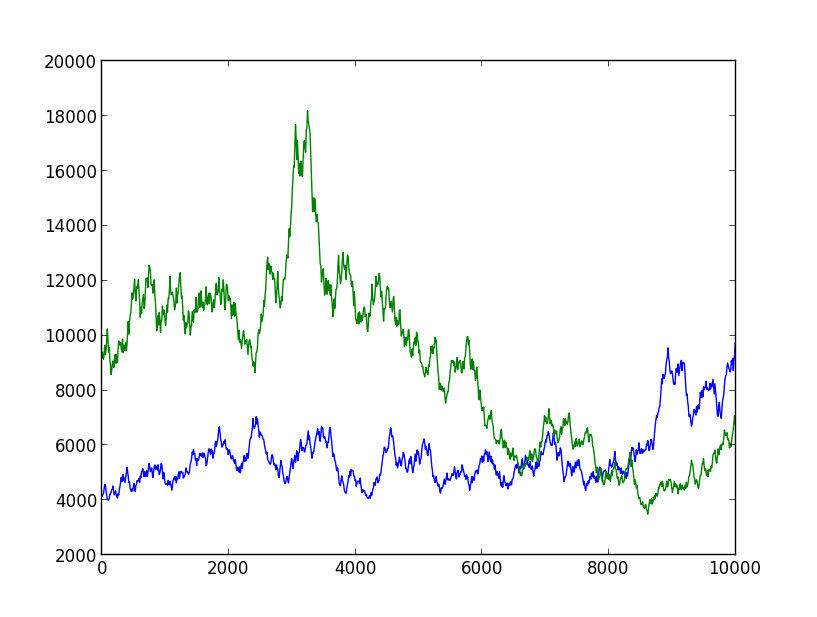
\includegraphics[width=0.7\textwidth]{images/595.png}
    \caption{Ninth similar plot.  Line 595}
    \label{fig:ex1_9}
\end{figure}

\begin{figure}[h!]
    \centering
    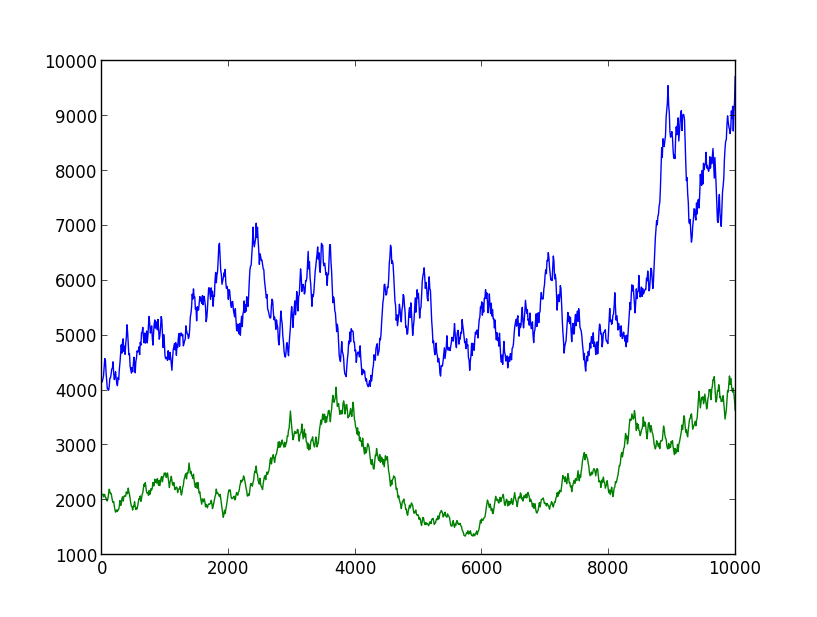
\includegraphics[width=0.7\textwidth]{images/190.png}
    \caption{Tenth similar plot.  Line 190}
    \label{fig:ex1_10}
\end{figure}
